\chapter[A designer FG-Nup that reconstitutes the selective transport barrier of the nuclear pore complex]{A designer FG-Nup that reconstitutes the selective transport barrier of the nuclear pore complex}
\chaptermark{A designer FG-Nup that reconstitutes the selectivity of the NPC}
\label{chapter_4}

%% The following annotation is customary for chapter which have already been
%% published as a paper.
\blfootnote{This chapter has been published as: Alessio Fragasso, Hendrik W. de Vries, John Andersson, Eli O. van der Sluis, Erik van der Giessen, Andreas Dahlin, Patrick R. Onck, Cees Dekker. \emph{A designer FG-Nup that reconstitutes the selective transport barrier of the Nuclear Pore Complex}. Nature Communications 12, 2010 (2021) \cite{Fragasso2021}.}

%% It is only necessary to list the authors if multiple people contributed
%% significantly to the chapter.
%\authors{Albert {\titleshape Einstein}}
%
%%% The '0pt' option ensures that no extra vertical space follows this epigraph,
%%% since there is another epigraph after it.
%\epigraph[0pt]{
%    Nature and nature's laws lay hid in the night; \\
%    God said `Let Newton be!' and all was light.
%}{Alexander Pope}
%
%\epigraph{
%    It did not last: the devil shouting `Ho. \\
%    Let Einstein be!' restore the status quo.
%}{Sir John Collings Squire}

\begin{abstract}
Nuclear Pore Complexes (NPCs) regulate bidirectional transport between the nucleus and the cytoplasm. Intrinsically disordered FG-Nups line the NPC lumen and form a selective barrier, where transport of most proteins is inhibited whereas specific transporter proteins freely pass. The mechanism underlying selective transport through the NPC is still debated. Here, we reconstitute the selective behaviour of the NPC bottom-up by introducing a rationally designed artificial FG-Nup that mimics natural Nups. Using QCM-D, we measure selective binding of the artificial FG-Nup brushes to the transport receptor Kap95 over cytosolic proteins such as BSA. Solid-state nanopores with the artificial FG-Nups lining their inner walls support fast translocation of Kap95 while blocking BSA, thus demonstrating selectivity. Coarse-grained molecular dynamics simulations highlight the formation of a selective meshwork with densities comparable to native NPCs. Our findings show that simple design rules can recapitulate the selective behaviour of native FG-Nups and demonstrate that no specific spacer sequence nor a spatial segregation of different FG-motif types are needed to create selective NPCs. 
\end{abstract}

%% Start the actual chapter on a new page.
\newpage


\section{Introduction}
Nucleocytoplasmic transport is orchestrated by the Nuclear Pore Complex (NPC), which imparts a selective barrier to biomolecules \cite{Wente2000,Wente2010}. The NPC is a large eightfold-symmetric protein complex (with a size of $\sim$52 MDa in yeast and $\sim$112 MDa in vertebrates) that is embedded within the nuclear envelope and comprises $\sim$30 different types of Nucleoporins (Nups) \cite{Kim2018,Reichelt1990}.  Intrinsically disordered proteins, termed FG-Nups, line the central channel of the NPC. FG-Nups are characterized by the presence of phenylalanine-glycine (FG) repeats separated by spacer sequences \cite{Yamada2010} and they are highly conserved throughout species \cite{Terry2009}. FG-Nups carry out a dual function: By forming a dense barrier (100-200 mg/mL) within the NPC lumen, they allow passage of molecules in a selective manner \cite{Bayliss1999,Ghavami2016,Popken2015,Timney2016}. Small molecules can freely diffuse through, whereas larger particles are generally excluded \cite{Lim2006}. At the same time, FG-Nups mediate the transport of large NTR-bound (Nuclear Transport Receptor) cargoes across the NPC through transient hydrophobic interactions between FG repeats and hydrophobic pockets on the convex side of NTRs \cite{Bayliss2000}. Various models have been developed in order to connect the physical properties of FG-Nups to the selective properties of the NPC central channel, e.g. the ‘virtual-gate’ \cite{Rout2003}, ‘selective phase’\cite{Frey2006,Frey2007}, ‘reduction of dimensionality’\cite{Peters2005}, ‘kap-centric’\cite{Kapinos2014,Kapinos2017,Schleicher2014}, ‘polymer brush’\cite{Lim2007}, and ‘forest’\cite{Yamada2010} models.  No consensus on the NPC transport mechanisms has yet been reached. 


The NPC is highly complex in its architecture and dynamics, being constituted by many different Nups that simultaneously interact with multiple transiting cargoes and NTRs. In fact, the NTRs with their cargoes may amount to almost half of the mass of the central channel, so they may be considered an intrinsic part of the NPC3. These NPC properties complicate in-vivo studies \cite{Kim2018,Adams2016,Yang2004,Ma2016}, for which it is very challenging to identify contributions coming from individual FG-Nups \cite{Beck2016,Lin2019}. On the other hand, in-vitro approaches to study nucleocytoplasmic transport using biomimetic NPC systems \cite{Jovanovic-Talisman2009,Eisele2010a,Kowalczyk2011a,Kapinos2014,Schmidt2015,Ananth2018,Fisher2018,Ketterer2018} have thus far been limited to single native FG-Nups and mutations thereof, attempting to understand the physical behaviour of FG-Nups and their interactions with NTRs. The reliance on a few selected Nups from yeast or humans in these studies with sequences that evolved over time in different ways for each of these specific organisms makes it difficult to pinpoint the essential and minimal properties that provide FG-Nups with their specific selective functionality. 


Here, we describe a bottom-up approach to studying nuclear transport selectivity, where we rationally design, synthesize, and assess artificial FG-Nups with user-defined properties that are set by an amino acid sequence that is chosen by the user. With this approach we address the question: can we build a synthetic protein that mimics the selective behaviour of native FG-Nups? By combining experiments and coarse-grained molecular dynamics simulations, we illustrate the design and synthesis of an artificial 311-residue long FG-Nup, which we coin NupX, and characterize its selective behaviour with respect to Kap95 (a well-characterized NTR from yeast, 95 kDa) versus Bovine Serum Albumin (BSA, 66 kDa). Firstly, we explore the interactions between Kap95 and NupX brushes with varying grafting densities using quartz crystal microbalance with dissipation monitoring (QCM-D), finding that NupX brushes bind Kap95 while showing no binding to BSA. We confirm this finding by calculating the potential of mean force (PMF) associated with the entry of Kap95 or an inert cargo into NupX brushes. Secondly, we explore the transport properties of NupX-functionalized solid-state nanopores and show that NupX-lined pores constitute a selective transport barrier. Similar to FG-Nups previously studied with the same technique \cite{Kowalczyk2011a,Ananth2018}, the NPC-mimicking nanopores allow fast and efficient passage of Kap95 molecules, while blocking transport of BSA. Coarse-grained MD simulations of NupX-functionalized nanopores highlight the formation of a dense FG-rich meshwork with similar protein densities as in native NPCs, which excludes inert molecules but allows entry and passage of Kap95. 


The current work provides the proof of concept that a designer FG-Nup can reconstitute NPC-like selectivity, and the results show that no specific spacer sequence nor a spatial segregation of different FG-motifs (as observed in recent work \cite{Kim2018,Huang2020}) are required for achieving selectivity. This work lays the foundation for multiple future directions in follow-up work as the approach opens the route to systematically study the essential microscopic motifs that underlie the unique selectivity of NPCs.


\section{Results}

\subsection{Design of the synthetic NupX}
In the design of our synthetic NupX protein, we aim to reconstitute nuclear transport selectivity while operating under a minimal set of simple design rules. The design procedure that we outline below uses the following four rules: i) we design a protein that incorporates the physical properties of GLFG-Nups (a specific class of essential FG Nups that are particularly cohesive and contain many GLFG-motifs), ii) it comprises two parts, with a cohesive domain at one end and a repulsive domain at the other end, where each domain is characterized by the ratio C/H of the number of charged and the number of hydrophobic residues, iii) FG and GLFG motifs are present in an alternating and uniformly spaced fashion within the protein’s cohesive domain, and iv) the protein is intrinsically disordered throughout its full length, similar to native FG-Nups.


\begin{figure}[!htb]
	\centering
	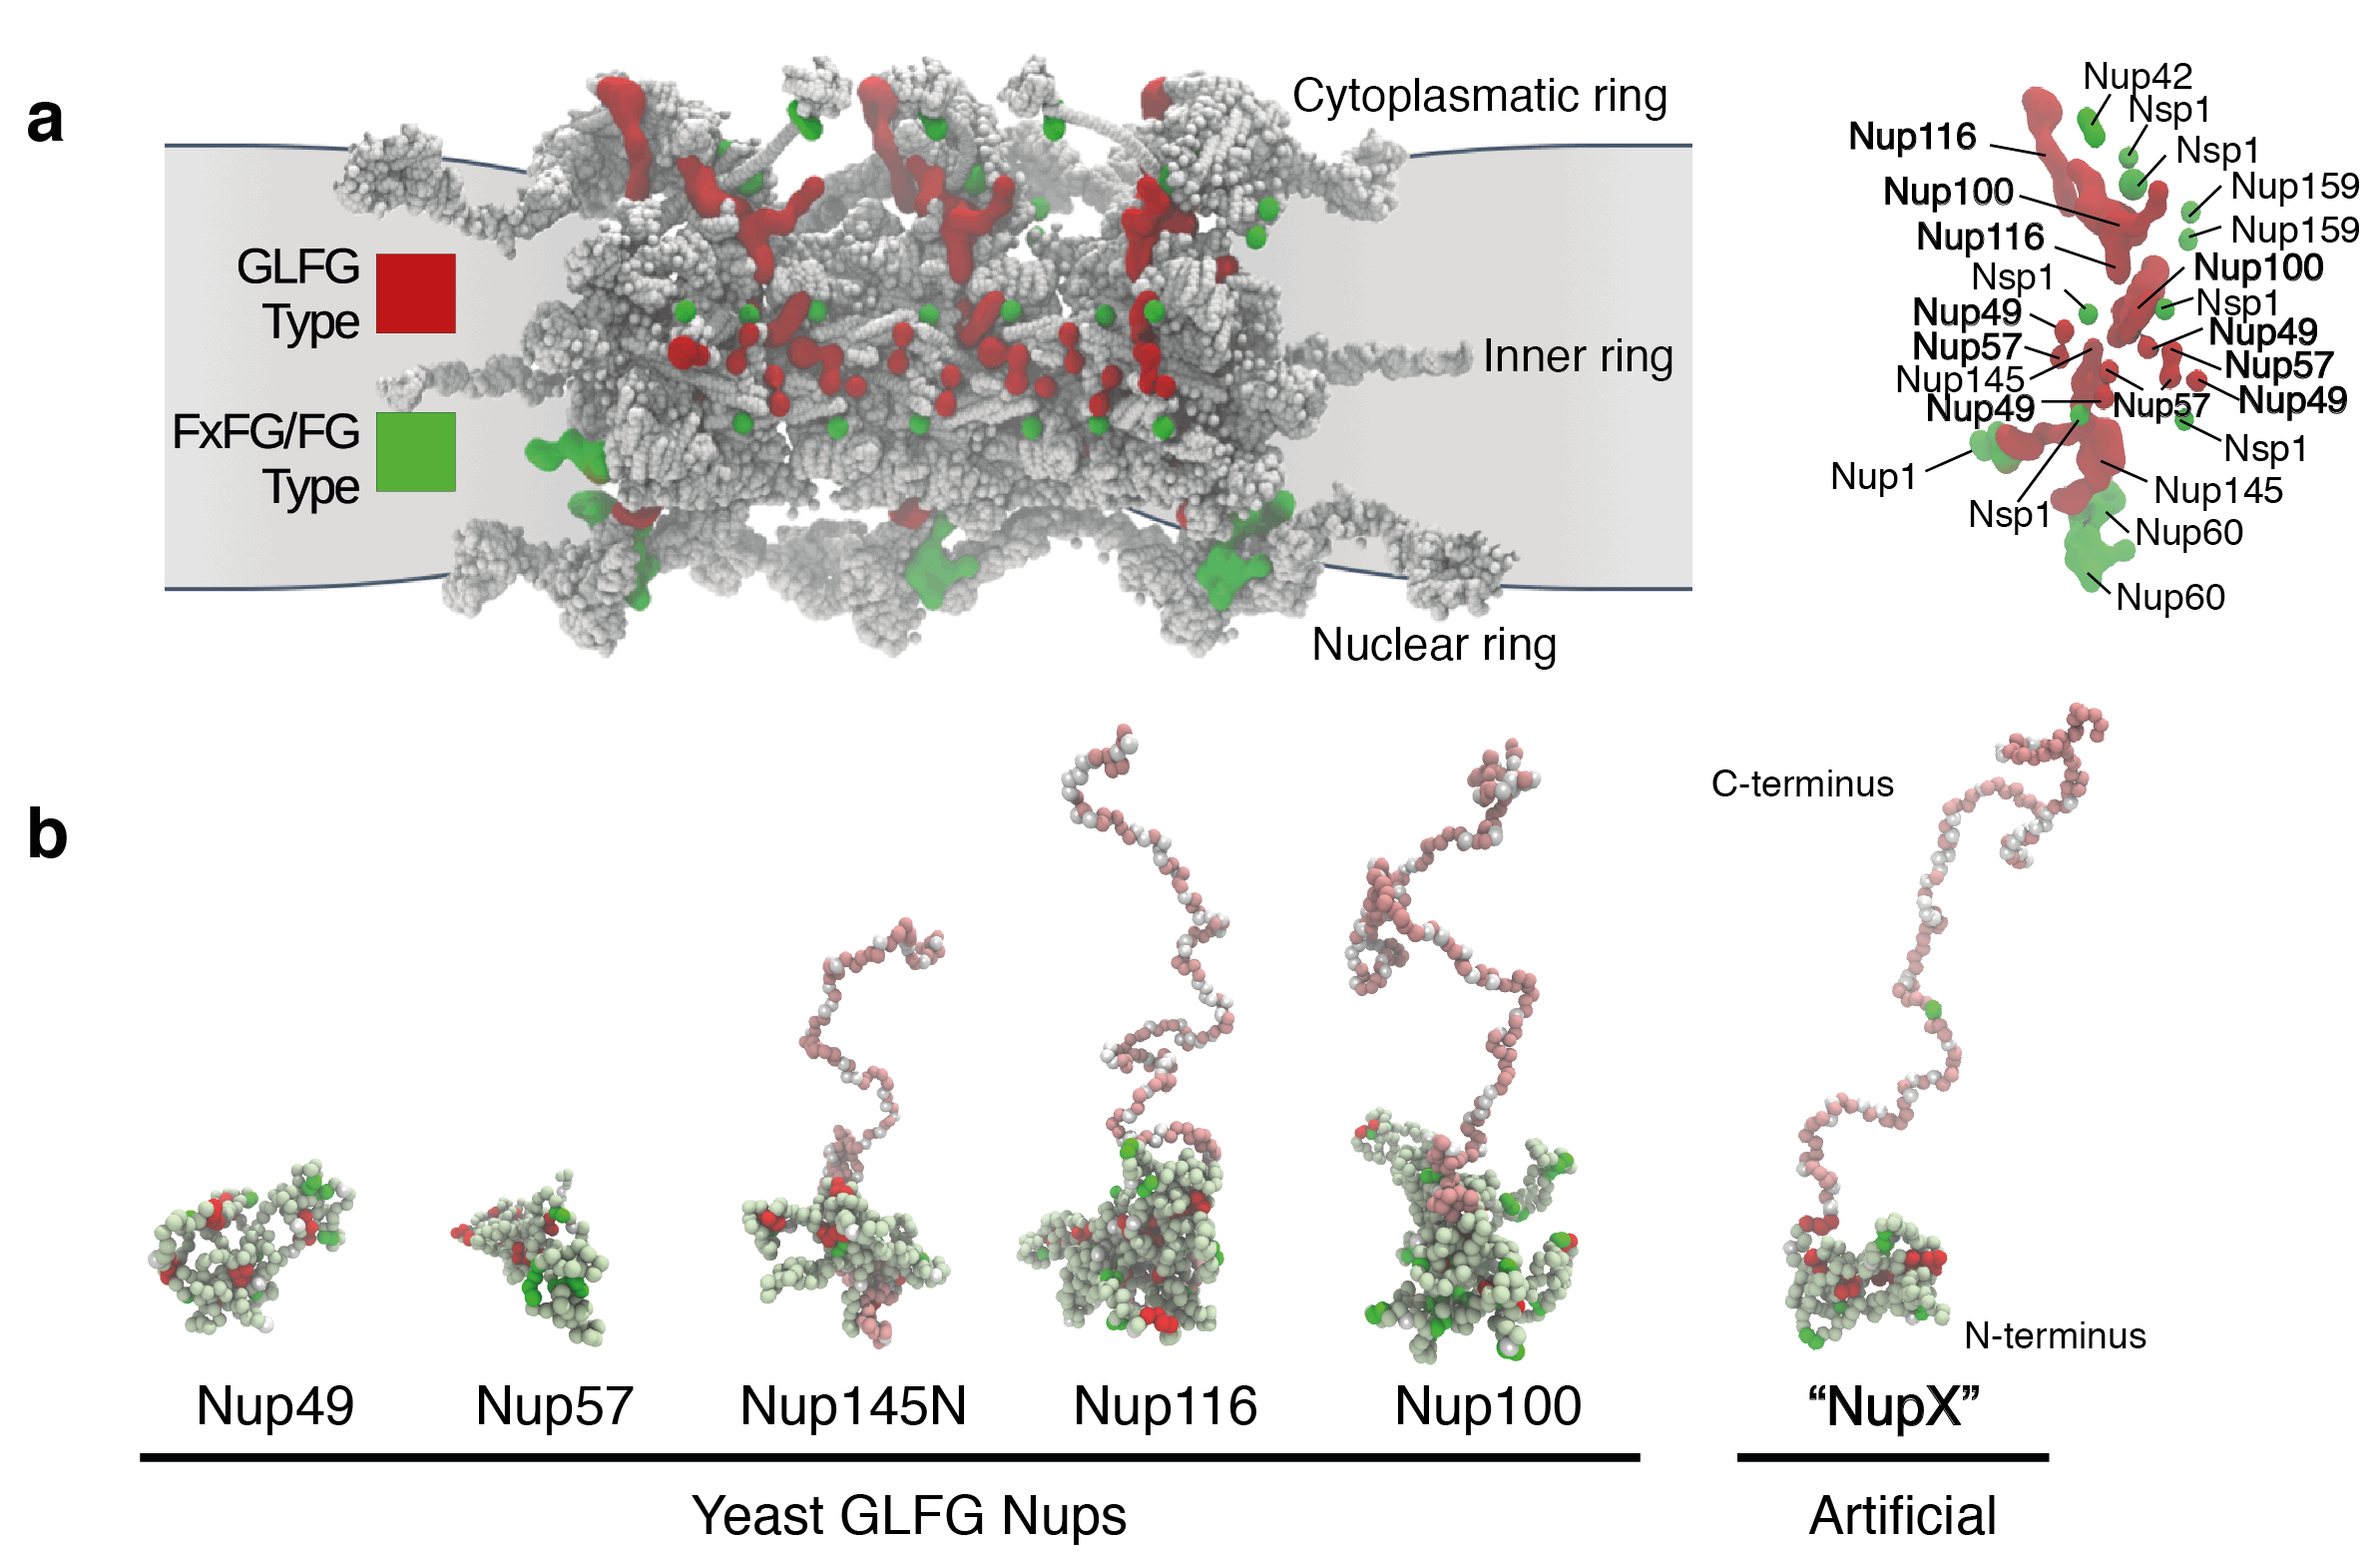
\includegraphics[width=1\linewidth]{figures/Figure4.1.1.png}
	\caption{\emph{De novo} design of an artificial FG-Nup. a, Left: Frontal view on three spokes of the \emph{Saccharomyces cerevisiae} NPC (PDB-DEV, entries 11 and 12, Ref.\cite{Kim2018}) that shows how the GLFG-Nups (red) are predominantly anchored in the inner ring, as opposed to the FxFG/FG-Nups (green). Right: Anchoring points of individual Nups in a single spoke. The GLFG-Nups Nup100, Nup116, Nup49, and Nup57 (red) contribute strongly to the permeability barrier of the NPC3, where Nup100 and Nup116 are known to be indispensable for NPC viability \cite{Adams2016,Strawn2004}. This image and other visualizations of protein structures were rendered using VMD \cite{Humphrey1996}. b, Simulation snapshots of isolated native yeast GLFG-Nups at one amino acid resolution. The conformations of Nup145N, Nup116, Nup100 highlight a bimodality of the Nups \cite{Yamada2010}, with a collapsed and extended domain. FG repeats, GLFG repeats, and charged residues are displayed in bright green, red, and white, respectively. Other amino acids in the cohesive and extended domains are depicted in light green and pink, respectively. NupX adopts the same bimodal conformations as essential GLFG-Nups Nup100 and Nup116. }
\label{fig:fig.4.1.1}	
\end{figure}

\begin{figure}[!htb]
	\centering
	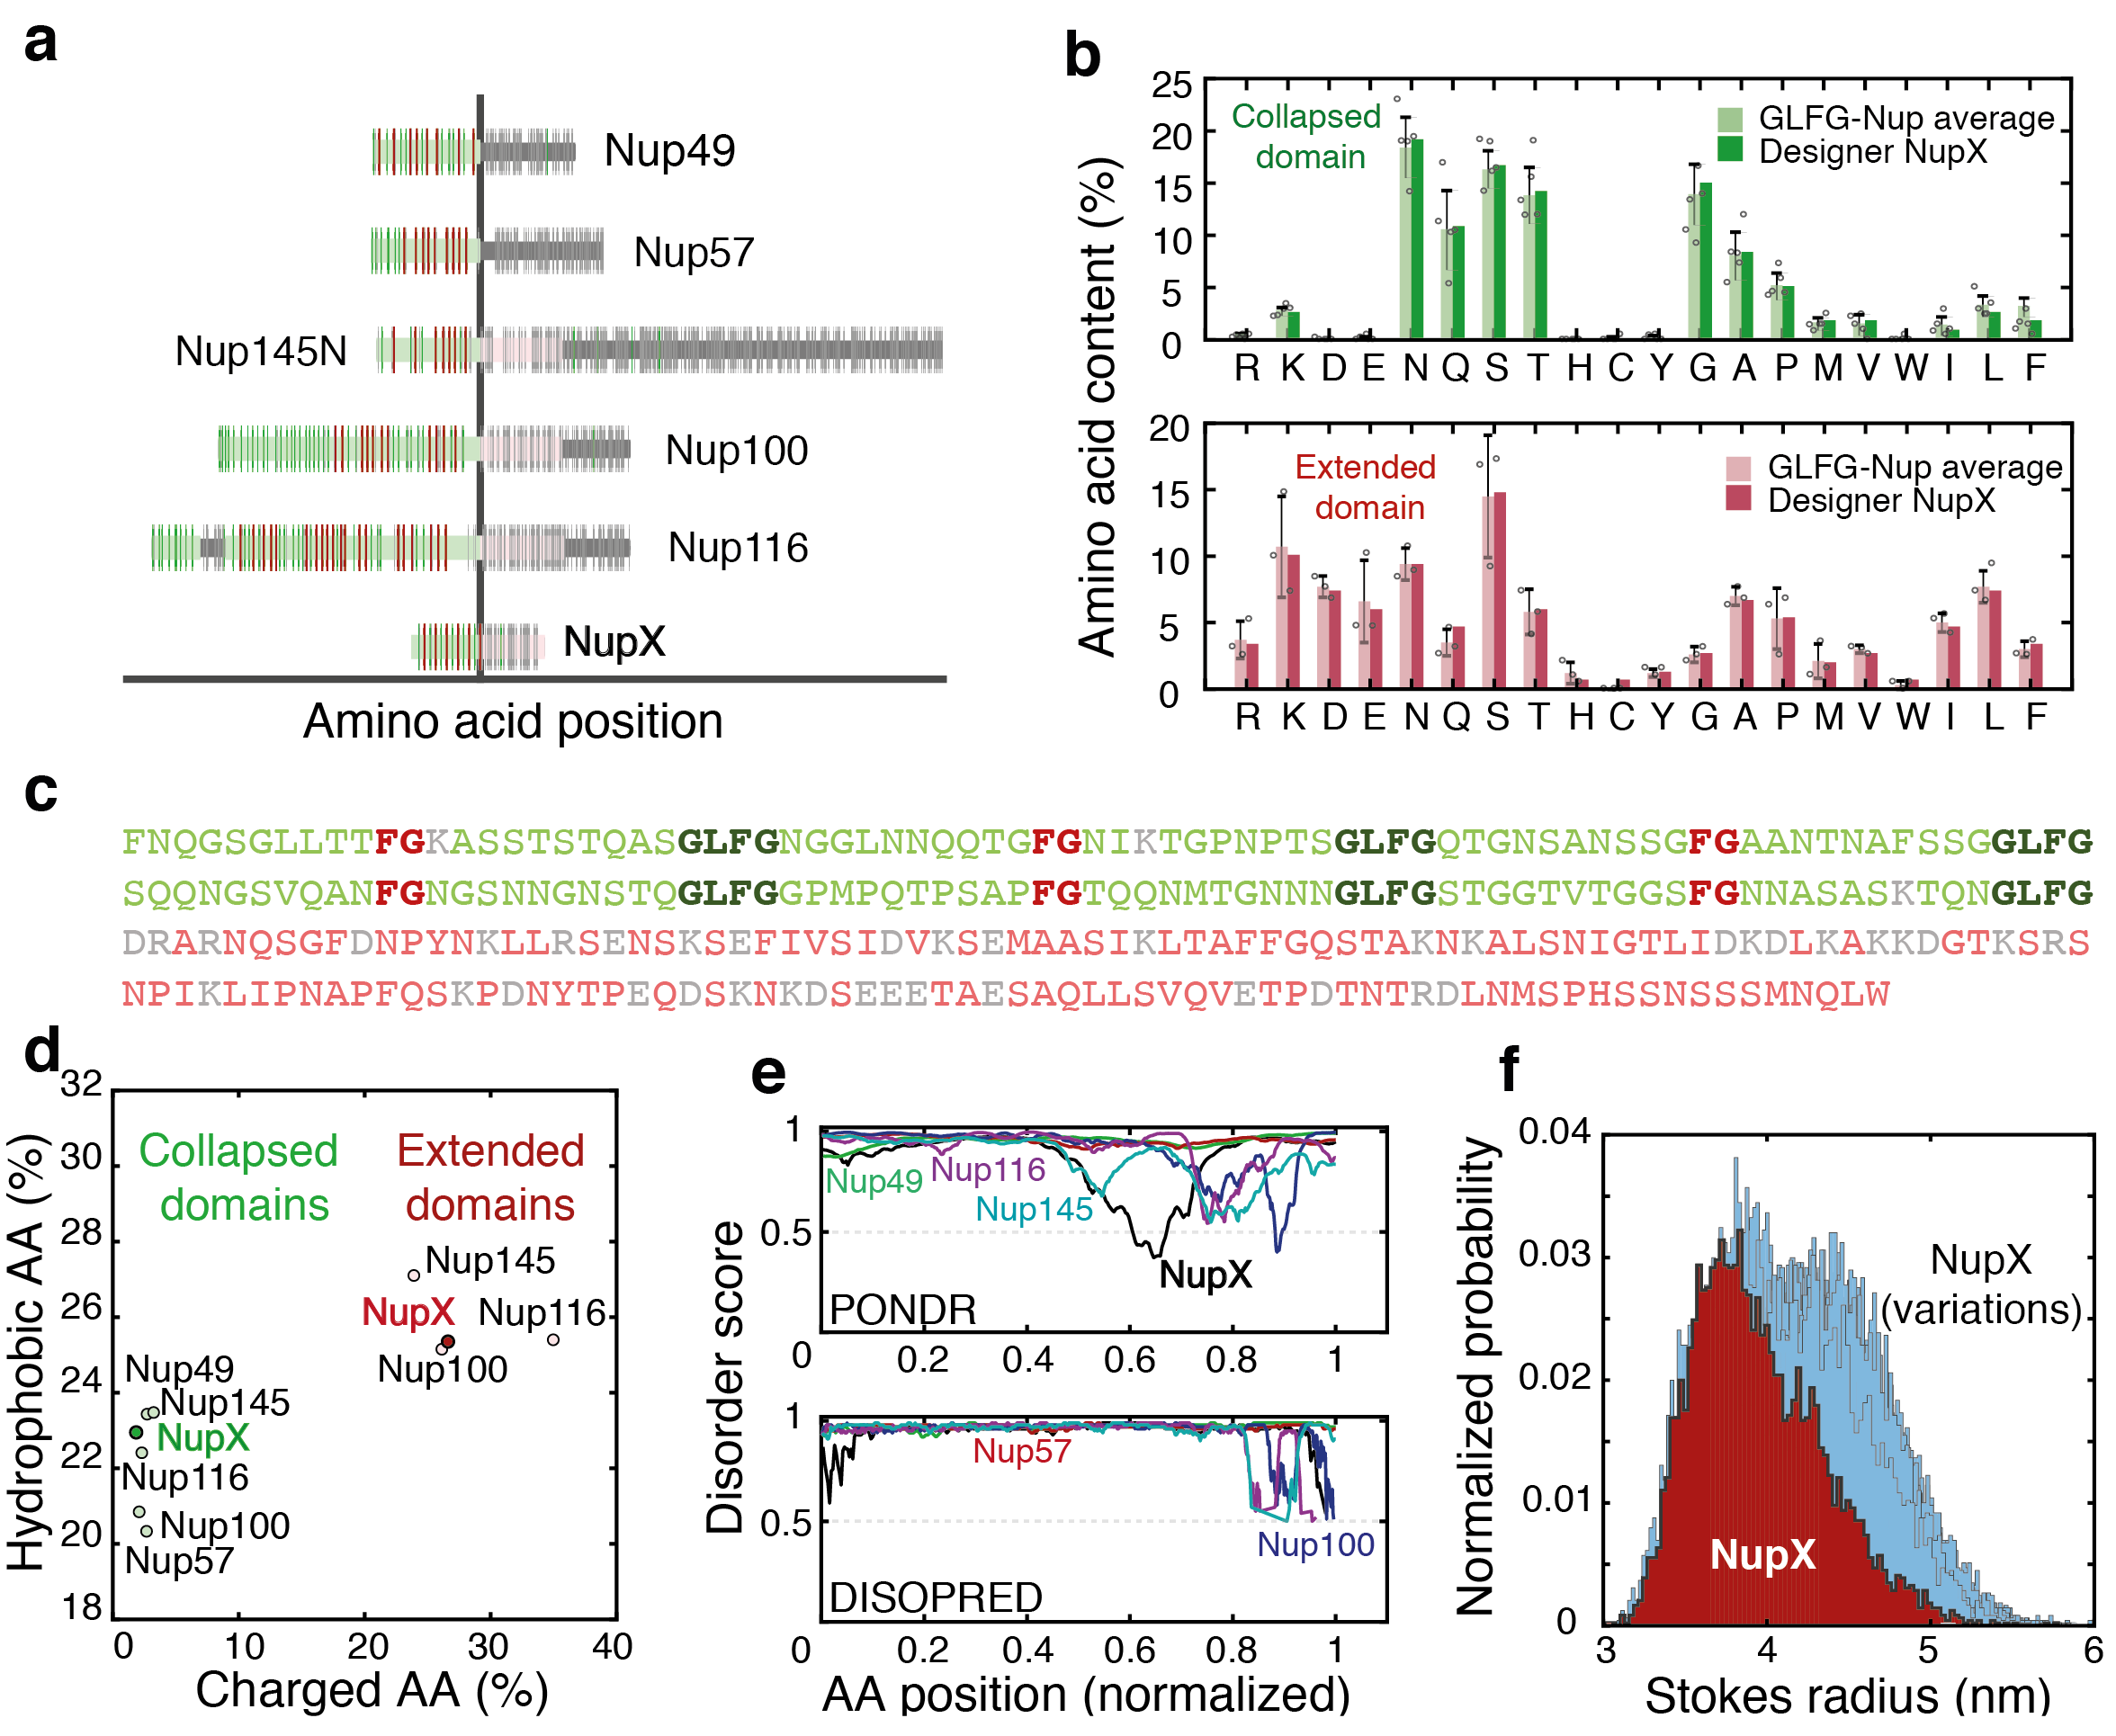
\includegraphics[width=1\linewidth]{figures/Figure4.1.2.png}
	\caption{a, Comparison of the full-length sequences between yeast GLFG-Nups and NupX. Sequence highlights follow the colour-scheme of Fig.\ref{fig:fig.4.1.1}b, folded domains are indicated in dark-grey. b, Amino acid contents of yeast GLFG-Nups (averaged) and NupX for the collapsed (top panel) and extended (bottom panel) domains. Bar heights denote the average amino acid fraction within GLFG-Nup domains, where N=5 (all GLFG-Nups) for the collapsed domain and N=3 (Nup100, Nup116, Nup145) for the extended domain. Error bars indicate standard deviations in the average occurrence of amino acids. FG and GLFG-motifs were excluded from this analysis. c, Sequence of NupX, following the colour scheme of figures \ref{fig:fig.4.1.1}b and panel a. FG and GLFG repeats are spaced by 10 residues in the cohesive domain. d, Charge-and-hydrophobicity plot of NupX and yeast GLFG-Nup domains. For both the collapsed (green shading) and extended (red shading) domains, the charged and hydrophobic amino acid contents of NupX agree with the properties of individual GLFG-Nups. e, Disorder prediction scores for the unfolded domains of GLFG-Nups (coloured lines) and full-length NupX (black curve) from two different predictors (see Materials and Methods). Disorder prediction scores higher than 0.5 (dashed line) count as fully disordered. f, Distribution of Stokes radii from 10 $\mu$s of coarse-grained molecular dynamics simulations for NupX (red) and 25 design variations (light blue). NupX is, on average, slightly more compacted than other design variants.}
	\label{fig:fig.4.1.2}
\end{figure}


We implemented our design rules in a step-wise design process as follows: First, we selected and analysed an appropriate set of native FG-Nups (design rule i), namely GLFG-Nups, which differ from other FG-Nups in terms of the type of FG repeats and the properties of the spacer regions11. The emphasis on GLFG-Nups follows from their localization in the central channel \cite{Kim2018} of the yeast NPC (Figure \ref{fig:fig.4.1.1}a), where they strongly contribute to the nuclear transport selectivity. Indeed, a small subset of GLFG-Nups (\emph{e.g.}, either Nup100 or Nup116 in combination with Nup145N) was shown to be essential and sufficient for cell viability \cite{Adams2016,Strawn2004}. To derive the amino acid content of NupX, we therefore characterized the archetypical GLFG-Nup sequence by determining the amino acid content of the disordered regions of Nup49, Nup57, Nup145N, Nup116, and Nup100 from yeast. Of these, the most essential GLFG-Nups (\emph{i.e.} Nup100, Nup116, and Nup145N) comprise a collapsed domain with a low C/H-ratio and abundance of FG/GLFG repeats, and an extended domain with a high C/H-ratio and absence of FG repeats \cite{Yamada2010}5. This distinction is highlighted in Figures \ref{fig:fig.4.1.1}b,\ref{fig:fig.4.1.2}a, where non-FG/GLFG/charged residues are highlighted in light green and pink for the collapsed and extended domains in respectively – a colouring scheme used throughout this work. The division into two domains of these essential GLFG-Nups led us to phrase design rule ii in our design process of NupX, with each domain comprising $\sim$150 amino acid residues (see Figures \ref{fig:fig.4.1.1}b, \ref{fig:fig.4.1.2}a). Whereas the extended domain of NupX is of quite similar length to the corresponding extended domains of Nup100, Nup116 and Nup145N (190 residues on average), the cohesive domain is notably shorter than the collapsed domains of native GLFG-Nups (390 residues on average).

Assigning the amino acid (AA) content to NupX, as derived from the sequence information of the GLFG-Nups, was performed separately for the two domains: we computed the cumulative amino acid contents (excluding FG and GLFG motifs) for both the collapsed domains of all five GLFG-Nups, and for the extended domains of Nup100, Nup116 and Nup145N (design rule ii). Upon normalizing for the total length of the collapsed or extended domains of all native GLFG-Nups, this analysis resulted in the distributions presented in \ref{fig:fig.4.1.2}b, plotted separately for the collapsed (light green, top) and the extended (light red, bottom) domains. Based on these histograms, we assigned amino acids to the collapsed and extended domains of NupX separately. Following design rule iii, we then placed FG and GLFG repeats in the collapsed domain with a fixed spacer length of 10 AAs. This value was chosen based on the spacer length of $\sim$5-15 AAs in native GLFG-Nups. An analysis of the charged and hydrophobic amino acid content of the domains of NupX and native GLFG-Nups shows that the assigned sequence properties are indeed reproduced by our design method (Figure \ref{fig:fig.4.1.2}d). Finally, the sequences of the collapsed and extended domains of NupX were repetitively shuffled (except for the FG and GLFG motifs that we kept fixed) until a desirable level of disorder was achieved (design rule iv), as predicted by PONDR\cite{Peng2006} and DISOPRED \cite{Jones2015a,Ward2004} (Figure \ref{fig:fig.4.1.2}e). This resulted in the NupX sequence shown in Figure \ref{fig:fig.4.1.2}c. Whereas PONDR predicts one short folded segment between residues 189 and 209 (normalized position of 0.65 in Figure \ref{fig:fig.4.1.2}e), additional structure prediction \cite{Kelley2015} (Materials and Methods) did not yield any high-confidence folded structures for this segment.

To assess the robustness of our design procedure, we tested how permutations of the NupX sequence (which shuffle amino acids while retaining the FG/GLFG sequences and the definition of both domains) affect the Stokes radius $R_s$, as computed from 1-bead-per-amino-acid MD-simulations developed for intrinsically disordered proteins (Figure \ref{fig:fig.4.1.2}f, see Materials and Methods). We found that over 25 different designs for NupX (Table \ref{tab:table4.2}) yielded an average $R_s$ of $4.2\pm 0.2$ nm (errors are S.D.). This is close to the simulated ($3.9\pm 0.4$ nm) and measured ($3.7\pm 1.1$ nm by DLS, Table \ref{tab:table4.1}) $R_s$ value of the NupX protein design (Figure \ref{fig:fig.4.1.2}c).

Summing up, using a minimal set of rules, we designed a NupX protein that incorporates the average properties that characterize GLFG-Nups \cite{Yamada2010,Lim2006}. Moreover, by creating 25 different designs that all showed similar behaviour in our simulations, we showed that the physical properties such as the Stokes radius and the division of NupX into a cohesive and repulsive domain are recovered in a reliable way.


\subsection{QCM-D experiments and MD simulations show selective binding of Kap95 to NupX brushes}

To assess the interaction between NupX and Kap95, we employed a Quartz-Crystal-Micro\-balance with Dissipation monitoring (QCM-D), with gold-coated quartz chips and phosphate-buffered saline (PBS, pH 7.4) as running buffer, unless stated otherwise. First, C-terminus-thiolated NupX molecules were injected into the chamber at a constant flow-rate (20 $\mu$L/min) where they chemically reacted with the gold surface. Binding of NupX to the gold surface could be monitored in real-time by measuring the shift in resonance frequency $\Delta$f of the quartz chip (Figure \ref{fig:fig.4.2}a). We applied the NupX coating by administering a protein concentration ranging from 100 nM to 2 $\mu$M (Figure \ref{fig:fig.4.9}2) until a plateau in the frequency shift was reached, which typically occurred after $\sim$1hr of incubation. To gain insight into the areal mass density of the deposited layers, we employed Surface Plasmon Resonance (SPR) measurements (Figure \ref{fig:fig.4.10}), where we used the same coating protocol for consistency. From these measurements of the areal mass density, we found grafting distances of $7.7\pm 0.5$ nm (mean $\pm$ S.D.) for chips incubated with a 60 nM NupX solution, and $2.91 \pm 0.02$ nm (mean $\pm$ S.D.) for 2 $\mu$M. In determining the grafting density from the areal mass density, we assumed a triangular lattice (since an equilateral triangulated (sometimes also denoted as hexagonal) lattice is the densest type of packing that can be described by a unique length scale that sets the grafting density). Figure \ref{fig:fig.4.2}a shows a typical frequency shift over time for the binding of 1 $\mu$M NupX to a gold surface. After the Nup-layer was formed, a 1-mercapto-11-undecylte-tri(ethyleneglycol) molecule (MUTEG), which is expected to form a $\sim$2 nm thin passivating film \cite{Kapinos2014}, was added to passivate any remaining bare gold that was exposed in between NupX molecules (Figure \ref{fig:fig.4.11}). This minimizes unintentional interactions between Kap95 and gold for subsequent binding experiments (Figure \ref{fig:fig.4.12}) \cite{Kapinos2014,Kapinos2017,Hayama2019}. 



\begin{figure}[H]
	\centering
	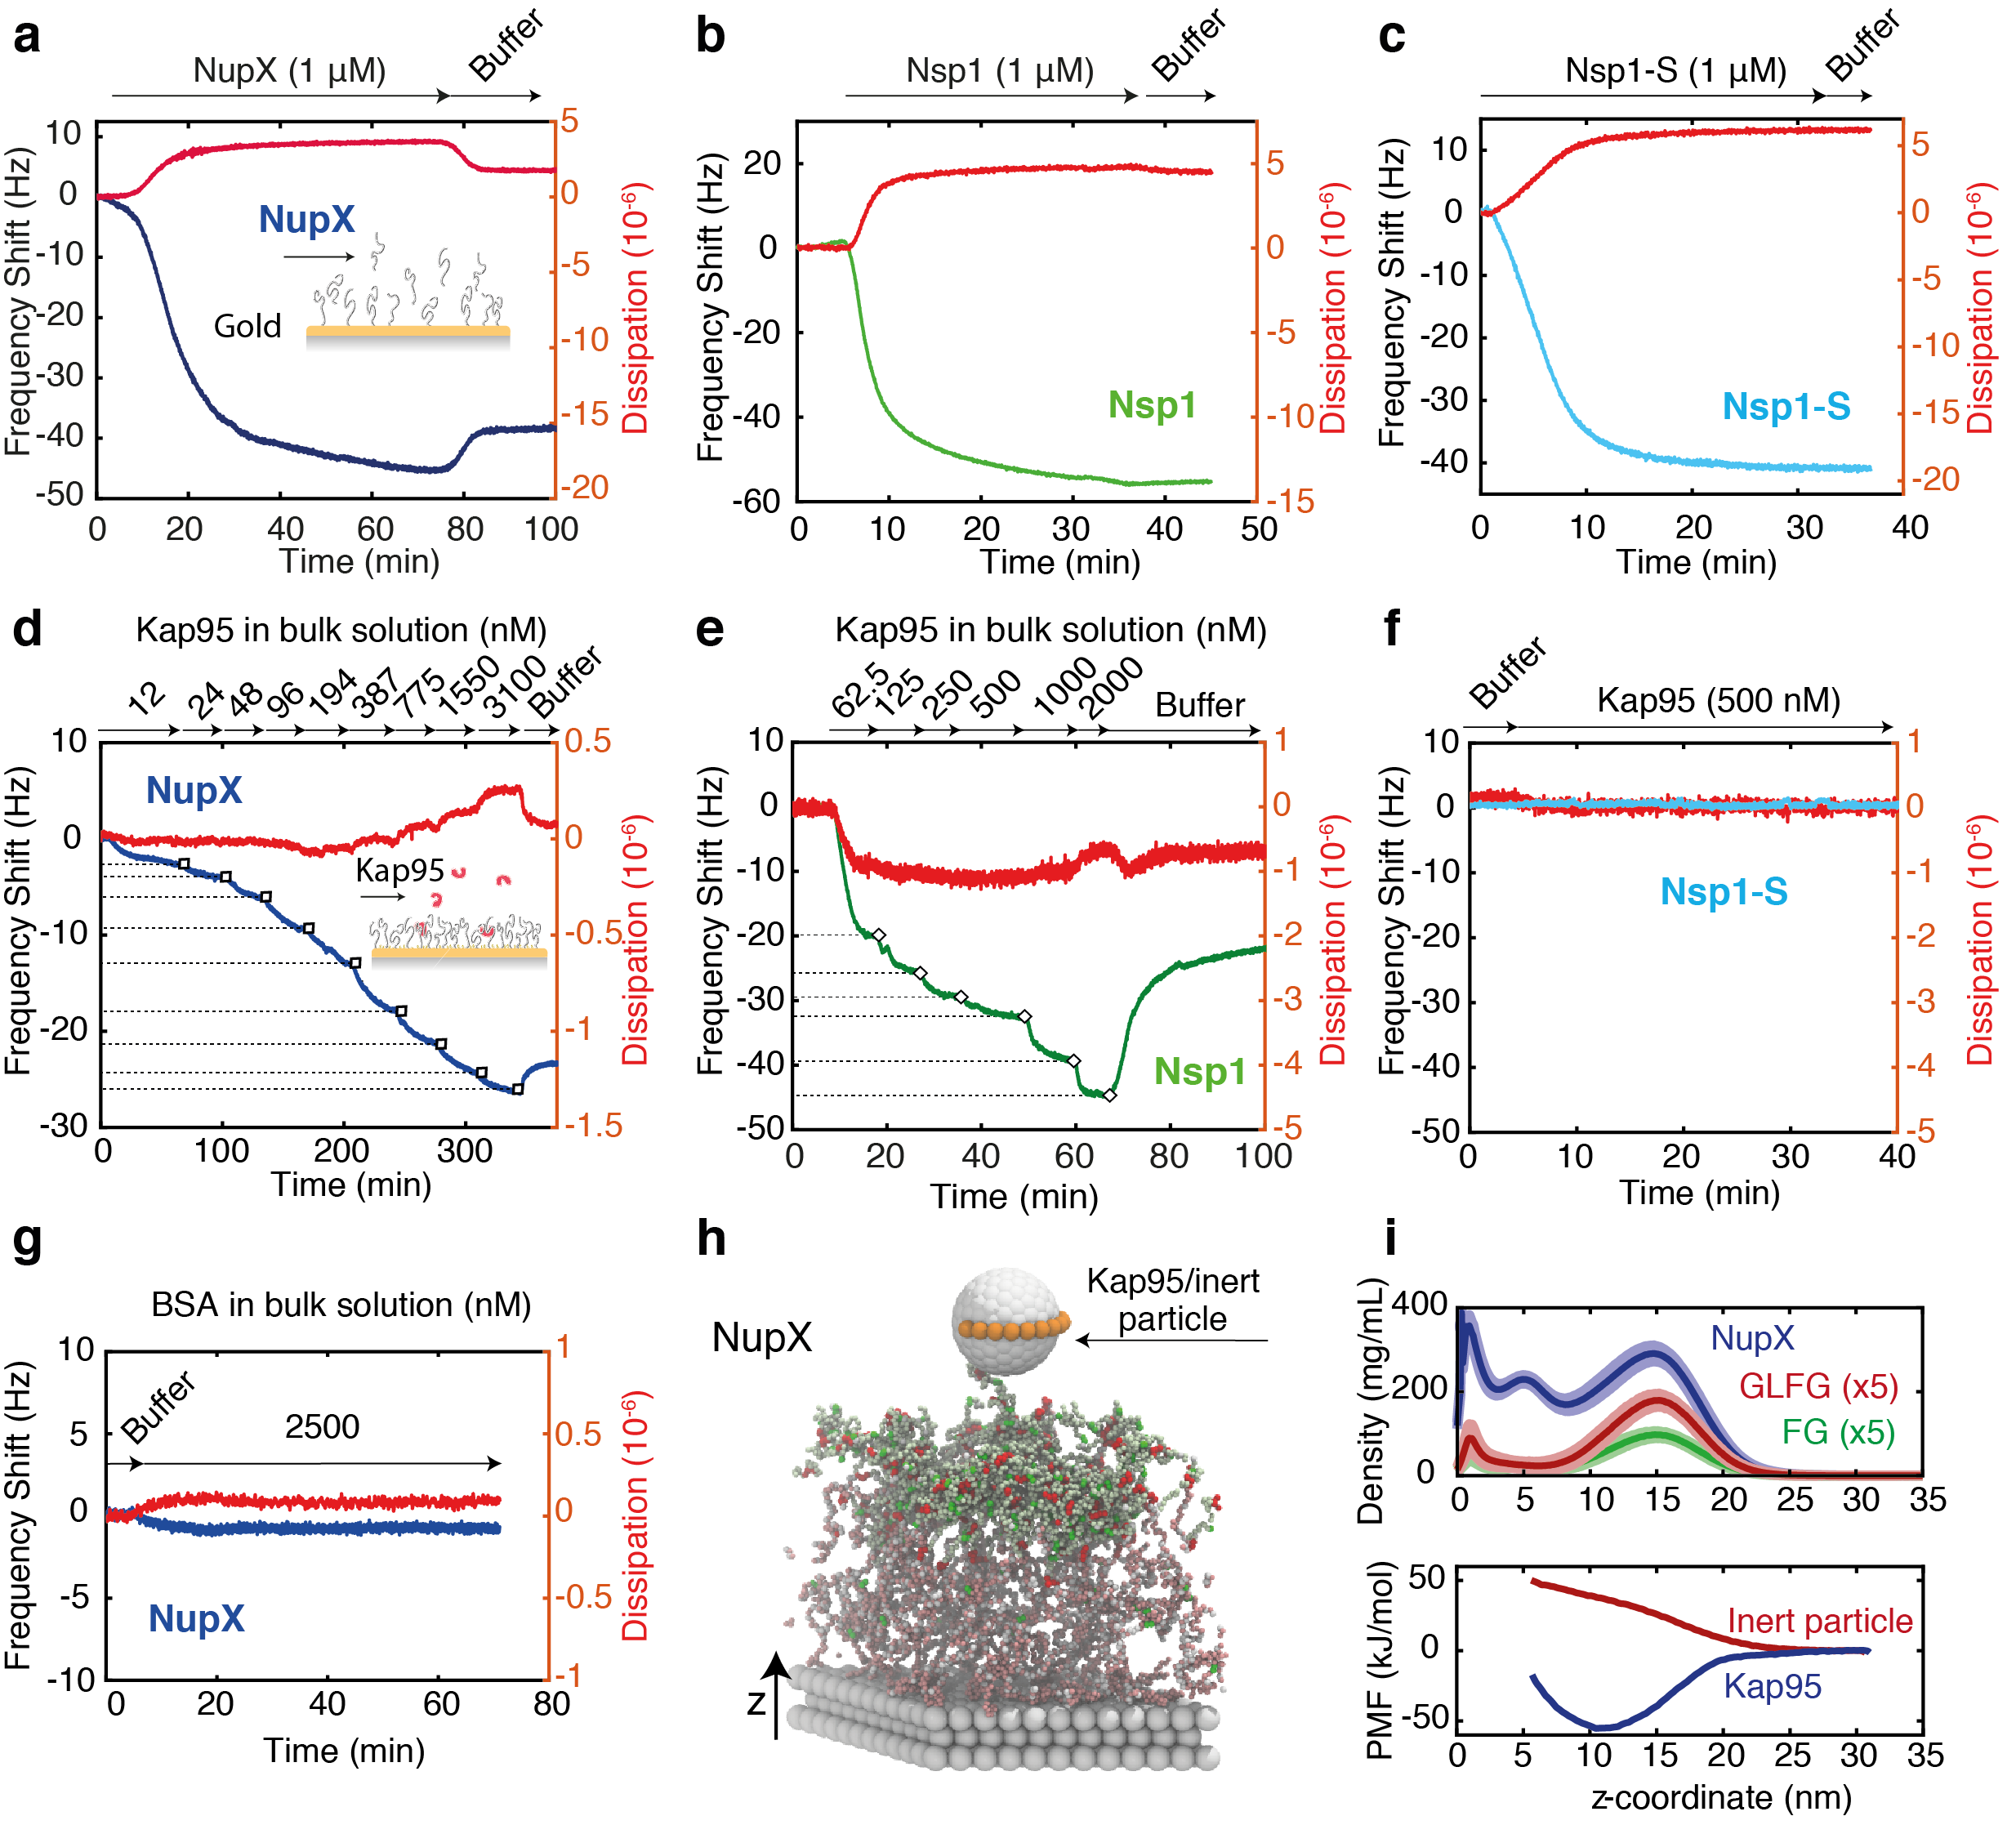
\includegraphics[width=1\linewidth]{figures/Figure4.2.png}
	\caption{Binding affinity of Kap95 to NupX, Nsp1 and Nsp1-S brushes, using QCM-D and MD simulations. a-c, Change in frequency shift upon coating of gold surface with NupX (dark blue), Nsp1 (green), and Nsp1-S (light blue) proteins, respectively, at 1 $\mu$M protein concentration. Red curves indicate the corresponding shift in dissipation. d-f, Change in frequency shift upon titration of Kap95 (with concentration in the range $\sim$10-3000 nM) on NupX (dark blue), Nsp1 (green), and Nsp1-S (light blue) coated surfaces. Numbers indicate the concentration in nM of Kap95 for each titration step. Large changes in frequency shift are observed for NupX and Nsp1, whereas no detectable shift is measured for Nsp1-S. Red curves indicate the corresponding shift in dissipation. g, Frequency (dark blue) and dissipation (red) shift upon adsorption of 2.5 $\mu$M BSA onto the NupX-coated sensor. h, Side-view snapshot of the umbrella sampling simulation setup for a NupX brush with 4.0 nm grafting distance, where a model Kap95 particle (8.5 nm diameter grey sphere with binding sites depicted in brown) or inert particle (7.5 nm diameter, not shown) is restrained along different $z$-coordinates. Scaffold beads are shown in grey, NupX proteins follow the same colour scheme as presented in Figure \ref{fig:fig.4.1.1}b. i, Top panel: Time and laterally averaged protein density distributions for the NupX brushes (blue) and for the FG-motifs (green) and GLFG-motifs (red) present inside the NupX brushes with a grafting distance of 4.0 nm. The density profiles of the GLFG and FG motifs within the NupX brush are multiplied by 5 for clarity. Dark central lines and light shades indicate the mean and standard deviation in density profiles, respectively. These measures were obtained by averaging over the density profiles of trajectory windows 50 ns in length (N=60).  High-density regions (up to almost 400 mg/mL) form near the attachment sites ($z=0$ to 2 nm) and near the free surface of the brush layer (at z $\sim$15 nm). FG and GLFG-motifs predominantly localize near the free surface of the brush. Bottom: Free-energy profiles (PMF-curves) of the center of mass of the 8.5 nm-sized model Kap95 (blue) and inert particle (red) along the $z$-coordinate, where $z=0$ coincides with the substrate. The difference in sign between the PMF-curves of both particles indicates a strong preferential adsorption of the model Kap95 to NupX brushes and a repulsive interaction with the inert particle.}
	\label{fig:fig.4.2}	
\end{figure}


After thus setting up a NupX-coated layer, we flushed in Kap95 at stepwise increasing concentrations ($\sim$10-3000 nM, Figure \ref{fig:fig.4.2}d) and monitored binding to the NupX-coated surface. We observed a clear concentration-dependent amount of Kap95 molecules bound to the NupX brush. For reference, we repeated the experiment on brushes of Nsp1 (a native FG-Nup from yeast), as well as Nsp1-S, a Nsp1-mutant where the hydrophobic amino acids F, I, L, V are replaced by the hydrophilic amino acid Serine (S) (Figure \ref{fig:fig.4.2}b,c). The latter was employed as a negative control since it is expected to not bind Kap95 due to the lack of FG repeats \cite{Frey2006,Frey2007}. Gold surfaces coated with Nsp1 or Nsp1-S were characterized with SPR under similar coating conditions as for QCM-D, yielding grafting distances of $4.9\pm0.1$ nm for Nsp1 and $5.8\pm0.4$ nm for Nsp1-S. Upon flushing Kap95, we found, consistent with previous studies \cite{Eisele2010a,Hayama2019}, a concentration-dependent adsorption to Nsp1 brushes (Figure \ref{fig:fig.4.2}e), whereas we did not observe any detectable interaction between Kap95 and Nsp1-S (Figure \ref{fig:fig.4.2}f). The latter is consistent with the lack of FG repeats in the Nsp1-S sequence which makes the Nsp1-S film devoid of binding sites for Kap95. We note that non-linear effects, \emph{e.g.}, coverage-dependent changes in water entrapment within the layer \cite{Reviakine2011}, as well as mass transport limitations inherent to the QCM-D technique \cite{Hayama2019} are likely to affect the observed binding kinetics, which, together with a relatively slow dissociation of Kap95 from both the NupX and Nsp1 brushes, lead us to refrain from extracting a dissociation constant. Adsorbed molecules could be completely removed upon flushing 0.2 M NaOH however (Figure \ref{fig:fig.4.13}). Finally, we investigated whether the inert molecule BSA could bind to the NupX brush. Upon flushing 2.5 $\mu$M of BSA (Figure \ref{fig:fig.4.2}g) we did not observe any appreciable change in the resonance frequency, indicating that the NupX brush efficiently excludes these inert molecules. This measurement was repeated for all the grafting conditions used in this study (Figure \ref{fig:fig.4.14}) showing that BSA did not produce any detectable shift in frequency, while Kap95 showed clear binding to the NupX films. Importantly, the data show that the NupX brush selectively interacts with Kap95 over a range of grafting densities.


In order to study the morphology and physical properties of NupX brushes at the microscopic level, we employed coarse-grained molecular dynamics (MD) simulations (see Materials and Methods), which resolved the density distribution within the NupX brush layer and the preferential adsorption of Kap95 over inert molecules of similar size such as BSA. 36 NupX proteins were tethered on a triangular lattice with a fixed spacing of 4.0 nm (Figure \ref{fig:fig.4.2}h) or 5.7 nm (Figure \ref{fig:fig.4.18}), well in the range of grafting distances from 2.9 nm to 7.7 nm as measured by SPR. Averaged over a simulation time of 3 $\mu$s, we found that the NupX brushes with a 4.0 nm grafting distance form a laterally homogeneous meshwork with densities ranging from $\sim$400 mg/mL near the substrate to around $\sim$200 mg/mL  in the central region and to $\sim$300 mg/mL near the free surface of the brush (Figure \ref{fig:fig.4.2}i, top panel). The interface near the free surface of the brush contains the highest relative concentration of FG and GLFG motifs (see Figure \ref{fig:fig.4.2}i, top panel). Notably, the protein density throughout the brush is of the same order of magnitude as the density obtained in simulations of the yeast NPC \cite{Ghavami2014}. Upon increase of the grafting distance to 5.7 nm, we find that the NupX brush attains different and less dense conformations: the density profile plateaus at a value of 170 mg/mL and slowly decays without showing a peak density near the free surface of the brush (Figure \ref{fig:fig.4.18}). We translated our density profiles into height estimates in a similar fashion as other computation efforts on FG-Nup brushes \cite{Zahn2016,Davis2020}. We consider the $z$-coordinates at which 90\% of the protein mass is incorporated as the effective brush heights. This approach yields brush heights of 12 and 18 nm for the NupX brushes with 5.7 and 4.0 nm grafting distances, respectively. These values coincide quite well with the inflection point of the decaying tail of the density profiles in Figures \ref{fig:fig.4.2}l and Figure \ref{fig:fig.4.18}. 


The simulated density profiles yield notably higher brushes than expected from the Sauerbrey equation: For example, assuming a density of the hydrated brush of $\sim$1.05 g/mL45, one can estimate a brush height of 6.4 nm for the NupX brush in Figure \ref{fig:fig.4.2}a (that was incubated at 1 $\mu$M, which we expect to have a grafting distance at the higher end of the values used in our simulations). Importantly, however, the Sauerbrey equation does not account for viscoelastic effects and only provides a lower limit to the brush height \cite{Reviakine2011}. Indeed, given the dissipation-to-frequency ratio of $\sim0.045\times 10^{-6}$ Hz\textsuperscript{-1} (Figure \ref{fig:fig.4.16}), one expects that the actual experimental brush height will be larger than 6.4 nm, an effect also seen in other QCM-D studies of FG-Nups \cite{Eisele2010a,Eisele2012}. Notably, a quantitative difference between the NupX brush height estimations of the computational and experimental results does not affect the major conclusions of the study, namely the selective transport across biomimetic nanopores with a rationally designed artificial FG-Nup and the selective binding of Kap95 over BSA to NupX.


To assess the selective properties of the NupX brushes, we performed umbrella sampling simulations of the adsorption of Kap95 and an inert molecule to NupX brushes (Materials and Methods), again for two grafting densities of 4 nm and 5.7 nm. We modelled Kap95 (Figure \ref{fig:fig.4.19}) as an 8.5 nm sized sterically repulsive (\emph{i.e.}, modelling only repulsive, excluded volume interactions) particle with 10 hydrophobic binding sites \cite{Ghavami2016,Ananth2018,Isgro2005,Tagliazucchi2013} and a total net charge similar to that of Kap95 ($–$43e).  The inert molecule was modelled as a sterically inert spherical particle of 7.5 nm diameter \cite{Timney2016}. We obtained  potential-of-mean-force (PMF) curves associated with the adsorption of Kap95 and inert particles by means of the weighted histogram analysis method (WHAM)\cite{Hub2010}. We found that for the dense brush (4.0 nm grafting density), a significant ($–52$ kJ/mol) negative free energy is associated with the entry of Kap95 in the NupX brush, as is visible in Figure \ref{fig:fig.4.2}i (bottom panel). By contrast, the PMF curve of the inert particle steeply increased when the protein entered into the NupX meshwork, showing that adsorption of non-specific proteins of comparable size as Kap95 will not occur. The large free energy differences between Kap95 (corresponding to $\sim$nM binding affinity) and inert particle adsorption qualitatively support the experimental findings. When increasing the grafting distance to 5.7 nm, the inert particle and Kap95 protein are repelled and adsorbed less strongly ($\mu$M binding affinity, similar to other in vitro works \cite{Wagner2015,Kapinos2017}), respectively (Figure \ref{fig:fig.4.18}). The data indicate that dense brushes bind more strongly to Kap95 and that selectivity is maintained for less densely coated NupX brushes, which is in line with our experimental observation of selective adsorption in chips coated with NupX brushes of varying grafting densities (Figure \ref{fig:fig.4.14}). 



\subsection{Single-molecule translocation experiments with NupX-coated nanopores demonstrate selectivity }

In order to test whether our synthetic FG-Nup do indeed form a transport barrier that mimics the selective properties of the NPC, we performed electrophysiological experiments on biomimetic nanopores \cite{Kowalczyk2011a,Ananth2018}. These NPC mimics were built by tethering NupX proteins to the inner walls of a solid-state SiN\textsubscript{x} nanopore \cite{Dekker2007} using Self-Assembled-Monolayer (SAM) chemistry (details in Materials and Methods). Solid-state nanopores of 10-60 nm in diameter were fabricated onto a glass-supported \cite{Balan2015} SiN\textsubscript{x} free-standing membrane by means of TEM drilling. A buffer with 150 mM KCl, 10 mM Tris, 1 mM EDTA, at pH 7.5 was used to measure the ionic conductance through the pores, while retaining near-physiological conditions. Coating bare SiN\textsubscript{x} pores with NupX yielded a significant decrease in conductance (\emph{e.g.} $\sim$50\% for $\sim$30 nm diameter SiN\textsubscript{x} pores) of the bare-pore values, as estimated by measuring the through-pore ionic current before and after the functionalization (Figure \ref{fig:fig.4.20}). Additionally, the current-voltage characteristic in the $\pm$200 mV range (Figure \ref{fig:fig.4.20}) is linear both for the bare and NupX-coated pores, indicating that the NupX meshwork is not affected by the applied electric field at the 100 mV operating bias. To obtain more information on the NupX-coating process of our SiN\textsubscript{x} pores, we repeated the same functionalization procedure on silica-coated SPR chips (Figure \ref{fig:fig.4.10}), where APTES, Sulfo-SMCC, and NupX coatings were independently characterized using the same coating protocol as for the SiN\textsubscript{x} nanopores, for consistency. From these experiments, we estimate an average grafting distance of $5.4\pm1.1$ nm between adjacent NupX molecules. Measurements of the ionic current through NupX-coated pores revealed a higher 1/f noise in the current (Figure \ref{fig:fig.4.21}) compared to bare pores, which we attribute to random conformational fluctuations of the Nups within the pore volume and access region \cite{Kowalczyk2011b,Fragasso2019}, similar to findings from previous studies on biomimetic nanopores \cite{Kowalczyk2011a,Ananth2018}. 


To test the selective behaviour of the biomimetic nanopore, we measured translocation rates of Kap95 and BSA through bare pores of $\sim$30-35 nm in diameter (Figure \ref{fig:fig.4.3}a). Figure \ref{fig:fig.4.3}c shows examples of raw traces recorded for a 30 nm pore under 100 mV applied bias, when either only buffer (top), 450 nM Kap95 (middle), or 2.8 $\mu$M BSA (bottom) were added to the cis-chamber. As expected, we observed transient dips in the current through the bare pore upon injection of the proteins, which we attribute to single-molecule translocations of the analyte molecules. As is typical in nanopore experiments, translocation events yield current blockades with a characteristic amplitude and dwell time, where the former relates to the size of the molecule occupying the pore and the latter generally depends on specific interaction between the translocating molecule and the pore wall\cite{Varongchayakul2018}. Next, we repeated the experiment under identical conditions on the same pore after coating with NupX took place (Figure \ref{fig:fig.4.3}b). Examples of typical raw traces are shown in Figure \ref{fig:fig.4.3}d. Strikingly, Kap95 molecules could still translocate efficiently through the NupX-coated pore, whereas BSA molecules were practically blocked from transport. 



\begin{figure}[!htb]
	\centering
	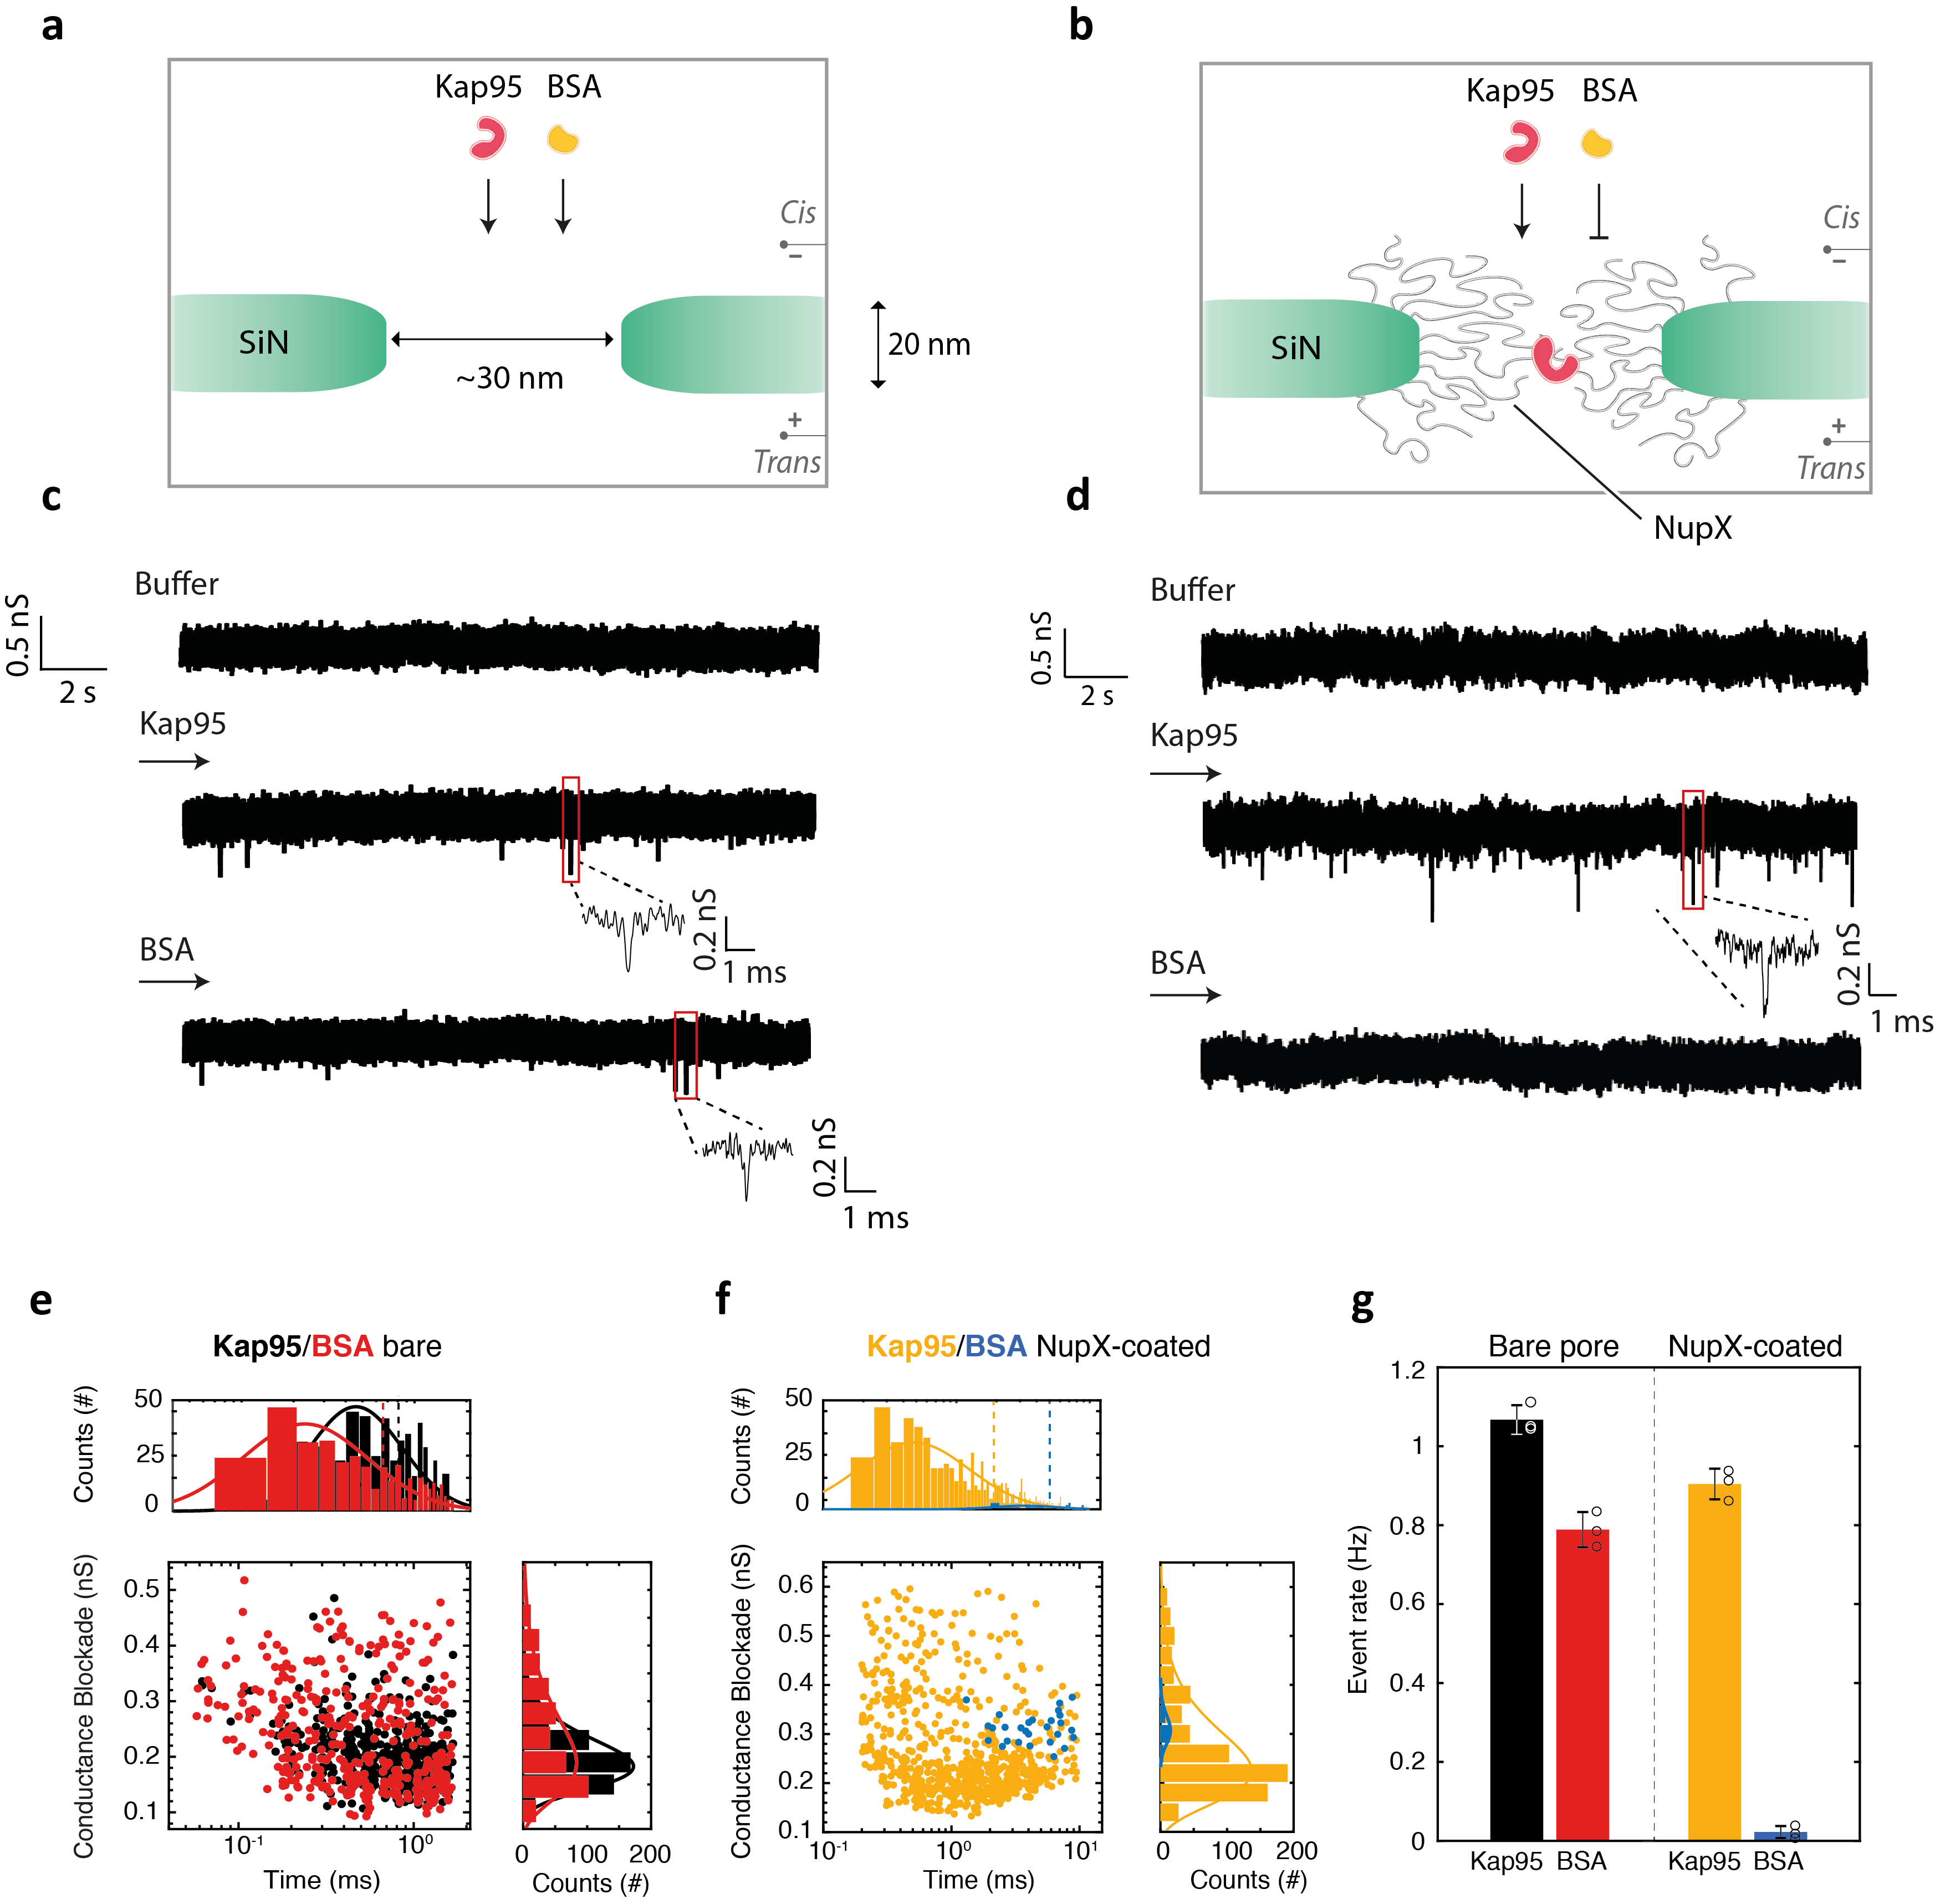
\includegraphics[width=1\linewidth]{figures/Figure4.3.png}
	\caption{Electrical measurements on NupX-coated solid-state nanopores. a-b, Schematic of the nanopore system before (a) and after (b) NupX functionalization. c-d, Examples of raw current traces through bare (c) and NupX-coated (d) pores, recorded under 100 mV applied bias for different analyte conditions. Current traces are recorded in the presence of buffer only (top), upon addition of 450 nM Kap95 (middle), and 2.8 $\mu$M BSA (bottom). Traces were filtered at 5 kHz. e, Scatter plot showing conductance blockades and dwell time distributions of translocation events of the analytes Kap95 (black, N=506) and BSA (red, N=387) through a bare 30 nm pore, recorded over the same time interval. f, Scatter plot showing conductance blockades and dwell time distributions of translocation events of the analytes Kap95 (yellow, N=686) and BSA (blue, N=28) through a NupX-coated 30 nm pore, recorded over the same time interval. Top and right panels in e and f show lognormal fits to the distribution of dwell times and conductance blockades, respectively. Dashed vertical lines in top panels indicate the mean values for the dwell time distributions. g, Average event rate of translocations for Kap95 through a bare pore (black), BSA through a bare pore (red), Kap95 through a NupX-coated pore (yellow), and BSA through a NupX-coated pore (blue). Error bars indicate standard deviations from independent measurements (circles) on three different pores, N=3.}
	\label{fig:fig.4.3}	
\end{figure}

Figures \ref{fig:fig.4.3}e-f show scatter plots of the event distributions, where the conductance blockade is plotted against dwell time for all translocation events. For the bare pore, we observe similar average amplitudes of $0.24\pm0.09$ nS and $0.20\pm0.05$ nS (errors are s.d.) for BSA and Kap95, respectively. For the NupX-coated pore, we found slightly larger but again mutually similar event amplitudes of $0.31\pm0.03$ nS and $0.27\pm0.03$ nS for BSA and Kap95, respectively. We found comparable translocation times through the bare pore of $0.66\pm0.03$ ms and $0.81\pm0.02$ ms (errors are s.e.m) for BSA and Kap95, respectively. For the coated pore, however, we measured longer dwell times of $5.0\pm0.5$ ms and $1.9\pm0.1$ ms for BSA and Kap95, respectively, which indicates that the presence of the NupX molecules in the pore significantly slows down the translocation process of the passing molecules. Notably, BSA molecules were slower in translocating through the coated pore as compared to Kap95, which we attribute to the lower affinity between BSA and the NupX mesh as compared to Kap95. The transient and multivalent interactions between Kap95 and the FG-repeats in the NupX meshwork lead to a reduced energy barrier as compared to BSA permeation, which may explain the observed differences in dwelling times\cite{Timney2016}. Repeating the same experiment on a larger 60 nm NupX-coated pore (Figure \ref{fig:fig.4.22}) yielded selective pores with faster translocations for both Kap95 ($0.65\pm0.05$ ms) and BSA ($1.6\pm1.3$ ms), consistent with the presence of an open central channel. Smaller pores ($<25$ nm) did not result in any detectable signal for either Kap95 or BSA, due to the poor signal-to-noise ratio attainable at such low conductances.


Most importantly, these data clearly show selectivity of the biomimetic pores. Figure \ref{fig:fig.4.3}g compares the event rate of translocations for Kap95 and BSA through bare and NupX-coated pores under 100 mV applied bias. Event rates were $0.7\pm0.04$ Hz and $1.10 \pm0.04$ Hz (N=3 different nanopores; errors are s.d.) for BSA and Kap95 through the bare pore, respectively, whereas upon coating the pore with NupX, the event rates changed to $0.02\pm0.02$ Hz and $0.90\pm0.04$ Hz (N=3 different nanopores) for BSA and Kap95, respectively. The sharp decrease in event rate for BSA upon NupX coating of the pores indicates that BSA molecules are strongly hindered by the NupX meshwork formed inside the pore. In contrast, the transport rate of Kap95 through the coated pore is nearly unaffected when compared to the bare pore. From these experiments, we conclude that the user-defined NupX does impart a selective barrier, very similar to native FG-Nups \cite{Jovanovic-Talisman2009,Kowalczyk2011a,Ananth2018}, by allowing efficient transportation of Kap95 while hindering the passage of BSA.





\subsection{MD simulations of NupX-lined nanopores reveal their protein distribution and selectivity}

We used coarse-grained MD simulations (Materials and Methods) to understand the selective properties of NupX-lined nanopores as obtained in our experiments. The 20 nm height of these nanopores is the same as the SiN\textsubscript{x} membrane thickness, while we vary the diameter from 15 to 70 nm. Multiple copies of NupX are tethered to the nanopore lumen by their C-terminal domain in an equilateral triangular lattice with a spacing of 5.5 nm, based on estimates obtained from the SPR experiments (Figure \ref{fig:fig.4.10}, Materials and Methods). We note that the geometrical confinement by the nanopore may affect the grafting distance on the concavely curved interior pore wall (parallel to the pore axis) as compared to the planar geometry \cite{Koutsioubas2009}. Based on 6 $\mu$s of coarse-grained MD simulations, we obtained the protein density distribution in the ($r$,$z$)-plane (averaged over time and angle $\theta$) within a NupX-lined nanopore of 30 nm in diameter (Figure \ref{fig:fig.4.4.1}b), similar in size as the translocation experiments. 


\begin{figure}[!htb]
	\centering
	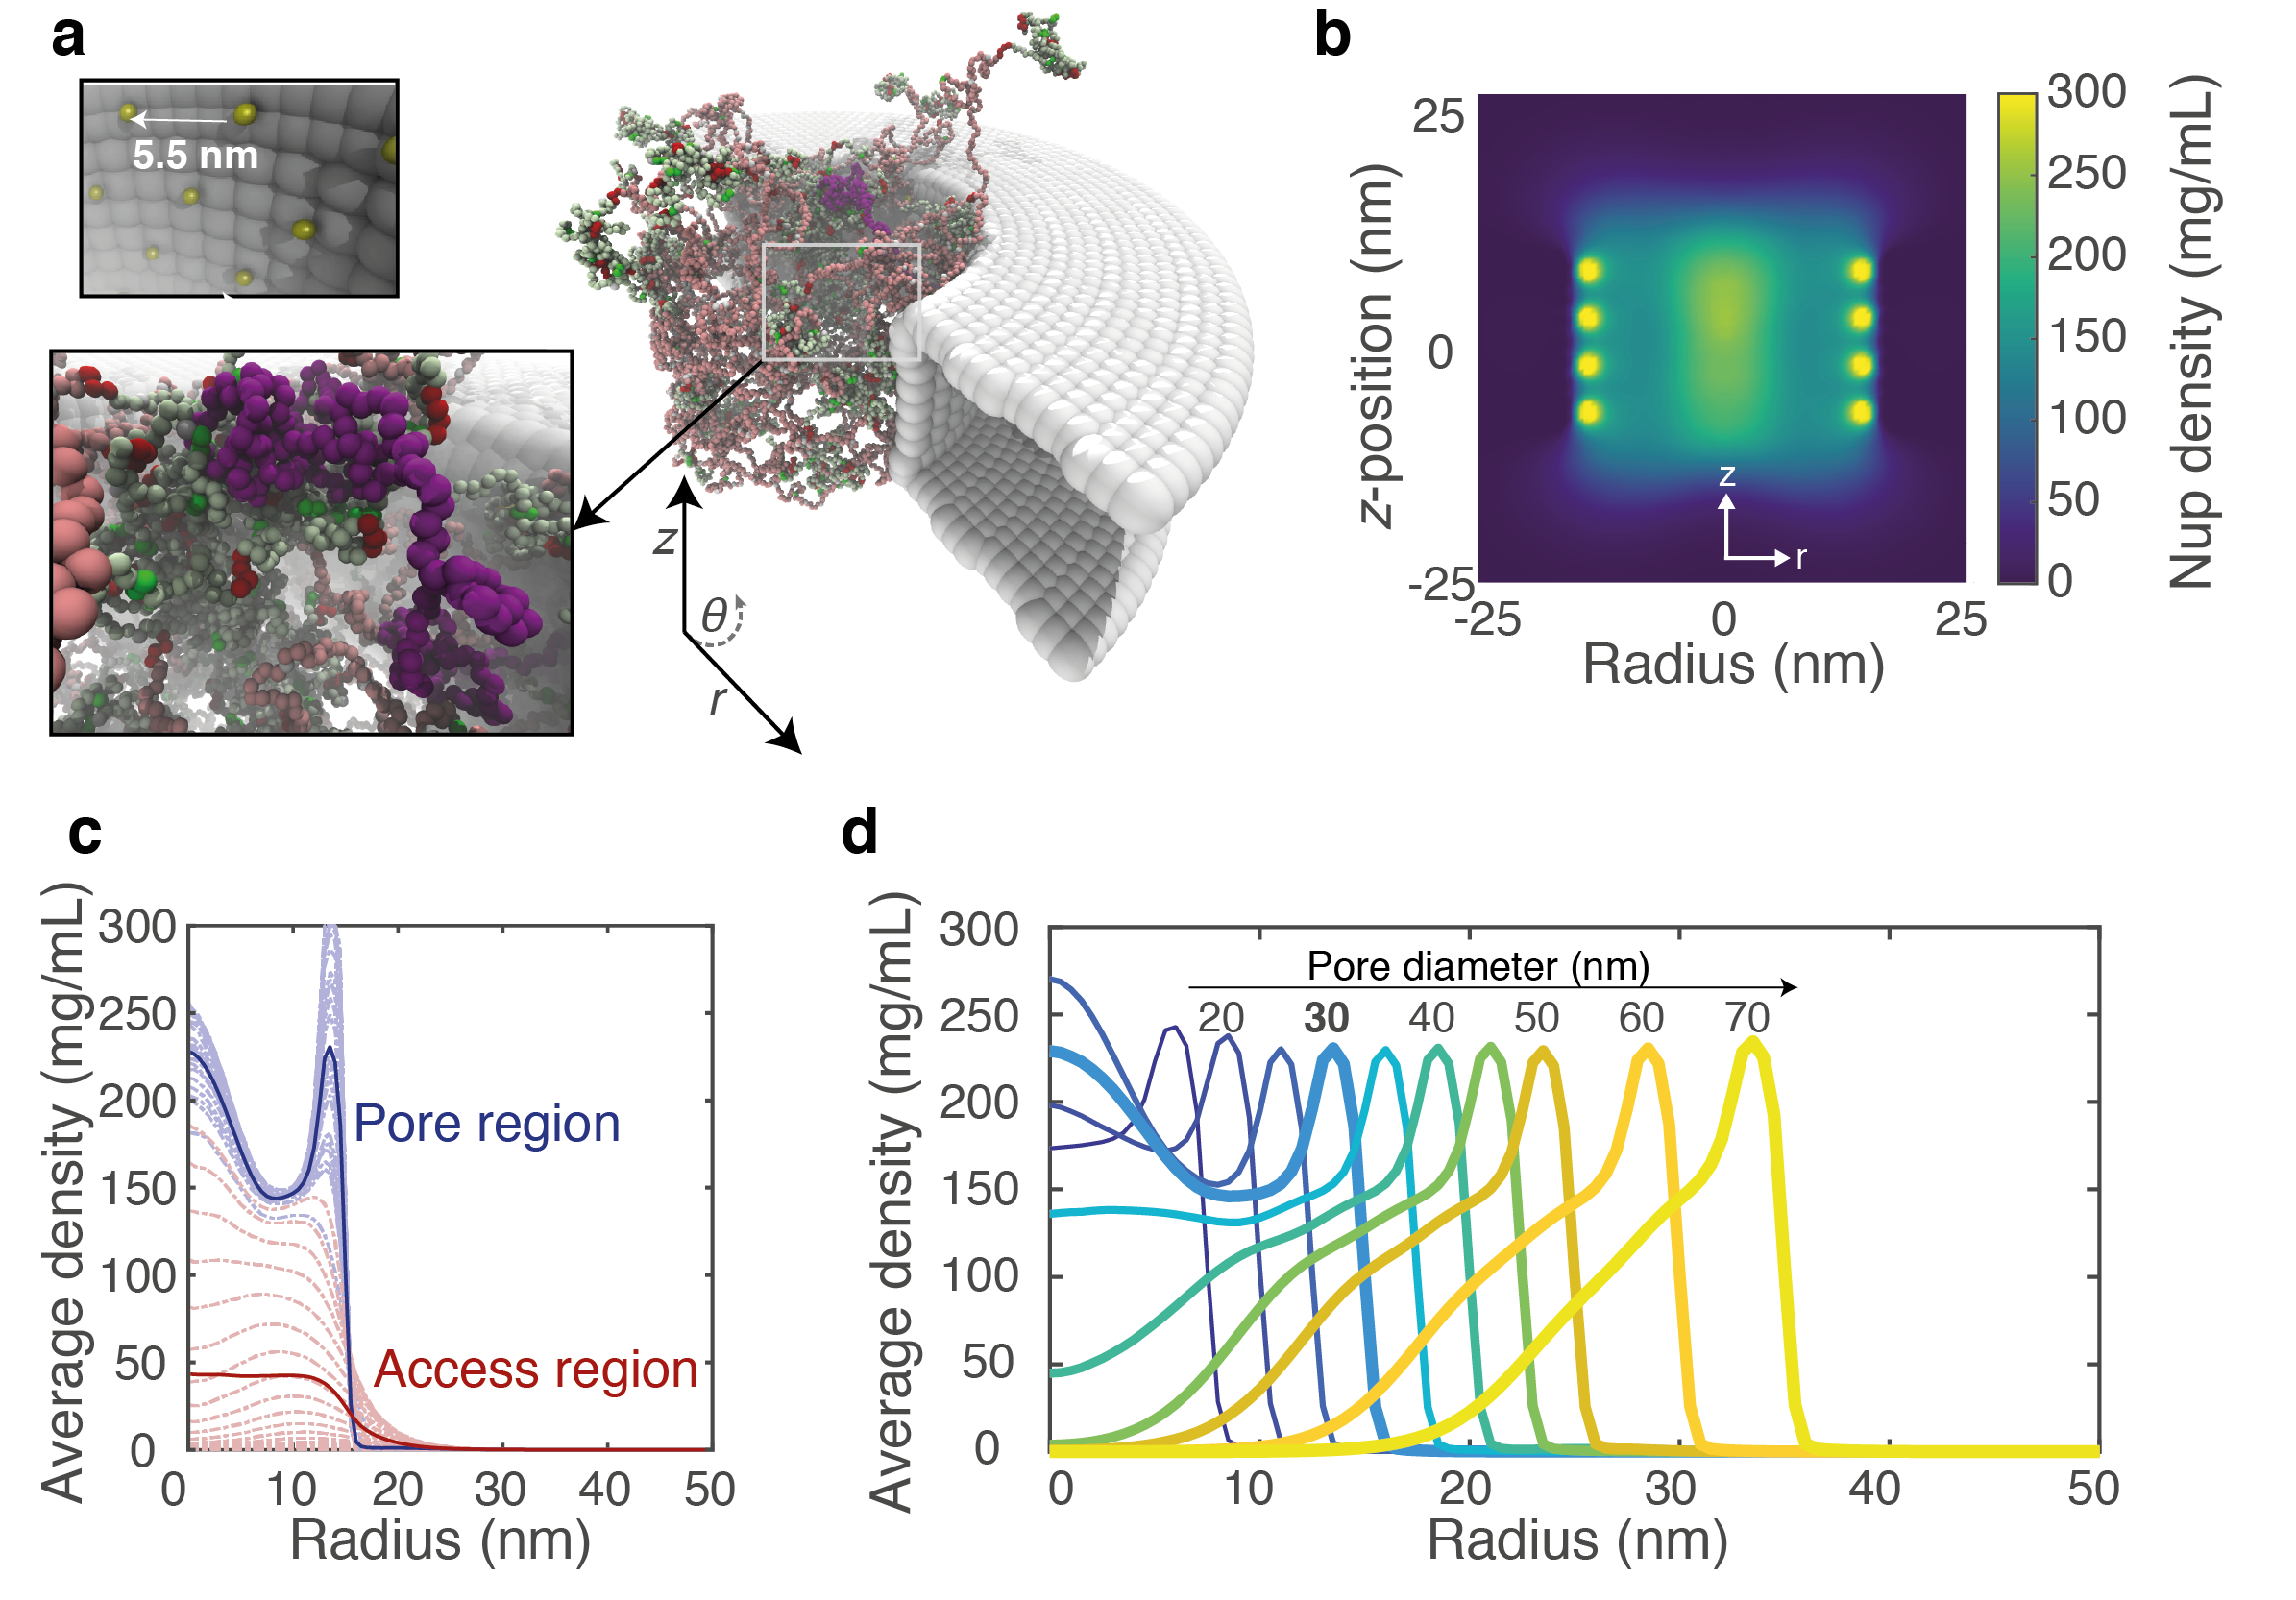
\includegraphics[width=1\linewidth]{figures/Figure4.4.1.png}
	\caption{Protein distribution and conductance of NupX-coated pores.
a, Snapshot of a biomimetic nanopore simulation. NupX proteins (following the colouring scheme of Figure \ref{fig:fig.4.1.1}) were tethered with a grafting distance of 5.5 nm (yellow, top inset) to a cylindrical occlusion made of inert beads (grey). Pore diameters ranged from 15-70 nm, where the pore thickness was 20 nm throughout. Bottom inset: highlight of a single NupX-protein (purple) within the NupX-meshwork. b, Axi-radial map (averaged over time and in the azimuthal direction) of the protein density within a 30 nm NupX-lined nanopore, from 6 $\mu$s simulations. Dark colours indicate regions of low density, brighter colours indicate regions of high density. The collapsed domains of the NupX proteins form a high-density central plug. The high-density regions near the pore radius (15 nm) coincide with the anchoring sites of the NupX proteins. c, Density distributions (thick lines) for the pore (blue, $|z|<$ 10 nm) and access (red, 10 nm $< |z| <$ 40 nm) regions. Dashed curves indicate the average density within 1 nm thick slices in the $z$-direction. d, Radial density distributions ($z$-averaged) for NupX-lined nanopores with diameters ranging from 15 to 70 nm (darker and lighter colours denote smaller and larger diameters, resp.). The curve for 30 nm is emphasized. An increase in pore size beyond 30 nm leads to a decrease in the pore density along the pore’s central channel.}
	\label{fig:fig.4.4.1}	
\end{figure}

\begin{figure}[!htb]
	\centering
	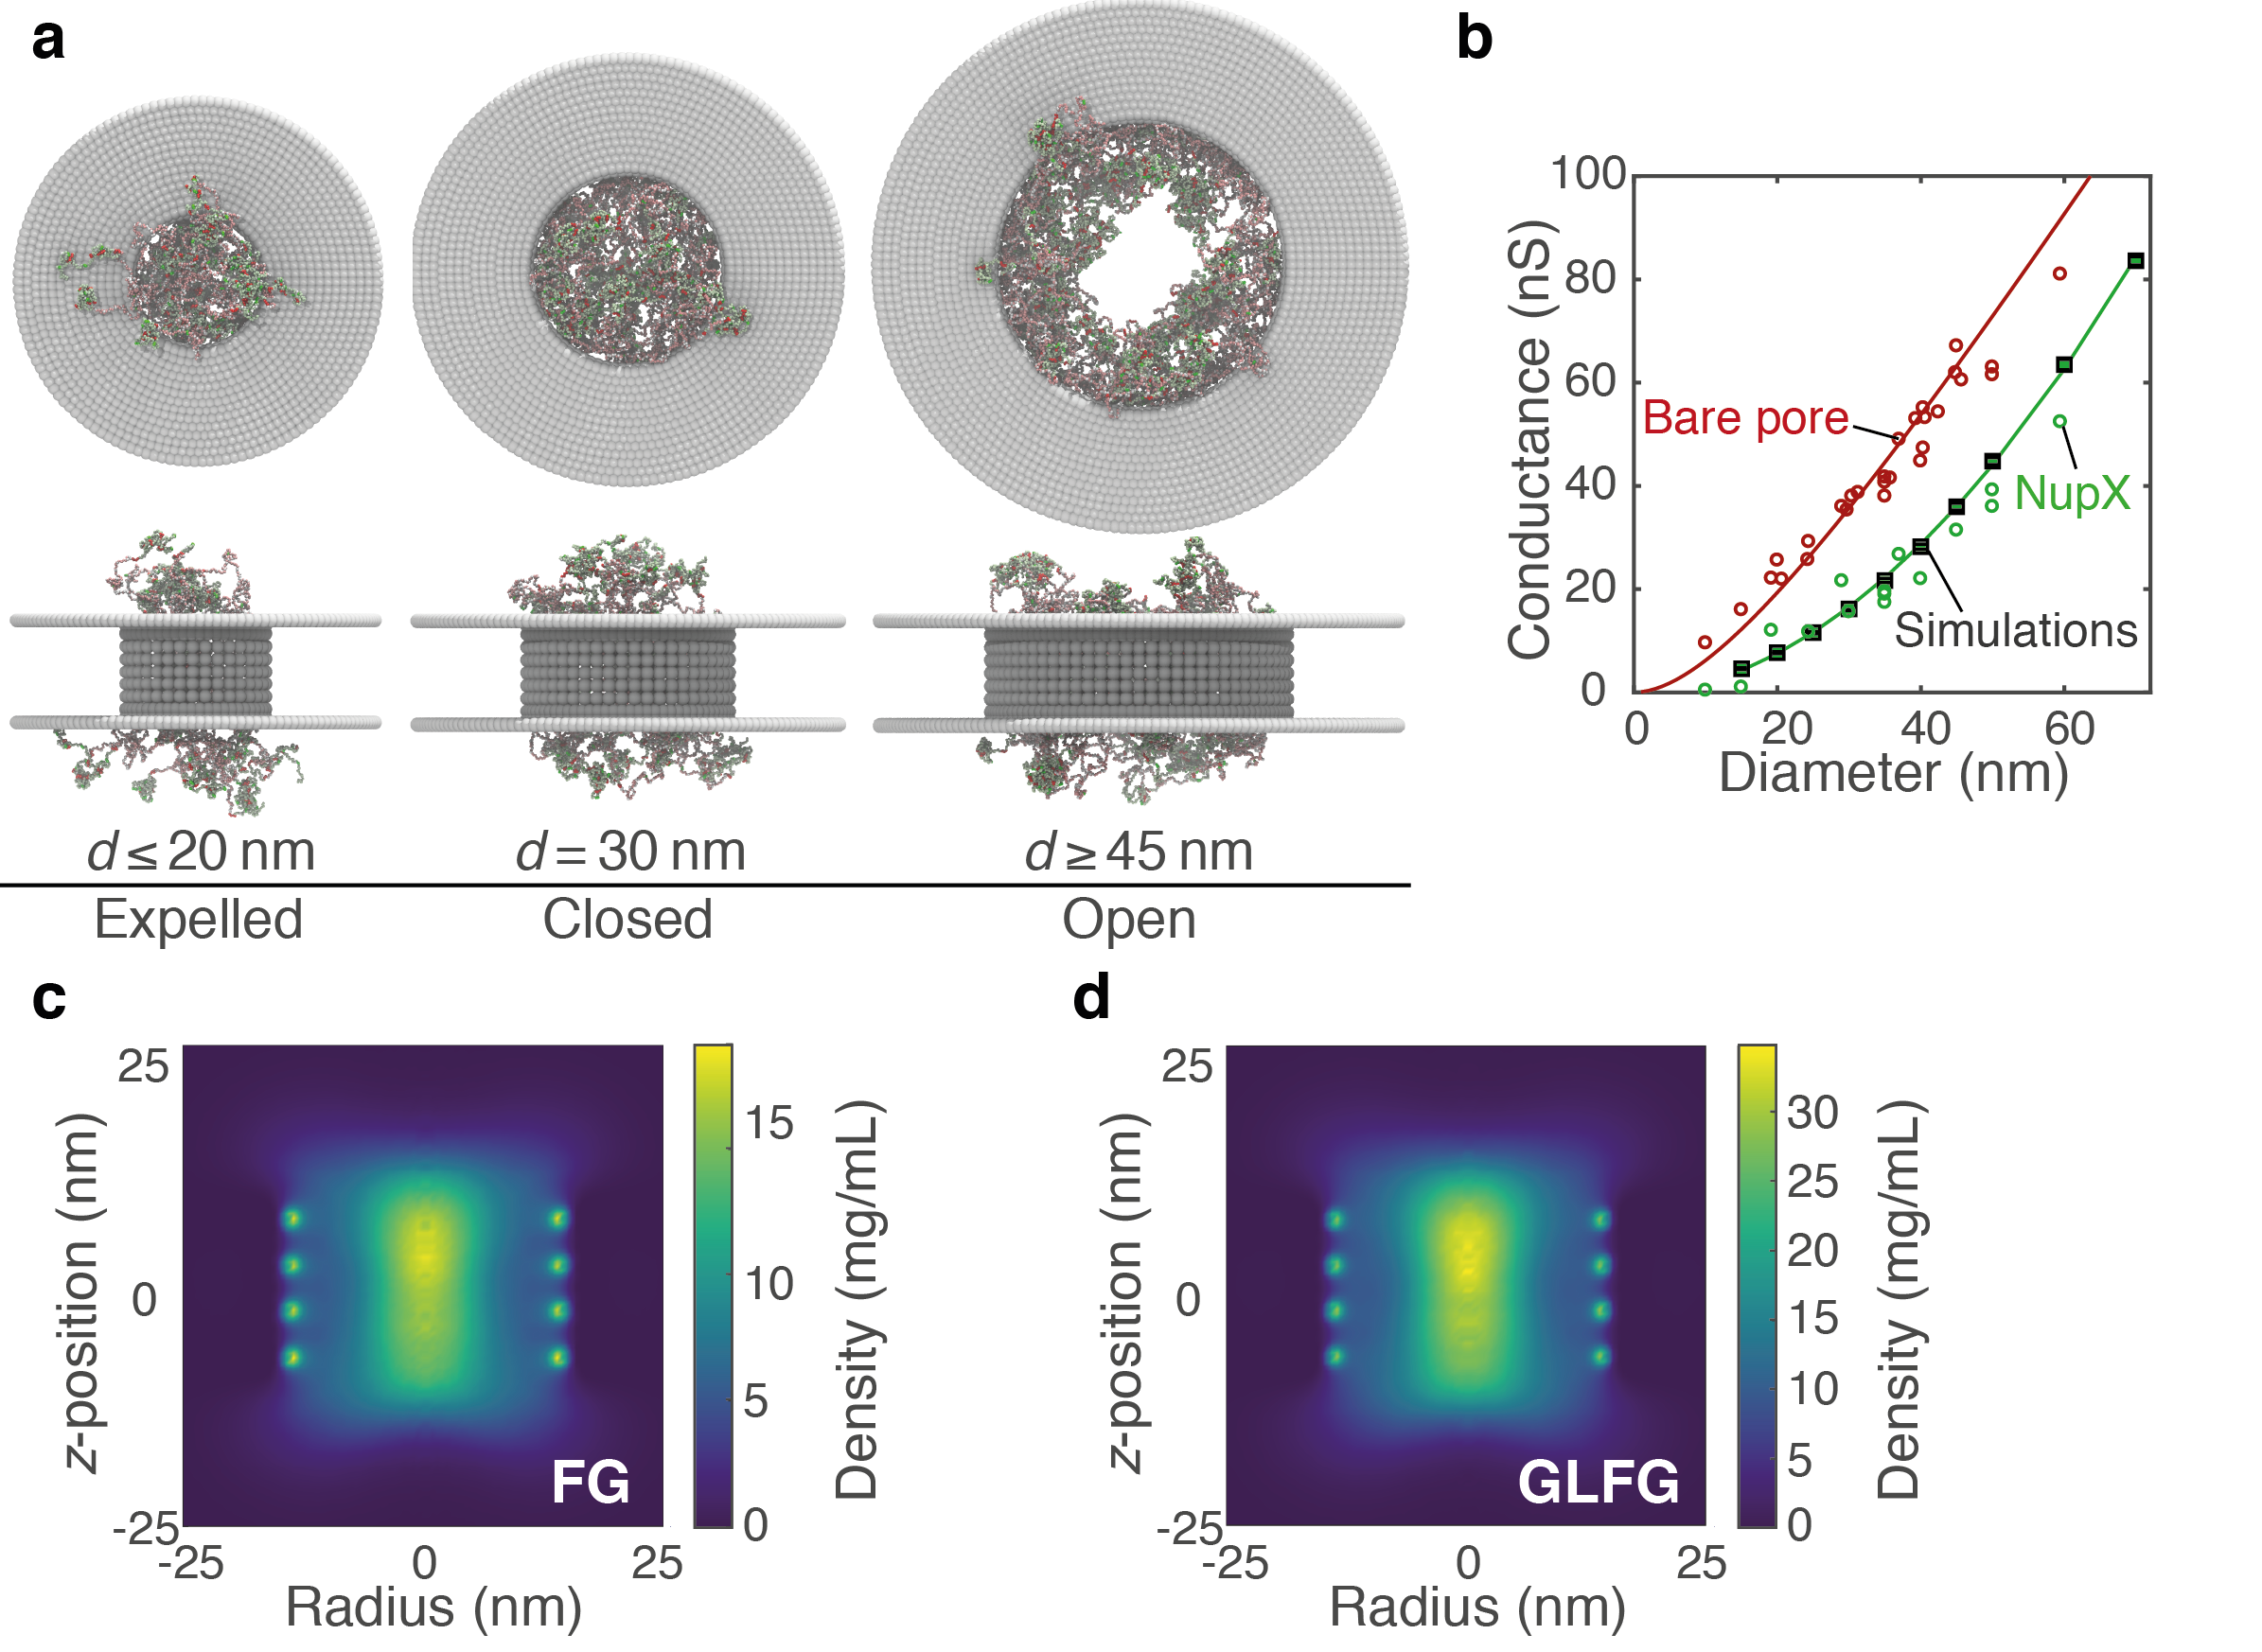
\includegraphics[width=1\linewidth]{figures/Figure4.4.2.png}
	\caption{a, Side-view and top-view visualizations of 20 nm, 30 nm, and 45 nm diameter NupX-lined nanopores. For nanopores with diameters smaller than 25 nm, the pore region density decreases due to an expulsion of the collapsed NupX domains towards the access region. For nanopore diameters larger than 40 nm, the pore density decreases and a hole forms. For nanopore diameters of 25-30 nm, the pore region is sealed by the NupX cohesive domains. b, Conductance scaling for bare and NupX-coated nanopores. Open circles indicate conductance measurements for bare (red) and NupX-coated (green) pores. Squares indicate time-averaged conductance values obtained from MD simulations via a density-conductance relation (Materials and Methods). Error bars indicate the standard deviation in the conductance and are smaller than the marker. Second-order polynomial fits to the bare pore (experimental) and the simulated conductance values are included as a guide to the eye. c,d, Axi-radial density maps for FG and GLFG motifs, respectively. Both types of motif localize in the dense central region, indicating that there is no spatial segregation of different types of FG-motifs in NupX-coated nanopores.}
	\label{fig:fig.4.4.2}	
\end{figure}

High-density regions form close to the attachment sites (\emph{i.e.} the four dots at each wall in Figure \ref{fig:fig.4.4.1}b) and along the central axis of the nanopore. Since the triangulated lattice (comprising four rows) does not strictly exhibit a symmetry plane along the $z=0$ axis, a slight asymmetry ($<10\%$ in terms of protein density) occurs between the top and bottom of the density map. From these data, we obtained a radial protein density profile, averaged over the pore height for the pore region ($|z|< 10$ nm, Figure \ref{fig:fig.4.4.1}c), which exhibits a maximum of 230 mg/mL at the pore center for the 30 nm NupX nanopore system and is insensitive to the aforementioned small asymmetry. This density agrees well with values in the range of 200-300 mg/mL observed in earlier computational studies of the yeast NPC central channel \cite{Huang2020,Ghavami2014}. We attribute the central localization of the NupX proteins to the combination of repulsion between the high C/H ratio extended domains near the pore wall and attraction between the cohesive, low C/H ratio collapsed domains of opposing NupX proteins.  Since the average density in the access region (10 nm $<|z|<$ 40 nm, Figure \ref{fig:fig.4.4.1}c) is found to be low in comparison to the average density within the pore region, we conclude that the NupX proteins predominantly localize within the nanopore. When the grafting distance is perturbed by $\sim10\%$ in either direction (Figure \ref{fig:fig.4.24}) to values of 5.0 or 6.0 nm, similar density profiles are obtained. So even though the experimental grafting distance might be somewhat larger for the nanopore compared to the planar brushes due to the different geometrical confinement, similar profiles would be expected for more sparsely coated pores. 


The organization of the NupX proteins inside the nanopore geometry changes notably with pore diameter (Figures \ref{fig:fig.4.4.1}d,\ref{fig:fig.4.4.2}a). For large diameter pores, the density profile of NupX proteins protruding from the pore surface quite well resembles that of a planar brush (cf. Figure \ref{fig:fig.4.18}), resulting in a central opening for pores that are $>45$ nm. When the pore diameter reaches values $<45$ nm, NupX-coated nanopores are effectively sealed. This 45 nm length scale is remarkable, given the quickly decaying density profile of a planar NupX brush with a similar grafting distance (Figure \ref{fig:fig.4.18}). Upon further decreasing the pore diameter to values $<25$ nm, we find that the NupX collapsed domains are being expelled from the pore region towards the access region, resulting in decreased densities in the central pore region (Figures \ref{fig:fig.4.4.1}d,\ref{fig:fig.4.4.2}a). Interestingly, we find that these changes in NupX morphology as a function of pore diameter are in good qualitative agreement with predictions from earlier works on polymer-coated nanopores \cite{Dimitrov2006,Peleg2011}, which point to a curvature-dependent modulation of the brush height. More specifically, an increase in curvature (\emph{i.e.}, a decrease in pore diameter) of a concave brush substrate is expected to lead to a relative extension of the brush as compared to the planar geometry. Additionally, attractive interactions between the cohesive head groups of NupX anchored at opposing pore walls will also contribute to the sealing of NupX pores. Finally, we note that a central opening in the NupX nanopore meshwork, present for diameters from 45 nm upwards, is consistent with the increased event frequency and translocation speed observed in large (60 nm) NupX-coated pores (Figure \ref{fig:fig.4.22}). 


Using a relation between the local protein density and the local conductivity separately for the pore and access regions \cite{Ananth2018}, we calculated the conductance of the NupX nanopores for varying diameters (Figure \ref{fig:fig.4.4.1}d, Figure \ref{fig:fig.4.25}, Materials and Methods). The calculated conductance from the simulated NupX-lined pores is shown in Figure \ref{fig:fig.4.4.2}b (black squares) together with the experimental conductances for bare and NupX-coated pores (open circles). Note that we adopted a critical protein density of 85 mg/ml from the earlier work on Nsp1 \cite{Ananth2018} in our density-conductivity relation, but assume a different dependency of the local conductivity on the local protein density (Materials and Methods). Rather than assuming an abrupt complete blockage of conductance above the critical protein density of 85 mg/mL, we now use an exponential relation that provides a more gradual reduction in conductance with density. The necessity of a different density-conductance relationship indicates that the conductivity of the NupX nanopore meshwork depends non-linearly on the average protein density. Interestingly, the slope of the conductance-diameter curve for NupX-lined pores converges to that of bare pores already at relatively small pore sizes. This is due to the formation of a hole within the NupX meshwork (Figure \ref{fig:fig.4.4.1}d) already in pores with diameters over 40 nm, rendering these effectively similar to bare nanopores of smaller diameter.


A spatial segregation of different types of FG-motifs, as was observed in recent computational studies \cite{Kim2018,Huang2020}, is not studied here explicitly. However, we find both types of FG-motifs localize similarly in the high-density central region within the NupX nanopore channel (Figures \ref{fig:fig.4.4.2}c,d). From these distributions and the observed selective transport of these pores (Figures \ref{fig:fig.4.3}e-g), we can infer that a spatial segregation of different FG-motifs is not required for selective transport. 


Finally, in order to assess the selective properties of NupX-lined nanopores, we simulated a 30 nm diameter NupX-lined nanopore in the presence of 10 Kap95 or 10 inert particles. We released Kap95/inert particles in the access region at the top and recorded their location in over 5 $\mu$s of simulation time (see Materials and Methods, Figures \ref{fig:fig.4.5}c,d). The Kap95 particles entered and left the NupX meshwork and sampled the pore lumen by traversing in the $z$-direction (Figure \ref{fig:fig.4.5}c). They localized preferentially at positions radially halfway between the central pore axis and the edge of the nanopore, where their time-averaged density distribution takes the shape of a concave cylindrical region, as is shown in Figure \ref{fig:fig.4.5}a. Kap95 was found to be capable of (re-)entering and leaving the meshwork on either side (Figure \ref{fig:fig.4.5}c). Since no external electric field was applied, exiting and subsequent re-absorption of Kap95 into the NupX meshwork occurred and there was no directional preference for the motion of the Kap95 molecules, in contrast to the experiments. 


\begin{figure}[!htb]
	\centering
	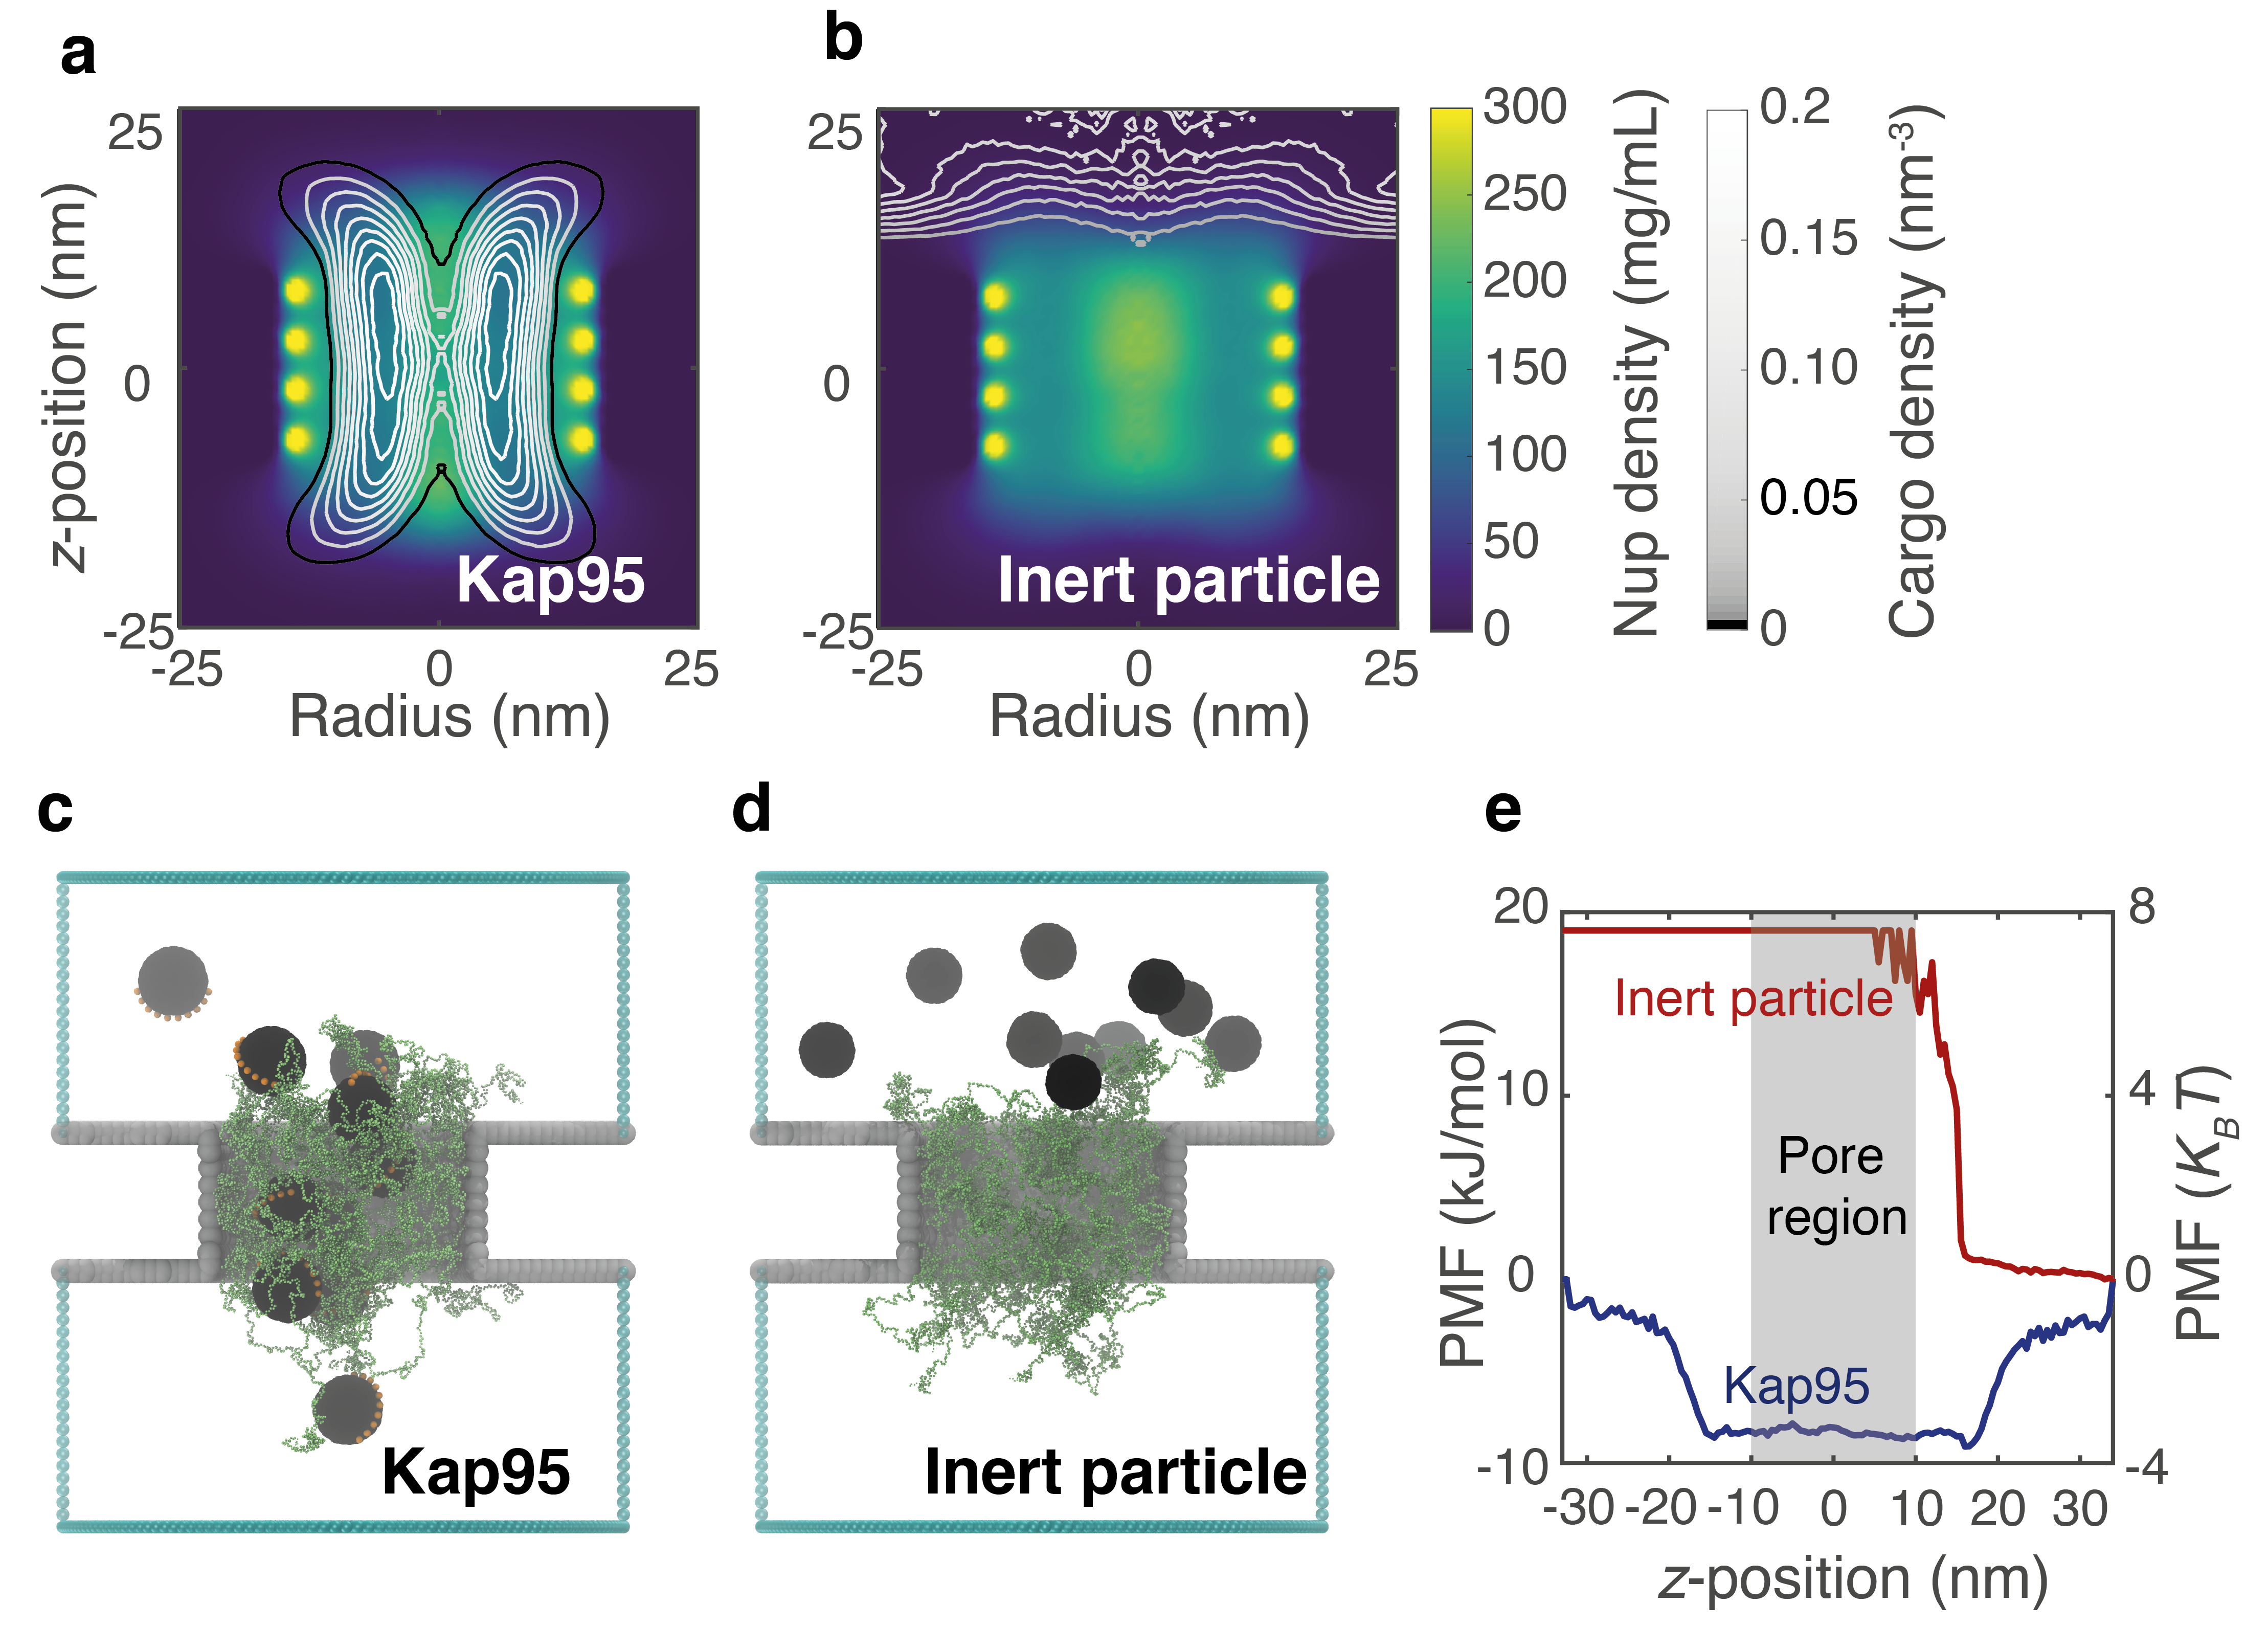
\includegraphics[width=1\linewidth]{figures/Figure4.5.png}
	\caption{Effect of transporters on NupX-lined biomimetic pores. a, Contour graphs of the Kap95 number density (grey contours) superimposed on the NupX protein density distributions (in presence of Kap95) within a 30 nm NupX-lined nanopore (NupX-density follows the same colouring scheme as in Figure \ref{fig:fig.4.4.1}b and is shown separately in Figure \ref{fig:fig.4.26}). The protein meshwork adapts (as compared to the distribution in Figure \ref{fig:fig.4.4.1}b) to accommodate the permeating Kap95 particles. b, Density distribution of inert particles superimposed on the NupX protein density distribution in a 30 nm diameter NupX-lined nanopore. Inert particles remain in the top compartment and do not permeate the NupX-protein meshwork. c, d, Simulation snapshots of 30 nm NupX-lined nanopores in the presence of Kap95 particles (c, black spheres with orange binding spots) and inert particles (d, black spheres), which were released in the top compartment. Kap95 particles enter and exit the NupX meshworks at either side of the nanopore, whereas inert particles remain in the top compartment. e, PMF curves of Kap95 (blue) and inert particles (red) along the $z$-coordinate, obtained via Boltzmann inversion of the normalized density profile along the $z$-axis. The pore region coincides with an energy well of over 3 k\textsubscript{B}T for Kap95, whereas inert particles experience a steep energy barrier of $\sim$7 k\textsubscript{B}T.}
	\label{fig:fig.4.5}	
\end{figure}

\noindent Interestingly, the NupX-meshwork adapted itself to the presence of the Kap95 particles by expanding towards the access region (compare Figures \ref{fig:fig.4.4.1}b and Figure \ref{fig:fig.4.26}): the protein density in the pore region decreased due to the presence of the Kap95, whereas the protein density increased in the access region. In contrast to the findings for Kap95, we observed that the inert particles, simulated under the same conditions, remained in the top compartment (Figure \ref{fig:fig.4.5}b,d) and did not permeate into the NupX-meshwork over the 5 $\mu$s time span of the simulation. 


To quantify the selectivity of the 30 nm NupX-lined nanopores, we calculated PMF-curves along the $z$-axis for both cargo types (Figure \ref{fig:fig.4.5}e, see Materials and Methods). Kap95 experienced a negative free energy difference of approximately 8 kJ/mol, which amounts to a binding energy of just over 3 k\textsubscript{B}T per Kap95. On the other hand, inert particles experience a steep energy barrier of approximately 18 kJ/mol, which corresponds to over 7k\textsubscript{B}T per protein. The obtained Kap95 free energy profiles are similar to those found in other simulation studies of cargo permeation through NPCs \cite{Ghavami2016,Tagliazucchi2013} or NPC mimicking systems \cite{Ananth2018,Ro2018}. The Kap95 binding free energy differences along the nanopore axis are considerably smaller than the computed free energy profiles for NupX-brushes (Figure \ref{fig:fig.4.2}i). This most probably relates to the fact that the two studied reaction coordinates differ notably and cannot easily be compared: the reaction coordinate in Figure \ref{fig:fig.4.2}i describes orthogonal entry into a brush that extends infinitely in the lateral direction, whereas the coordinate in Figure \ref{fig:fig.4.5}e describes lateral entry and exit into the NupX assembly within the pore. As a result, one would not expect the free energy differences for transport through the nanopores to be similar to those obtained for entry into a brush geometry. Note that large free energy differences in our nanopores would also yield residence times that are orders of magnitude larger than the observed $\sim$ms dwell times in our nanopore experiments\cite{Tetenbaum-Novatt2012} (Figure \ref{fig:fig.4.3}f). From our combined experimental and simulation results, we conclude that NupX-lined nanopores indeed reproduce the NPC’s remarkable selectivity towards Kap95. 


\section{Conclusion}

In this work, we introduced a 311-residue long artificial FG-Nup, termed NupX, that we rationally designed \emph{de novo} based on the average properties of GLFG-type Nups (Nup49, Nup57, Nup100, Nup116, Nup145N) and which faithfully mimics the selective behaviour of the nuclear pore complex. We experimentally found that substrates coated with NupX brushes of varying grafting densities bind selectively to Kap95, while they did not interact with the control BSA proteins – a finding confirmed through coarse-grained MD simulations of the adsorption of Kap95 and inert particles. Consistent with these results, we found that Kap95 translocates through both uncoated and NupX-lined nanopores on a physiological ($\sim$ms) timescale \cite{Ribbeck2001}, whereas BSA passage through the NupX-coated pores was effectively excluded. Coarse-grained MD simulations revealed how the NupX proteins form a dense ($>150$ mg/mL) phase that allows passage of Kap95 particles while excluding inert particles. Interestingly, we find that the high densities of the FG-rich NupX meshworks are comparable to those obtained in earlier simulation studies of yeast NPCs \cite{Ghavami2014}. A comparison of the intrinsic protein density (\emph{i.e.} the protein density of an individual molecule in solution, quantified by the mass per unit Stokes volume) of NupX (219 mg/mL) with that of Nsp1 (74 mg/mL) explains why our NupX-meshworks have the tendency to localize more compactly inside nanopore channels than Nsp1 in earlier work \cite{Ananth2018}. The increased conductance of the denser NupX-lined nanopores (as compared to Nsp1) required a non-linear relation between the average protein density and the local conductivity, and indicates that the average protein density is not the only factor that describes conductivity; the dynamics of the unfolded proteins and the local charge distribution might be important as well. 


The design strategy presented in this work allows us to assess the role of the amino acid sequence of the spacer regions in GLFG-Nups. Spacer residues were reported to be involved in the interaction interface of Nup-NTR complexes \cite{Milles2015,Liu2005,Raveh2016}, highlighting a possible specific role of these domains in the binding of NTRs. In the current work, we assigned the positions of spacer residues along the NupX amino acid sequence entirely randomly, in both the collapsed, FG-rich low C/H ratio domain, and the extended high C/H ratio domain. This indicates that no specific spacer sequence motifs are required to facilitate the fast and selective transport of NTRs like Kap95. The consistency of the Stokes’ radii of different NupX designs within our simulations (Figure \ref{fig:fig.4.1.2}f) supports this finding. 


Furthermore, our results shed light on the functional role of the spatial segregation of FG and GLFG motifs that was observed in earlier work \cite{Kim2018,Huang2020}. Although these recent computational studies observed such a feature and suggested that it plays a role in selective transport, the coinciding distributions of FG and GLFG motifs (Figures \ref{fig:fig.4.4.2}c,d) show that no spatial segregation of different types of FG motifs exists within our selective nanopores. Notably, this does not rule out a different functional role for the spatial segregation of different types of FG-motifs, which can be explored in future work.


The combined design and characterization approach presented here, with brush-adsorption and nanopore-transport measurements on the one hand and coarse-grained MD simulations on the other, provides a powerful and exciting platform for future studies of artificial FG-Nups: one can now start to systematically examine the relation between FG-Nup amino acid sequence and size selectivity of the NPC. Such studies could, for example, entail the design of FG-Nups with radically different physicochemical properties (\emph{i.e.} FG-spacing, FG motif type, spacer domain C/H ratios, sequence complexity) to assess the selective properties of nanopore systems functionalized with these designer FG-Nups.  Indeed, solid-state nanopores modified with a single type of FG-Nup were shown in this and other works \cite{Jovanovic-Talisman2009,Kowalczyk2011a,Ananth2018} to reproduce NPC selectivity, justifying the use of a single type of artificial Nups within an environment structurally similar to the NPC. Moreover, in view of the similarity \cite{Yamada2010} and redundancy \cite{Adams2016,Strawn2004} of different FG-Nups within the NPC and the ability of our method to robustly reproduce FG-Nup properties (Figure \ref{fig:fig.4.1.2}f and Figure \ref{fig:fig.4.27}), we are confident that a single artificial FG-Nup can capture the selective barrier function the NPC. However, given that even minimally viable native NPCs \cite{Adams2016,Strawn2004} contain several different FG-Nups, it is worth mentioning that NPC mimics with a heterogeneous set of (artificial) FG-Nups can be created as well: DNA origami scaffolds \cite{Ketterer2018} potentially allow to position different artificial FG-Nups with great control, thus enabling systematic studies of how the interplay of different (artificial) FG-Nups gives rise to various transport properties of the NPC. 


Finally, the design procedure that we introduced here is not limited to applications in nucleocytoplasmic transport. It may, for example, be possible to use a comparable approach to create \emph{de novo} selective molecular filters (\emph{e.g.} for use in artificial cells \cite{Buddingh2017,Spoelstra2018}), systems that would rely on selective partitioning of molecules in meshworks of unfolded proteins with assigned properties. Control can be asserted over the composition and geometry of the meshwork \emph{e.g.} by means of recently developed DNA-origami scaffolds \cite{Fisher2018,Ketterer2018}. More generally, the approach illustrated here may enable future studies of the physical properties underlying phase separation of intrinsically disordered proteins\cite{Schmidt2015}. One could, for example include degrees of freedom such as the proteins’ second virial coefficient ($B_{22}$), or the charge patterning ($\kappa$), which have been linked to the phase behavior of intrinsically disordered proteins \cite{Das2013,Dignon2018}. We envision that just like the field of de novo protein design has come to fruition with improved understanding of protein folding \cite{Huang2016}, the design of unstructured proteins like NupX will enable a versatile platform to study the intriguing functionality of intrinsically disordered proteins.


\section{Methods}

\subsection{Analysis of GLFG-Nups and design of synthetic Nups}

Protein sequences of \emph{Saccharomyces cerevisiae} GLFG-type Nups (\emph{i.e.} Nup100, Nup116, Nup49, Nup57 and Nup145N) were analyzed using a script custom-written with $R$ programming package (version 3.3.1). Following the definitions of high C/H-ratio and low C/H-ratio unfolded FG-Nup domains as given in Ref. \cite{Yamada2010}, we obtained histograms of the amino acid frequencies in both the collapsed (low C/H-ratio) and extended (high C/H-ratio) domains. The collapsed / extended domain sequences of NupX were then assigned in three steps: First, the collapsed and extended domains of NupX were assigned equal lengths of 150 residues each. Then, by normalizing the distributions in Figure \ref{fig:fig.4.1.2}b to the number of available residues within each domain, the total pool of amino acids within each domain was obtained. Lastly, these amino acids were randomly assigned a sequence index within each domain, with a boundary condition of the presence of FG and GLFG repeats spaced by 10 residues within the low C/H-ratio domain. This approach was repeated iteratively in combination with disorder predictions using the on-line PONDR disorder prediction utility \cite{Peng2006} until a sufficiently disordered design was obtained. The final version of the NupX amino acid sequence was also analyzed for secondary structure using DISOPRED \cite{Jones2015a,Ward2004} and Phyre2 \cite{Kelley2015}. A 6-histidine tag was added to the N-terminus of the NupX sequence in order to facilitate protein purification (see Protein purification section). Finally, on the C-terminus a cysteine was included to allow the covalent coupling of the NupX protein to the surface.


\subsection{Expression and purification of NupX and Kap95}

The synthetic NupX gene (Genscript), appended with codons for an N-terminal His6-tag and a C-terminal cysteine residue, was cloned into pET28a and expressed in \emph{Escherichia coli} ER2566 cells (New England Biolabs, \emph{fhuA2 lacZ}::T7 gene1 [\emph{lon}] \emph{ompT gal sulA11} R(mcr73::miniTn10--TetS )2 [\emph{dcm}] R(zgb-210::Tn10--TetS ) \emph{endA1} $\Delta$(mcrCmrr)114::IS10). To minimize proteolysis of NupX, the cells were co-transformed with plasmid pED4, a pGEX-derivative encoding GST-3C-Kap95 under control of the tac promoter. Kap95 was expressed as a C-terminal GST fusion protein in \emph{Escherichia coli} ER2566 cells from plasmid pED4, a pGEX derived construct in which the thrombin cleavage site
was replaced by a 3C protease cleavage site using primers ed7 and ed8 (Table \ref{tab:table4.4}). Cells were cultured in shake flasks at $37^{\circ}$C in Terrific Broth supplemented with 100 $\mu$g/mL ampicillin and 50 $\mu$g/mL kanamycin, and expression was induced at OD600$\sim$0.6 with 1 mM IPTG. After 3 hours of expression the cells were harvested by centrifugation, washed with PBS, resuspended in buffer A1 (50 mM Tris/HCl pH 7.5, 300 mM NaCl, 8 M urea, 5 mg/mL 6-aminohexanoic acid supplemented with one tablet per 50 mL of EDTA-free cOmplete ULTRA protease inhibitor cocktail) and frozen as “nuggets” in liquid nitrogen. Cells were lysed with a SPEX cryogenic grinder, after thawing 1,6-hexanediol was added to a final percentage of 5\%, and the lysate was centrifuged for 30 minutes at 125000 xg in a Ti45 rotor (Beckman Coulter). The supernatant was loaded onto a 5 mL Talon column mounted in an Akta Pure system, the column was washed with buffer A2 (50 mM Tris/HCl pH 7.5, 300 mM NaCl, 800 mM urea, 5 mg/mL 6-aminohexanoic acid, 2.5\% 1,6-hexanediol) and NupX was eluted with a linear gradient of 0-200 mM imidazole. Peak fractions were pooled, diluted tenfold with buffer A2 lacking sodium chloride, loaded onto a 1 mL HiTrap SP sepharose HP column and NupX was eluted with a linear gradient of 0-1 M NaCl.


Kap95 was expressed as a C-terminal GST fusion protein in \emph{Escherichia coli} ER2566 cells from plasmid pED4, a pGEX derived construct (kindly provided by Jaclyn Novatt) in which the thrombin cleavage site was replaced by a 3C protease cleavage site. Cells were grown in shake flasks at $30^{\circ}$C on LB medium supplemented with 100 $\mu$g/mL ampicillin, induction was induced at OD600$\sim$0.6 with 1 mM IPTG, and growth was continued overnight. Cells were harvested by centrifugation, washed with PBS, resuspended in TBT buffer (20 mM HEPES/NaOH pH 7.5, 110 mM KOAc, 2 mM MgCl\textsubscript{2}, 0.1\% (w/v) Tween20, 10 $\mu$M CaCl\textsubscript{2} and 1 mM $\beta$-mercaptoethanol), and lysed by a cell disruptor (Constant Systems) at 20 kpsi. Following centrifugation for 30 minutes at 125000 xg in a Ti45 rotor (Beckman Coulter), the supernatant was loaded onto a 2 mL GSTrap 4B column mounted in an Akta Pure system. The column was washed with TBT buffer, TBT + 1 M NaCl and TBT + 0.1 mM ATP, and the fusion protein was eluted with TBT + 10 mM reduced glutathione. The GST moiety was cleaved off by overnight digestion with home-made 3C protease, and Kap95 was separated from GST and the protease by size exclusion chromatography on a Superdex S200 column pre-equilibrated with TBT buffer.


\subsection{QCM-D sample preparation and data acquisition}
QSense Analyzer gold- and SiN-coated quartz QCM-D chips were purchased from Biolin Scientific, Västra Frölunda, Sweden. Prior to the experiment, chips were immersed in RCA-1 solution, which consisted of 30\% Ammonium Hydroxide, 30\% Hydrogen Peroxide, and deionized (DI) water in 1:1:5 ratio, for $\sim$30 minutes at $75^{\circ}$C. This step was used to clean the surface from carbon species, as well as to enrich the surface with hydroxyl groups in case of the SiN-coated chips. Chips were further rinsed with DI water, sonicated for $\sim$10 minutes in pure ethanol, and blow-dried with a nitrogen stream. Before each experiment, flow-cells were disassembled, cleaned by sonication for 20-30 minutes in freshly prepared 2\% SDS, rinsed with DI water, and blow-dried with a nitrogen stream. For SiN-coated quartz sensors, the SiN surface was chemically engineered in order to add free maleimide groups (see Preparation of NupX-coated nanopores for details). Prior to the coating of the gold surface, protein solutions containing either NupX, Nsp1, or Nsp1-S, were incubated in PBS with 1mM TCEP for at least half an hour, which was also present during the coating step. Similarly, MUTEG solutions included also 10mM TCEP.
QMC-D data were monitored and recorded with sub-second resolution using Qsoft, which was provided by the company together with Qsense Analyzer. Buffer was injected into the flow-cell chamber at constant flow-rate of 20 $\mu$L/min using a syringe pump. Experiments were all performed at room temperature. Shift in the resonance frequency ($\Delta$f) and dissipation ($\Delta$D) can be, in first approximation, attributed to changes in deposited mass and viscoelastic properties of the film, respectively. $\Delta$f and $\Delta$D were acquired at the fundamental tone (n = 1) and the 5 overtones (n = 3, 5, 7, 9, 11). The normalized second overtone $\frac{\Delta f_5}{5}$ was used for display and analysis. Data processing and plotting were performed using a custom-written Matlab script. 


\subsection{SPR measurements and analysis}
All measurements were performed using a Bionavis MP-SPR Navi\textsuperscript{Tm} 220A instrument equipped with two 670 nm laser diodes focused on two different spots on the sample surface. Both gold and silicon dioxide coated sensor slides were used (Bionavis). Grafting of proteins or MUTEG to the gold and silica coated sensors was performed using the same protocol as for the gold-coated QCM-D chips and for the nanopore chips, respectively. After the final incubation step, the chips were rinsed with milliQ water, ethanol, and gently blow-dried with pure nitrogen. Immediately before measurements of the sensors in air, the backside of each sensor was cleaned by carefully rubbing lint-free lens tissue soaked in 2-propanol (Sigma Aldrich) followed by blow-drying both sides with nitrogen. At least two repeat measurements were performed for all sensor slides to verify no signal drifting occurred due to adsorption of moisture. The background signal from each sensor was measured before grafting the adlayers to the sensor surfaces and was used as a starting point for modelling the adlayer thickness, $d$. The silicon dioxide thin film thickness was evaluated to $15.1\pm0.5$ nm across the different samples and surface spots prior to surface grafting. Three replicate sensor slides were used for each type of adlayer (except for MUTEG which used 1 sensor slide per concentration measurement). 


Adlayer thickness was determined from least-square fitting measurements with Fresnel models using an approach similar to those used in previous works \cite{Emilsson2015,Emilsson2017}, which we briefly describe here. The following information was used to obtain adlayer thickness: a fit performed on the angular reflectivity spectra close to the resonance angle (see Figure \ref{fig:fig.4.10}), knowledge of the sensor layer thicknesses and refractive indices \cite{Ferrand-DrakeDelCastillo2018}, the bulk refractive index of air in the measurement cell, as determined from the total internal reflection angle of each measurement, and the assumption that the adlayer refractive index $n$ is the same as its dry bulk counterpart ($n_{protein} = 1.53$ 73, $n_{APTES} = 1.42$, $n_{MUTEG} = 1.456$ 74). The formed adlayers were further assumed to be homogeneous and not containing solvent and to be free of contaminants. Grafting densities, $\Gamma$, of MUTEG, Nsp1, Nsp1-S and NupX were obtained from the Fresnel model determined $d$ using the relation: 


\begin{equation}\label{eqn:4.1}
\Gamma=\frac{\rho d N_A}{M}
\end{equation}

where $\rho$ is the density ($\rho_{MUTEG} = 1.09$ g/cm\textsuperscript{3}, $\rho_{protein} = 1.35$ g/cm\textsuperscript{3}; Ref. 70), $N_A$ is Avogadro’s constant, and $M$ is the molecular weight ($M_{MUTEG} = 380$ Da, $M_{Nsp1} = 65.7$ kDa, $M_{Nsp1-S} = 62.1$ kDa, $M_{NupX} = 32.5$ kDa).  


\subsection{Preparation of NupX-coated nanopores and current data acquisition}

Solid-state nanopores with diameters from 10-60 nm were drilled using TEM in glass-supported SiN\textsubscript{x} free-standing membranes. Glass chips were purchased from Goeppert. We refer to Ref. \cite{Balan2014,Balan2015} for details on the fabrication of the chip substrate and free-standing membrane. Freshly drilled solid-state nanopores were rinsed with ultrapure water, ethanol, acetone, and isopropanol, followed by 2-5 minutes of oxygen plasma treatment, which was performed in order to further clean and activate the nanopore surface with hydroxyl groups. Next, chips were incubated in 2\% APTES (3-aminopropyl-triethoxysilane) (Sigma Aldrich) in anhydrous toluene (Alfa Aesar) for 45-60 min at room temperature, shaking at 400 rpm, followed by 15 minutes in anhydrous toluene for washing. These two steps were performed in a glove-box under constant nitrogen stream in order to prevent the APTES from polymerizing. Then, chips were further rinsed with ultrapure water, ethanol, and heated at $110^{\circ}$C for at least 30 minutes. This step was used to fixate the APTES layer by favouring further binding between the unreacted ethoxy groups. 


The nanopore surface was thus covered with primary amines, which were subsequently reacted to Sulfo-SMCC (sulphosuccinimidyl-4-(N-maleimidomethyl)-cyclohexane-1-carboxylate) (2 mg no-weight capsules (Pierce)), a crosslinker that contains NHS-ester (reacts to amines) and maleimide (reacts to thiols) groups at opposite ends, for $>3$ hrs at room temperature, shaking at 400 rpm. Chips were subsequently washed in PBS for 15 minutes and incubated with thiolated proteins for 2-3 hours, which were pretreated with 5 mM TCEP for $\sim$30 minutes in order to reduce the thiol groups. Chips were further washed in PBS before the electrical measurement. Raw ionic current traces were recorded at 100 kHz bandwidth with an Axopatch 200B (Molecular devices) amplifier, and digitized (Digidata 1322A DAQ) at 250 kHz. Traces were monitored in real-time using Clampex software (Molecular devices). Data were digitally filtered at 5 kHz using a Gaussian low-pass filter and analysed using a custom-written Matlab script76.


\subsection{Dynamic light scattering (DLS) measurement of the hydrodynamic diameter}

DLS experiments were performed using Zetasizer Nano ZS (Malvern). Cuvette of 100 $\mu$L (Brand GMBH) were used for the measurement. All protein hydrodynamic diameters were measured in 150 mM KCl, 10 mM Tris, 1mM EDTA, at pH 7.5, and averaged over three experiments. Mean value and standard deviation for each of the proteins used are reported in Table \ref{tab:table4.1}. Proteins which contained exposed cysteines (NupX, Nsp1, and Nsp1-S) were pre-treated with TCEP (present in at least 100$\times$ excess) in order to break disulfide bonds. 

\subsection{Coarse-grained model for unfolded proteins}
All coarse-grained MD-simulations were performed using our earlier developed one-bead-per-amino acid (1BPA) model for unfolded proteins \cite{Ghavami2014,Ghavami2013}. This model maps complete amino acids to single beads with a mass of 124 amu placed on the C\textsubscript{$\alpha$} position, separated by an average bond length (modelled as a stiff harmonic potential) with an equilibrium distance of 0.38 nm. Backbone potentials were assigned via an explicit coarse-grained mapping of Ramachandran data of a library of the coil regions of proteins that distinguishes flexible (\emph{i.e}. Glycine), stiff (\emph{i.e.} Proline) and regular amino acids \cite{Ghavami2013}. Non-bonded interactions between different amino acid residues are based on their respective hydrophobicity (normalized between 0 and 1 and based on the free energy of transfer between polar and apolar solvents) and obey the following interaction potential \cite{Ghavami2014}:


\begin{numcases}{\Phi_{HP}=}
 \epsilon_{rep}\left(\frac{\sigma}{r}\right)^8-\epsilon_{ij}\left[\frac{4}{3}\left(\frac{\sigma}{r}\right)^6-\frac{1}{3}\right], & $r\leq \sigma$ \label{eqn:4.2}
\\
(\epsilon_{rep}-\epsilon_{ij})\left(\frac{\sigma}{r}\right)^8, & $\sigma\leq r$ \label{eqn:4.3}
\end{numcases}


\noindent where $\epsilon_{rep}=10$ kJ/mol and $\epsilon_{ij}=13\cdot\sqrt{(\epsilon_{i}\epsilon_{j})^{\alpha}}$ kJ/mol, with $\epsilon_{i}$ the normalized (between 0 and 1) hydrophobicity of a residue $i$ and $\alpha=0.27$ a scaling exponent. The electrostatic interactions within the 1BPA model are described by a modified Coulomb law:

\begin{equation}\label{eqn:4.4}
\Phi_{EL}=\frac{q_iq_j}{4\pi \epsilon_0\epsilon_r(r)r}\exp(\kappa r),
\end{equation}

\noindent where the electrostatic interactions are modulated via a Debye screening component. This form of electrostatics takes into account the salt concentration (set at 150 mM here, via a screening length $\kappa=1.27$ nm\textsuperscript{-1}) together with a solvent polarity at short distances via a distance-dependent dielectric constant:


\begin{equation}\label{eqn:4.5}
\epsilon_r(r)=80\left[1-\frac{r^2}{z^2}\frac{e^{\frac{r}{z}}}{\left(e^{\frac{r}{z}}-1\right)^2}\right],
\end{equation}

\noindent where $z=0.25$. Non-bonded interactions are cut-off at 2.5 nm (hydrophobic interactions) or 5.0 nm (electrostatic interactions). Since the 1BPA model operates without explicit solvent, we apply stochastic dynamics with a coupling frequency $\tau_T$ of 50 ps\textsuperscript{-1}. Stochastic dynamics handles temperature coupling implicitly, ensuring that the system operates within a canonical ensemble at a reference temperature of 300 K. We refer the reader to the original work for further details on the used 1BPA model \cite{Ghavami2014,Ghavami2013}. Unless otherwise mentioned, all simulations were performed using the above forcefield and corresponding settings, employing the GROMACS \cite{VanDerSpoel2005} molecular dynamics software (version 2016.1/2016.3) on a parallelized computer cluster. A complete overview of all simulations in this work is provided in Table \ref{tab:table4.3}.


\subsection{Calculating Stokes radius of NupX and variations}
Intrinsically disordered proteins were modelled using the 1BPA model \cite{Ghavami2014,Ghavami2013}, starting from an extended configuration. After energy minimization (steepest descent) and a brief (5 ns) equilibration step, we simulated the individual proteins for $5\cdot10^8$ steps using a timestep of 20 fs (total simulation time: 10 $\mu$s). Conformations were extracted every 10000 frames (\emph{i.e.}, every 200 ps). In order to calculate the Stokes radii ($R_s$) from the MD trajectories, we extracted protein conformations every 2 ns and applied the HYDRO++ software \cite{Ortega2011} in order to calculate the $R_s$-values. This procedure yields a total of 5000 Stokes radii per protein.


\subsection{Calculating NupX brush density profiles and PMF curves of cargo adsorption}

We modelled the brush substrate as a fully triangulated (sometimes denoted as hexagonally) closed-packed array of sterically inert beads with a diameter of 3 nm. NupX proteins were tethered on top of the scaffold by their C-terminus, following an equilateral triangular lattice with a uniform grafting distance of 4.0 or 5.7 nm. A fully triangulated lattice is close-packed in two dimensions, meaning that a unique length scale sets the grafting density. The simulation box consisted of a $24\times24\times81.5$ nm\textsuperscript{3} triclinic and fully periodic unit cell (Figure \ref{fig:fig.4.2}h). In our simulation of a less dense brush (grafting distance of 5.7 nm), the simulation box size was accordingly scaled up to 34.2 nm in the lateral dimensions. The grafting pattern of the NupX proteins was placed such as to ensure homogeneity of the NupX-brush in the lateral plane throughout the periodic boundaries. Density profiles for the NupX brushes and FG/GLFG repeats were obtained by simulating the NupX brush systems for $1.75\times 10^8$ steps (3.5 $\mu$s) using a timestep of 20 fs. The first 500 ns of the simulation trajectory was discarded as equilibration. We modelled Kap95 and inert particles in the following way: The Kap95 particle consists of sterically repulsive beads, arranged in a geodesic shell such that the particle has a diameter of 8.5 nm, consistent with the hydrodynamic dimensions of the Kap95 protein (Table \ref{tab:table4.1}). The Kap95 surface beads interact with the NupX amino acid beads through the repulsive term of $\Phi_{HP}$ (\emph{i.e.}, volume exclusion), and the modified Coulomb potential $\Phi_{EL}$, where we distributed the charge (total net charge of $-$43e) of Kap95 over the Kap95 surface beads. This modelling choice is based on the high degree to which charged residues are exposed on the surface of Kap95 \cite{Liu2005}. We preserved the structure of the particle by applying a harmonic restraint of 40000 kJ/mol on bead pairs whenever the distance between beads within the reference structure was below a cut-off of 1 nm. A total of ten hydrophobic binding pockets were placed at a mutual distance of 1.3 nm along an arc (Figure \ref{fig:fig.4.19}) on the surface of the Kap95-particle \cite{Ghavami2016,Ananth201,Isgro2005,Tagliazucchi2013}. The binding sites interact with NupX amino acid beads via the hydrophobic potential $\Phi_{HP}$, where the hydrophobicity of these binding sites was set equal to that of Phenylalanine. In the same way as for the Kap95, we assembled an inert particle \cite{Timney2016,Ananth2018,Tagliazucchi2013} with a diameter similar to inert control proteins (7.5 nm, Table \ref{tab:table4.1}). Other than steric repulsion, no specific interactions between the inert particle on one hand, and the amino acid or substrate beads on the other were assigned. Using a harmonic restraint of 100 kJ/mol, we generated umbrella sampling windows by pulling the cargo in the negative $z$-direction (while freezing the particle’s movement in the $xy$-plane) with a pulling velocity of -0.001 nm/ps and a time step of 20 fs along the centre of the triclinic box. Starting configurations were extracted every 0.5 nm, yielding 51 umbrella windows per cargo. After energy minimization (removal of overlap between beads) via the steepest descent algorithm, we performed 100 ns ($5\times10^6$  steps) of equilibration, and 1 $\mu$s ($5\times10^7$ steps) of production MD per umbrella window, where the Kap particles were restrained using a harmonic umbrella potential of 100 kJ/mol in the $z$-direction, applied to the cargo’s center of mass. Aside from this restraint, the particles were free to rotate and move in the $xy$-plane. Potential-of-mean-force (PMF) curves were obtained using the weighted histogram analysis method (WHAM) via the g\textunderscore wham \cite{Hub2010} utility of GROMACS.

\subsection{Coarse-grained MD simulations of NupX-lined nanopores}
We modelled the SiN nanopores as cylindrically shaped occlusions in a membrane constituted entirely of sterically repulsive beads with a diameter of 3 nm. The height of the nanopore was 20 nm in all cases, with diameters ranging from 15 to 70 nm. NupX-proteins were modelled using the 1BPA model described earlier and tethered to the inner surface of the cylinder in an equilateral triangular lattice with a grafting distance of 5.5 nm. This value was estimated from NupX immobilization on silica surfaces using the SPR technique and should be taken as a lower limit given that molecular adsorption in nanopores can be influenced by steric repulsion and geometric confinement \cite{Koutsioubas2009}. Simulations were carried out for $2\times 10^8$ steps using a timestep of 15 fs (3 $\mu$s), or $4\times 10^8$  steps (6 $\mu$s) for the single case of a 30 nm diameter NupX-lined nanopore.  

\subsection{Density distributions and nanopore conductance from na\-nopore simulations}

Axi-radial density maps were obtained from NupX nanopore simulation trajectories using the ‘gmx\textunderscore densmap’ utility of GROMACS, where a bin size of 0.5 nm was used to construct number densities within a cylinder centred on the nanopore. Average densities were extracted for the pore and access regions by averaging the axi-radial density distributions over the coordinate ranges $|z|\leq10$ nm and 10 nm $< |z|<$ 40 nm, respectively \cite{Ananth2018}.


The conductance of NupX-lined nanopores was obtained by assuming that the conductance $G(d)$ is governed by a modified Hall-formula \cite{Ananth2018,Kowalczyk2011b}:


\begin{equation}\label{eqn:4.6}
G(d)=\left(\frac{4l}{\sigma_{pore}\pi d^2}+\frac{1}{\sigma_{access}d}\right)^{-1},
\end{equation}

\noindent where $l=20$ nm is the height of the nanopore, $d$ denotes the diameter (15-70 nm), and $\sigma_{pore}$ and $\sigma_{access}$ denote the conductivities in the pore and access regions, respectively. The conductivities in both regions can be extracted from the axi-radial density distributions by integrating and normalizing the local conductivity over the pore diameter and corresponding height ranges:


\begin{align}
\label{eqn:4.7}
 \sigma_{pore}&=\frac{1}{\pi l\frac{1}{4}d^2}\int_{z=-\frac{l}{2}}^{z=+\frac{l}{2}}\int_{r=0}^{r=\frac{d}{2}}2\pi\sigma_{bulk}r\sigma(r,z)drdz, \\
\label{eqn:4.8}                       
 \sigma_{access}&=\frac{1}{\pi l\frac{1}{4}d^2}\int_{z=\frac{l}{2}}^{z=\frac{l}{2}+h}\int_{r=0}^{r=\frac{d}{2}}2\pi\sigma_{bulk}r\sigma(r,z)drdz .   
\end{align}

\noindent The local conductivity $\sigma(r,z)$  follows from the local axi-radial density distribution $\rho(r,z)$:


\begin{equation}\label{eqn:4.9}  
\sigma(r,z)=\exp\left(-\sqrt[3]{\frac{\rho(r,z)}{\rho_c}}\right),
\end{equation}

\noindent where $\rho_c$ is set to 85 mg/mL31. Whereas this relation is a zero-parameter fit, the dependency of the conductivity on the local protein density is different from the linear model with a strict cut-off used in earlier work \cite{Ananth2018}. Here, the conductivity drops quickly with protein density initially while decreasing only slowly at high protein densities. This change in dependence was necessary since NupX-lined pores show a higher conductance at higher densities than the NPC mimics in earlier work. Axi-radial density distributions and the corresponding conductance were calculated for 100 ns windows to obtain an average conductance for each pore size. The sensitivity of this method was tested against the time averaging window of the density distributions and was found to only be marginally influenced by the window size, nor did the conductance change with time.


\subsection{Selectivity of NupX-lined nanopores}
We probed the selectivity of a NupX-lined nanopore with a diameter of 30 nm by inserting either 10 Kap95 molecules or 10 inert particles to the cis-side of the nanopore. To speed up sampling, Kap95 or inert particles were confined to the periphery of the nanopore using a cylindrical constraint that prevents Kap95 or inert particles from entering regions with $|z|>$40 nm or $r>35$ nm \cite{Mishra2019}. This occlusion consisted entirely of sterically repulsive beads with a diameter of 3 nm, which only interact with Kap95 or inert particles. The size of the cylindrical constraint was set such that Kap95 molecules or inert particles can only leave the access region by entering the NupX-lined nanopore. The total simulation time spanned $3.33\times 10^8$ steps (5 $\mu$s), where we discarded the first 10\% (500 ns) of the trajectory as equilibration. Axi-radial density maps for the protein density and contour graphs for the Kap95 and inert particle densities were obtained using the ‘gmx\textunderscore densmap’ utility using a bin size of 0.5 nm. We reported a cargo number density in lieu of a mass density, since the number of beads that constitute the Kap95 or inert particles does not necessarily correspond to the number of amino acids in either protein.  


To calculate the PMF curve along the $z$-axis for Kap95 and inert particles, we integrated the axi-radial number density of the centre-of-mass of the particles in the radial direction, resulting in a one-dimensional axial number density $n(z)$. Normalizing $n(z)$ with the number of bins in the $z$-direction results in a probability distribution $p(z)$, from which the PMF can be calculated by using the inverse Boltzmann relation: 

\begin{equation}\label{eqn:4.10}
	PMF(z)=-k_BT\ln p(z).
\end{equation}
The PMF curves for both Kap95 and inert particles (Figure \ref{fig:fig.4.5}e) were shifted such that the curves were zero at $z=35$ nm. Regions with zero density (leading to divergence of the $\ln p(z)$-term) were set equal to the maximum of the PMF curve.


\newpage
\section{Supporting information}
\renewcommand{\thefigure}{S\thechapter.\arabic{figure}}
\renewcommand{\thetable}{S\thechapter.\arabic{table}}
\renewcommand{\theequation}{S\thechapter.\arabic{equation}}



\subsection{Amino acid sequences of all proteins used in this work (NupX, Nsp1, Nsp1-S, Kap95, BSA).}

\textbf{NupX:}\\
\seqsplit{MGHHHHHHFNQGSGLLTTFGKASSTSTQASGLFGNGGLNNQQTGFGNIKTGPNPTSGLFGQTGNSANSSGFGAANTNAFSSGGLFGSQQNGSVQANFGNGSNNGNSTQGLFGGPMPQTPSAPFGTQQNMTGNNNGLFGSTGGTVTGGSFGNNASASKTQNGLFGDRARNQSGFDNPYNKLLRSENSKSEFIVSIDVKSEMAASIKLTAFFGQSTAKNKALSNIGTLIDKDLKAKKDGTKSRSNPIKLIPNAPFQSKPDNYTPEQDSKNKDSEEETAESAQLLSVQVETPDTNTRDLNMSPHSSNSSSMNQLWC}


\noindent\textbf{Nsp1:} 
\\
\noindent\seqsplit{MSKHHHHSGHHHTGHHHHSGSHHHTGENLYFQGSNFNTPQQNKTPFSFGTANNNSNTTNQNSSTGAGAFGTGQSTFGFNNSAPNNTNNANSSITPAFGSNNTGNTAFGNSNPTSNVFGSNNSTTNTFGSNSAGTSLFGSSSAQQTKSNGTAGGNTFGSSSLFNNSTNSNTTKPAFGGLNFGGGNNTTPSSTGNANTSNNLFGATANANKPAFSFGATTNDDKKTEPDKPAFSFNSSVGNKTDAQAPTTGFSFGSQLGGNKTVNEAAKPSLSFGSGSAGANPAGASQPEPTTNEPAKPALSFGTATSDNKTTNTTPSFSFGAKSDENKAGATSKPAFSFGAKPEEKKDDNSSKPAFSFGAKSNEDKQDGTAKPAFSFGAKPAEKNNNETSKPAFSFGAKSDEKKDGDASKPAFSFGAKPDENKASATSKPAFSFGAKPEEKKDDNSSKPAFSFGAKSNEDKQDGTAKPAFSFGAKPAEKNNNETSKPAFSFGAKSDEKKDGDASKPAFSFGAKSDEKKDSDSSKPAFSFGTKSNEKKDSGSSKPAFSFGAKPDEKKNDEVSKPAFSFGAKANEKKESDESKSAFSFGSKPTGKEEGDGAKAAISFGAKPEEQKSSDTSKPAFTFGAQKDNEKKTETSC}



\noindent\textbf{Nsp1-S:}\\	
\noindent\seqsplit{MSKHHHHSGHHHTGHHHHSGSHHHTGENLYFQGSNSNTPQQNKTPSSSGTANNNSNTTNQNSSTGAGASGTGQSTSGSNNSAPNNTNNANSSSTPASGSNNTGNTASGNSNPTSNSSGSNNSTTNTSGSNSAGTSSSGSSSAQQTKSNGTAGGNTSGSSSSSNNSTNSNTTKPASGGSNSGGGNNTTPSSTGNANTSNNSSGATANANKPASSSGATTNDDKKTEPDKPASSSNSSSGNKTDAQAPTTGSSSGSQSGGNKTSNEAAKPSSSSGSGSAGANPAGASQPEPTTNEPAKPASSSGTATSDNKTTNTTPSSSSGAKSDENKAGATSKPASSSGAKPEEKKDDNSSKPASSSGAKSNEDKQDGTAKPASSSGAKPAEKNNNETSKPASSSGAKSDEKKDGDASKPASSSGAKPDENKASATSKPASSSGAKPEEKKDDNSSKPASSSGAKSNEDKQDGTAKPASSSGAKPAEKNNNETSKPASSSGAKSDEKKDGDASKPASSSGAKSDEKKDSDSSKPASSSGTKSNEKKDSGSSKPASSSGAKPDEKKNDESSKPASSSGAKANEKKESDESKSASSSGSKPTGKEEGDGAKAASSSGAKPEEQKSSDTSKPASTSGAQKDNEKKTESTSC}



\noindent\textbf{Kap95:}\\
\noindent\seqsplit{MSTAEFAQLLENSILSPDQNIRLTSETQLKKLSNDNFLQFAGLSSQVLIDENTKLEGRILAALTLKNELVSKDSVKTQQFAQRWITQVSPEAKNQIKTNALTALVSIEPRIANAAAQLIAAIADIELPHGAWPELMKIMVDNTGAEQPENVKRASLLALGYMCESADPQSQALVSSSNNILIAIVQGAQSTETSKAVRLAALNALADSLIFIKNNMEREGERNYLMQVVCEATQAEDIEVQAAAFGCLCKIMSLYYTFMKPYMEQALYALTIATMKSPNDKVASMTVEFWSTICEEEIDIAYELAQFPQSPLQSYNFALSSIKDVVPNLLNLLTRQNEDPEDDDWNVSMSAGACLQLFAQNCGNHILEPVLEFVEQNITADNWRNREAAVMAFGSIMDGPDKVQRTYYVHQALPSILNLMNDQSLQVKETTAWCIGRIADSVAESIDPQQHLPGVVQACLIGLQDHPKVATNCSWTIINLVEQLAEATPSPIYNFYPALVDGLIGAANRIDNEFNARASAFSALTTMVEYATDTVAETSASISTFVMDKLGQTMSVDENQLTLEDAQSLQELQSNILTVLAAVIRKSPSSVEPVADMLMGLFFRLLEKKDSAFIEDDVFYAISALAASLGKGFEKYLETFSPYLLKALNQVDSPVSITAVGFIADISNSLEEDFRRYSDAMMNVLAQMISNPNARRELKPAVLSVFGDIASNIGADFIPYLNDIMALCVAAQNTKPENGTLEALDYQIKVLEAVLDAYVGIVAGLHDKPEALFPYVGTIFQFIAQVAEDPQLYSEDATSRAAVGLIGDIAAMFPDGSIKQFYGQDWVIDYIKRTRSGQLFSQATKDTARWAREQQKRQLSL}




\noindent\textbf{BSA:}
\\
\noindent\seqsplit{MKWVTFISLLLLFSSAYSRGVFRRDTHKSEIAHRFKDLGEEHFKGLVLIAFSQYLQQCPFDEHVKLVNELTEFAKTCVADESHAGCEKSLHTLFGDELCKVASLRETYGDMADCCEKQEPERNECFLSHKDDSPDLPKLKPDPNTLCDEFKADEKKFWGKYLYEIARRHPYFYAPELLYYANKYNGVFQECCQAEDKGACLLPKIETMREKVLASSARQRLRCASIQKFGERALKAWSVARLSQKFPKAEFVEVTKLVTDLTKVHKECCHGDLLECADDRADLAKYICDNQDTISSKLKECCDKPLLEKSHCIAEVEKDAIPENLPPLTADFAEDKDVCKNYQEAKDAFLGSFLYEYSRRHPEYAVSVLLRLAKEYEATLEECCAKDDPHACYSTVFDKLKHLVDEPQNLIKQNCDQFEKLGEYGFQNALIVRYTRKVPQVSTPTLVEVSRSLGKVGTRCCTKPESERMPCTEDYLSLILNRLCVLHEKTPVSEKVTKCCTESLVNRRPCFSALTPDETYVPKAFDEKLFTFHADICTLPDTEKQIKKQTALVELLKHKPKATEEQLKTVMENFVAFVDKCCAADDKEACFAVEGPKLVVSTQTALA}
			 


\subsection{Overview of measured Stokes diameters for the protein used by DLS.}

\begin{table}[h]
	\begin{center}
		\begin{tabular}{|l|c|c|}
			\hline 
			Protein & Average Stokes diameter (nm) & Standard deviation (nm)\\
			\hline 
			\centering
			NupX   & 7.4  & $\pm 2.2$ \\
	    	Nsp1   & 14.9 & $\pm 3.9$ \\
			Nsp1-S & 13.5 & $\pm 3.1$ \\
			Kap95  & 9.2  & $\pm 1.2$ \\
			BSA    & 8.5  & $\pm 3.3$ \\
			\hline 
		\end{tabular}
		\caption{\label{tab:table4.1}Hydrodynamic diameter measured with Dynamic Light Scattering (DLS) of the proteins used. Data were all acquired in 150 mM KCl, 10 mM Tris, 1mM EDTA, at pH 7.5, room temperature.}
	\end{center}
\end{table}



\subsection{Sequences of 25 NupX variants.}

\begin{longtable}{|p{0.2\linewidth}|p{0.7\linewidth}|}
			\hline 
			Variant number& Sequence\\
			\hline 
			1 & \seqsplit{HHHHHHTGGGNTPNGNFGGGSAGQANAFGLFGTANGSGQQSGFGQNSNTGTNSNGLFGQNGNFVANASFGTQSGNSPSGSGLFGPKSIMPQPQSFGNAVSSNSTSTGLFGTTTLNQNTTLFGTGNNTGTSPKGLFGMAANNQQGNNFGSGTSLQSQAKGLFGDGLMRKFKKPKQLPGLSNAMLNEHEPSNTLLAAQSPSFISSIKNNNSSKRKNSGEDIIQDNGRTDPNCVFSSINDRYANDDTATATMSPISSAQTYKDDNPAQEKSTSQKTDSKQESKLSFESEKRKLVAEAWLNLNKSPSIFDVLTEV} \\
			\hline 
			2 & \seqsplit{HHHHHHQTAGGQNPNAFGSGQNSLNNPKGLFGSNTNGNQTSTFGPAGTQSSSGSGLFGGNGNQTMQLGFGSGSAQGNSTGGLFGNSSQQVGTNAFGVSTNAGITNQGLFGGQFKNNGTAPFGTKLSSANATNGLFGTASGQPMNTSFGSNGSFNNPTTGLFGDSTLLWITSSLPSDKTPKLSKYRNEAVKDDSPTIVLNNKIVNELKNDGNKNFDQTAKSLGIRLRDLPNRNEQNESNCAVMIDQLFDDPSQSMKAFFSPSQETHAETKSFKELAIKTDSSSGSNASPKSKRSSIAQAGNSYAEKNPQMTE} \\
			\hline 
			3 & \seqsplit{HHHHHHNSGSPNNNQQFGASQTQNAKTTGLFGQTKGATTQSNFGPGNPTIQSNNGLFGGNAMGNSNSTFGSGQNTSLNNSGLFGTGANGSNNQAFGGSGLSSAFTQGLFGNASGVSTGGKFGPTSQLNTAPNGLFGQMTTPGSSGNFGFSANGTVQGGGLFGQSDGRSSKSLNADSYLLNSSHLDNNSDKRNKFPIAFKTPFIKNSQTSSSALAEMFASNKDDPFEQINAQKVIKEIEKLALNMDCNKIQLAPVTSTIPQDSGSDSPSEMTDLKPTSKSKGYWLPGDQSEENVKRNELSKATTRTRNNAVE} \\
			\hline 
			4 & \seqsplit{HHHHHHNVSGVGPSTNFGQGGGTNNTNGGLFGGFNNSSPLSSFGQNPATTSNASGLFGTNNAGTAGGAFGQQKMGQNNQQGLFGSGNNNNSKASFGTNQTGITPSAGLFGSNNGGNTKLQFGGPLQFTTQGQGLFGSSNSMNTTTTFGSASGPSASQAGLFGLLNMFSANTFLTSHDQQIKKPEMDNNGSVETSLNDSRKSRKANPCDIISQTSRSNNIDILNQSSGPQNAKEAIVRNSFPESPDDEKTLLAYKSFNKSEESPSRKSKDTTLTQLSKENWADGMAAGISKVYQKSLNPLKKPASFTEDVDA} \\
			\hline 
			5 & \seqsplit{HHHHHHSTGTTSKTNTFGQQSSLGNALTGLFGSSNPSSAMSSFGAAGNSGGATIGLFGSAGNTNNGQQFGTNPQAANPGMGLFGTTSQNPSKNTFGSQGPSNNGNNGLFGTFSTTTANQNFGLGSGVQNNPVGLFGGNSTSFGQQAFGGNNGQQNKGGGLFGVPNNDESISQPQEENFKDLEGFLSRSKSLLANLEVATIKTEKKSQPVAAKYNSSIKPANPKDNGQISTALPMKFCGPLDSSKSDISSIDMTNDDRTSHWSRENSNTDSTIKALFKLSNVLSQNRAQPKSKDYEQAFLMAKDTNSTNGRE} \\
			\hline 
			6 & \seqsplit{HHHHHHGSAASGSSGNFGGNSAPFSSTQGLFGSSGGIVTNTKFGTNGNQATGTNGLFGFQGQSNQGNKFGNQGMAAATKNGLFGTQTPPGTSNNFGNQSNTPNNGSGLFGTTLGNTTSAAFGAPMLNQSTSGGLFGQSNPQSNQGSFGTNVQGNNSLGGLFGKSQPSIWENSQMDRSPDNSNYEDLMGSPNFYPLKNSADIQLPEKKRKSLTSLKQAIESGFEDSLSDEFRPTDKMKTKNCEFNDKDTKINVAAKIEPASNFKNNLIQIAEGSDVSRNDRAASTTSLSTLTVLHSGQSSPATNNKKASLVQ} \\
			\hline 
			7 & \seqsplit{HHHHHHGSGSPGSGNSFGGQPQGQNGGPGLFGQAQNTSQQAMFGATANMTNTASGLFGGGSNNSSGNTFGTKANNGNVSPGLFGSNSTTNSLNSFGKQLTPNQSLNGLFGTIVTSGNNQTFGNTAGNTPSSQGLFGASSGNGNFGAFGTTTGKQAFNQGLFGDNNNSEIDSFQYFNPETKDVRMKNEEAKFPEPKDLLINPSWGRPKSTLSQSRKFTSNDISTCNEADSKSLSNLSEKQAMVLGRPKLKSNKLSSATEDGMGILAAVEDKSAQDYTSAIPKSQSRFSHNDIKSLKTNNQTAQIPVSALDTN} \\
			\hline 
			8 & \seqsplit{HHHHHHQATVNFNQNAFGAAQAGSMAGNGLFGGGMQSSSNKAFGTINGGGSQNAGLFGTTSGSPNNSTFGTSQSQKGGNTGLFGFSPSQTQGSGFGNGSSTVSNPNGLFGNNGLPTNLQGFGNTSTTNQAGTGLFGTSSPQQPAGNFGNNGTKNSLNTGLFGGDNSDQDINHLISNSKLDSLAESNTLFMKQEEKAKYWKSNPDETLAEKTSNSDTPNINLSLSPTSSNPARAQAQSSMRVILASTTSFKVLTGLKNSENKFKFQPLKQGKMNSINADRCKQSPDSDDPEYKSVRNSETIIVKDARAEPFG} \\
			\hline 
			9 & \seqsplit{HHHHHHGGTASQNNSAFGSGSTTSAQNNGLFGTKSNTGQFPNFGSVGNNTPGSNGLFGSSATGTQQSNFGTNGTNKMPSSGLFGSGAMTLTFNSFGNQVTAGNNGAGLFGNQLTQTNPSQFGGPSANNSNGTGLFGNGLSPQAIKQFGGQGGGQTASNGLFGAQKPKNKAQNGQATDKIPIAAPLFDIWKNLKKLRNSVLSEEKSTFKAEPNNQSKKNCLAVPQNDDHSSTKRNEVDTPSALTRISRMSGGNMEKLFLRTNPEIYDESNSSSAESTSKNSDKDIFQNSDYTSQIDATSLSEFLMDLGSVPS} \\
			\hline 
			10 & \seqsplit{HHHHHHFQTKNNGNNSFGTSQTGQGSATGLFGNNANSSPASTFGNSGLATTNNGGLFGGNGNSNNTLGFGSANSQQSQGMGLFGSGTSNPGQATFGNGQSFSAGTNGLFGPQVPGGAKNNFGITTATSQPQPGLFGSSTNTVQTQMFGLAGNSGNSKGGLFGNRDGTIDEAGDSTQKAPSLIELGSELLTESPAATIESLNREEKRTNPKSMLSSYFNEKSKTKLDISNEFNNTKNVSTNSDVPAAAPRPCSKSSLFTNIMQFDKSKDRLFSKNVKLAKPAQDVMQNDQIDDKSKWIHQYLQANPSSSSGN} \\
			\hline 
			11 & \seqsplit{HHHHHHTSGSSNGVNPFGQTNFQPNNVGGLFGGTGGSAPNKNFGAANSNNSTSNGLFGMGNSNQQGSPFGTAAQNSSGTTGLFGGNSNGTPSLSFGTSNSSGTGLNGLFGNPSGNTAQGAFGQQNMSGFGQTGLFGQGTANLQNQIFGSATQTTTKKAGLFGQNNELLSAHDKNKSPKNMAAESANRSFKSLEVQATIIKSNRYGNNSKSILLRFEKEPIMQNPPKTNDPCVTVSLSSDNQLTSSSAEDPASGEFNRTDIWLTESLDKYGGDVATNQAQASSSSIMLLKQDEFIRKDKPTSDDKNSFKPTK} \\
			\hline 
			12 & \seqsplit{HHHHHHAQGQGKKAQSFGLSTTSNSSNNGLFGQNNQTGNQTNFGTGQGQSTANSGLFGSGGNSNTQNGFGAGFPGSPMSVGLFGSNQNGNANGTFGGTSSLNLIPTGLFGNSGNANSMTTFGSTPQVFQATSGLFGNGAGTPPSGTFGGQNSATKNNAGLFGEMNTSVTIEQIDAKKNSDNSFEIESYQSTVRSTWNLKSLQDDNSNSNSPLDGDPIPIRNSQSSYSEDNTDSLKMKTAMKEGELDSERSSGAVDFSNNFIDSNKPICTKKKSQTFTKVGAKQAPKNLAAQHAPLAFKSPKRLENRLLLPA} \\
			\hline 
			13 & \seqsplit{HHHHHHSGGNNGGTSGFGLSVQSQGASPGLFGVQPKTTNGNQFGQNQSQANTGSGLFGPGSSASNNLSFGGNPTAANANAGLFGTGANNSSSIMFGAMTLSNPNNQGLFGKKGNSGTSSNFGQGFTGNNSTQGLFGPTNTQANGFNFGTTGQTQTGTSGLFGCGISNNIYRDESPQSISFSSESSHADENKKNPPSIAKMSDNKSIIVALDSVMVEPTPKATNKDKVFSQSLSQYTKINDSDLAALNEFGQLQKNSELPNSQRLDESSLRPSRNELSRFDKGAQMGKKKDDNNATKWTALLKTTANTFEPT} \\
			\hline 
			14 & \seqsplit{HHHHHHGQQTPSLTKNFGTGSTGTASGAGLFGTNNSTTSVTTFGNGNALSQNNTGLFGGSSQGSPGPNFGNANNNNTGGIGLFGGTTNGMNGFTFGSQASQQSFSNGLFGNSGASSSNASFGPQPQGNQAALGLFGNKSNVNQNPMFGTQGGGKTQASGLFGTSPLNNFQPFQMNQVNNIRSDVLLKQPVWPKSSLSSCQTIDKSRSQNMIAELNDLLAKFDQSIIKEFKSNMSANKTSAENASVRKTDDTSASLEGEYEDLTLDSRYGIGNSDFNKTPPNATDPTNSKDKKLSEIHSAAAKPEERGKKSS} \\
			\hline 
			15 & \seqsplit{HHHHHHLNNSSGNGTNFGSSQSGANNQNGLFGQTNSSGLPQTFGQGTSSTNNTNGLFGGGGQMASFTGFGASAQGSATNVGLFGPQTQQPKNTSFGAGNKGNPGNNGLFGSGTAQGTAFAFGSQANGSSPTNGLFGQVGNTGMNLTFGSSSKTTINNPGLFGLELSFKNKANISTLMWKDKALLKPNASTSQFEKIPDITDSDKFTEAAVKPDDERPKENISSDARLDSSQESHIAKLKSNRLNANLSTGRSKNGVPQATNIQEITQSKSDDYSTPFKVQNNVKLATMSSNPSCSGQNNYRGFLPSMEEDS} \\
			\hline 
			16 & \seqsplit{HHHHHHSMAMFSQTTPFGQGTTQNNPNIGLFGGAALTGASNSFGGQAQSGGTNGGLFGSTNPSQSSKSFGNQSGSGSTNTGLFGQSQQNSNGAAFGNNNNKSGNTAGLFGAGNVGGSNSPFGNTNKGAQVTTGLFGQQTNNSGSTNFGPGPTNGLLTFGLFGPESTSLVSKKDISTIDLANKANNQHDPDNFNPSVKVDKVQPNGDETQPQDLSMELSMPRQKGANQKNASCQERSWKAFSSFKLKNANDTIFSILNKKPLSSLYETKKLSGTRAMTGKDFAESAPTSNDRSSTANLSNIDESIIRELEYS} \\
			\hline 
			17 & \seqsplit{HHHHHHTSNTQGQAGNFGGTPAGSNNSTGLFGITGQNQSGNQFGQGKMNTPQGPGLFGQNSGGSTNNNFGNATSNTVFNSGLFGQNAASQGGNQFGTQNMTTKFANGLFGTNLNVLSPSSFGNGGSSSGNKLGLFGSPSGNSGGASFGAAATSPTQTTGLFGEEQLTSDLNCVPTSDQNNSDIRFTTKQETLSNAGALMPKQSSSDDWNAENKAKYLEIDTEKEQFPINKTPSMDATSNRTVLKERSSFNPRKKASNSFSKDYSFSKNIAKPVISDISGRELKSHSSNDKLQALANINPPAQMDVKLGGSL} \\
			\hline 
			18 & \seqsplit{HHHHHHQGQNQGPSSTFGSSGNQAGVTLGLFGNPSNMNVNQFFGANSTSGAPNGGLFGNTAMNAQTGGFGTGNTSQSTPAGLFGKQSPNGKNATFGITSGGNQSNNGLFGNANGQQKNPFFGLGTSTASSGSGLFGTGNSNTGNTSFGNALSTQSQTGGLFGNLNRNTQINEKSQRASLSSKAISDATSQENTQVNCLNNYNESKSDQNHPVEKKDSAWQKSGTSKTSSESSQKAERSIFDVISFLPLTRDVGSLAKKTTPDFDGENMKFSDELGKSFRSKANPAPLIAPKNLSDITYDMNAMLPDKLEPI} \\
			\hline 
			19 & \seqsplit{HHHHHHTTASFNNGGTFGSSNPNTSNKGGLFGTSGQNSTSSTFGNQAAQIGGGNGLFGMVQANSNQPPFGAQKNNTQNSTGLFGSQFSGSPLASFGGLTSNTNASTGLFGNATMVNSSSTFGAGQGGNQQQGGLFGQPNLTAGNNGFGPGKTTSGNGNGLFGIQANRSISPNSDQNEHKVKWESSTLDGKTAFDADQSAISANDSNKNIGNKSLPQDGLSCSAAMNPLTSRESSTKLLFSNNKLIIRYERSLFSDRLTENPDSEKDSTMKKNDQKFSKGTVVYQVFPTLPQKEAANPELESKPASITMDNK} \\
			\hline 
			20 & \seqsplit{HHHHHHPPSQNNQKQTFGNQNSTANNSSGLFGANNGTSQAANFGVNQNTGTQTSGLFGSSTSQAQSGGFGTTPAGQTNNTGLFGGNTNANNPGSFGTSKGNPIGQAGLFGGQGSFASKPAFGVMSGNGNSGGGLFGSSQSTFGNLLFGNGTLSTMTNGGLFGQSDKNSNSISDFNCTIDDKAITKVLAKALQNKEDVFRPNSSKKAVSPKSKSETINDDLVRTSPDGYTESLSILNSSSAMPRKGTTLLTAQFKSQLYEFPDENSKDRKPKSMDWSNERGKNGENLISAFQLANQISMPAATSENLQPHNE} \\
			\hline 
			21 & \seqsplit{HHHHHHVQGNGGQKTQFGTSSNNAGPNQGLFGQAKNTNSQGQFGAGPAGPTNSNGLFGTNGNSNAGGQFGKNMSFSNFGTGLFGSSNQAQLPASFGSTNVSNPTQPGLFGTNSIATAMSGFGQGGSSGTNANGLFGNGSTSNTNLTFGTTSLQTSGNGGLFGKQARPSSADPQIKSSMDSSQVDPLQNKPEKLSHDEANLKPLSPDEEKFITYINTSRQNELKSSKELYIMNDGWGNRNKKFDSSTSKIFSNFTTEANRLNELDGDLAPKSNDKMPRTSVAKSNSFQVSAETSGNCKTTQIDNAASILVLA} \\
			\hline 
			22 & \seqsplit{HHHHHHPTSTTATSNTFGNTSNNNNGNGGLFGTNQKTSQNTSFGGGILTAGTSSGLFGFFNGNTTNKAFGPPGGNAQGASGLFGSPAPQGKSSGFGSGNTNMNSQTGLFGMQSGQTGQLSFGQSPANANNQNGLFGSGGANVSSALFGTNVSGQGNQQGLFGTGSRAFKRPINSSCDETPSNAIKNQLKSKDGKNDDRDNPDVQTEANESSMAQSAELDTPAKYREDFIFQSELKTANALKTDASLGNSDLINQTSVDSPLLESIQSKKLTTPLSRMNFKLSMKKESSKNHGSPEWVAFSQKYINVNSINP} \\
			\hline 
			23 & \seqsplit{HHHHHHNNTTQPNQNNFGLSQGSTQTSSGLFGSQQMNNGTNPFGGQNGTGSSAGGLFGQGGNGSGTSTFGGAGKNNTGFPGLFGPKAAGSNLPSFGGNSLTQNATGGLFGTAISTPVQSTFGAMNNSTGASNGLFGKNTGNSTQVNFGFSSAQQNNSAGLFGLEKSSENSMTDKFSAKSSISKVAQEAVPVLGARPSDFAKFNPTYGPSKLQLNTDQEAIRKNSKQQNTMSENDTFKTRVNELNDQQSDWACPNRHDSKNEETKALILAPGSNASPTNYSILLIDLKFSEPKNISSMLSDKSNIGDTSRKD} \\
			\hline 
			24 & \seqsplit{HHHHHHASGLASSSNGFGTSQTTGTSQPGLFGANSKGGQAPAFGGAGSPNGNQTGLFGQSMQSTAGTAFGNTNNMTSKGQGLFGGTNQSANQNSFGPVGNSNGNGPGLFGNGNQGTKQNSFGQLQATNTLNGGLFGTVNNTSPSNNFGITSFNSFGTSGLFGRNNISLSKYLRKLNCEPAKGFSRKEAATTWPQSKSAKINDESSQASQTMITVNFSTSSVAETKKELSPNFSQSSLFDDIKHSYADTEDSSADGTIVPPPVDLENLNQSGSMSAKNKGDLDKQKPKNKNNEFEARLLQDMINNSDITRPL} \\
			\hline 
			25 & \seqsplit{HHHHHHAQGNTSQNAGFGQPTSTGTTNFGLFGTNSTAQQNNNFGGQQAAPSGNNGLFGLSSNSTLTKTFGTNNIQNPSASGLFGNKSASSAVSGFGMGLNVQSGGAGLFGQNPNSNGGTNFGSPNGKQGTSNGLFGNGTPMGANSSFGGTGTFTSQGQGLFGSLISPENTERSEIPTKVWSKVGSPKPIFNYLQTSLSTLINQNKSYQSLQSSGRFNKNSKEPALELLRDFDGKEMENLTNKKDDSKDDNRNKTKSTCMQASPFASLASHFDNTKGDDPIEDASVSEVQAIAMSPRTKAAKLSNIANQDSN} \\
			\hline 
		\caption{\label{tab:table4.2}Sequences of 25 NupX variants.}
\end{longtable}

\subsection{Simulation parameters used for MD-simulations}

\begin{longtable}{|p{0.25\linewidth}|p{0.1\linewidth}|p{0.07\linewidth}|p{0.1\linewidth}|p{0.1\linewidth}|p{0.11\linewidth}|p{0.14\linewidth}|}
	\hline 
	System description& System size (no. of beads)&No. of simulations	&Forcefield &	Timestep (ps)&Simulation time (steps)&Temperature (K) \\
	\hline  
	NupX protein&311&1&1-BPA&0.02&5.00E+08 &300\\
    \hline 
	NupX variants&311&25&1-BPA&0.02&5.00E+08&300\\
	\hline 
	NupX brush, 5.7 nm spacing&	12060&	1&	1-BPA	&0.02	&1.75E+08&	300\\
		\hline 
	NupX brush, PMF, Kap&	12233&	46&	1-BPA&	0.02&	5.00E+07&	300\\
		\hline 
	NupX brush, PMF, Kap equilibration&	12233&	46&	1-BPA&	0.02&	5.00E+06&	300\\
		\hline 
	NupX brush, PMF, inert particle&	12223&	47&	1-BPA	&0.02&	5.00E+07&	300\\
		\hline 
	NupX brush, PMF, inert particle equilibration&	12223&	47&	1-BPA&	0.02&	5.00E+06&	300\\
	\hline
	NupX brush, 4 nm spacing&	11991&	1&	1-BPA&	0.02&	1.75E+08&	300\\
	\hline
	NupX brush, PMF, Kap&	12164&	51	&1-BPA	&0.02&	5.00E+07&	300\\
	\hline
	NupX brush, PMF, Kap equilibration&	12164&	51&	1-BPA&	0.02&	5.00E+06&	300\\
	\hline
	NupX brush, PMF, inert particle&	12154&	51&	1-BPA&	0.02&	5.00E+07&	300\\
	\hline
	NupX brush, PMF, inert particle equilibration&	12154&	51&	1-BPA&	0.02&	5.00E+06&	300
\\
	\hline
	NupX nanopore, 15 nm&	11407&	1&	1-BPA&	0.015&	2.00E+08&	300\\
	\hline
	NupX nanopore, 15 nm, equilibration&	11407&	1&	1-BPA&	0.015&	5.00E+06&	270\\
	\hline 
	NupX nanopore, 20 nm	&15551&	1	&1-BPA&	0.015	&2.00E+08&	300\\
	\hline
	NupX nanopore, 20 nm, equilibration	&15551	&1	&1-BPA	&0.015&	5.00E+06&	270\\
	\hline
	NupX nanopore, 25 nm&	19694	&1&	1-BPA&	0.015&	2.00E+08&	300\\
	\hline
	NupX nanopore, 25 nm, equilibration	&19694&	1&	1-BPA&	0.015&	5.00E+06&	270\\
	\hline
	NupX nanopore, 30 nm&	23834&	1&	1-BPA&	0.015&	4.00E+08&	300\\
	\hline
	NupX nanopore, 30 nm, equilibration&	23834&	1&	1-BPA&	0.015&	5.00E+06&	270\\
	\hline
	NupX nanopore, 35 nm&	27977&	1	&1-BPA&	0.015&	2.00E+08&	300\\
	\hline
	NupX nanopore, 35 nm, equilibration&	27977&	1&	1-BPA&	0.015&	5.00E+06&	270\\
	\hline
	NupX nanopore, 40 nm&	32121&	1&	1-BPA&	0.015&	2.00E+08&	300\\
	\hline
	NupX nanopore, 40 nm, equilibration	&32121&	1&	1-BPA&	0.015&	5.00E+06&	270\\
	\hline
	NupX nanopore, 45 nm&	36260&	1&	1-BPA&	0.015&	2.00E+08&	300\\
	\hline
	NupX nanopore, 45 nm, equilibration	&36260	&1&	1-BPA&	0.015&	5.00E+06&	270\\
	\hline
	NupX nanopore, 50 nm&	39160&	1&	1-BPA&	0.015&	2.00E+08&	300\\
	\hline
	NupX nanopore, 50 nm, equilibration&	39160&	1&	1-BPA	&0.015&	5.00E+06&	270\\
	NupX nanopore, 60 nm&	47443&	1	&1-BPA&	0.015	&2.00E+08&	300\\
	\hline
	NupX nanopore, 60 nm, equilibration	&47443&	1&	1-BPA&	0.015&	5.00E+06&	270\\
	\hline
	NupX nanopore, 70nm	&55726&	1&	1-BPA&	0.015&	2.00E+08&	300\\
	\hline
	NupX nanopore, 70 nm, equilibration&	55726&	1&	1-BPA&	0.015&	5.00E+06&	270\\
	\hline
	NupX variants in nanopores, 30nm&	23834&	25&	1-BPA&	0.015&	2.00E+08&	300\\
	\hline
	NupX variants in nanopores, 30nm (equilibration)&	23834	&25&	1-BPA&	0.015	&5.00E+06&	270\\
	\hline
	30nm NupX nanopore with 10 Kap95p particles and cylindrical occlusion&	38574&	1&	1-BPA&	0.015&	3.33E+08&	300\\
	\hline
	30nm NupX nanopore with 10 inert particles and cylindrical occlusion&	38474&	1&	1-BPA	&0.015&	3.33E+08	&300\\
\hline
\caption{\label{tab:table4.3}Simulation parameters used for MD-simulations.}
\end{longtable}

\subsection{List of primers for GST-3C-Kap95}
\begin{table}[H]
	\begin{center}
	\begin{tabular}{|p{0.3\linewidth}|p{0.65\linewidth}|}
		\hline 
		Name & Sequence\\
		\hline 
		ed7  & \seqsplit{5'-TTCCAGGGGCCCGCATCTGTTGGATCCATGTCCACC-3'}\\
    	\hline 
		ed8 & \seqsplit{5'-CAGAACTTCCAGATCCGATTTTGGAGGATGGTC-3'} \\
		\hline 
	\end{tabular}
	\caption{\label{tab:table4.4}List of primers for GST-3C-Kap95.}
\end{center}
\end{table}

\subsection{NupX and Kap95 SDS-PAGE}
\begin{figure}[H]
	\centering
	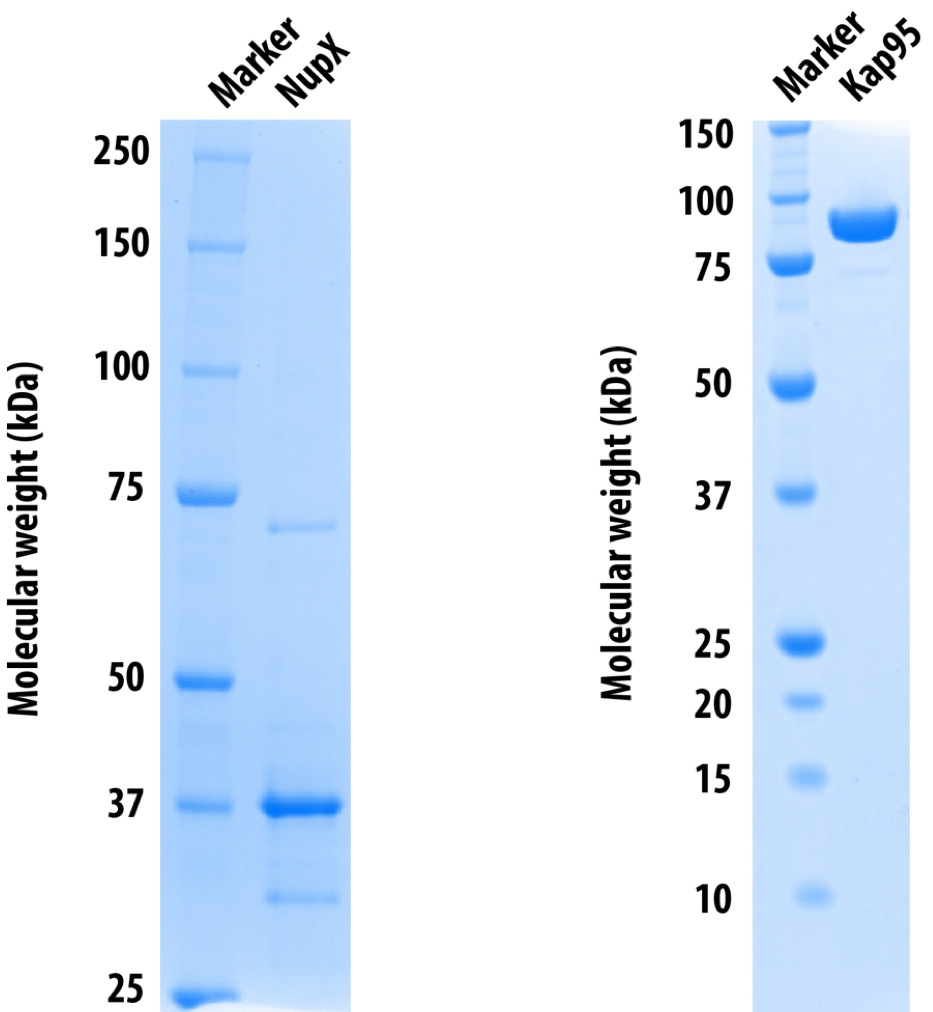
\includegraphics[width=0.5\linewidth]{figures/Figure4.6.png}
	\caption{SDS-PAGE gel shows the band for the 32.5 kDa NupX molecule (left, thick bend running at $\sim$37 kDa) and the 95kDa Kap95 molecule (right) after purification. This experiment was reproduced more than three times yielding similar results.}
	\label{fig:fig.4.8}	
\end{figure}


\subsection{NupX coating of gold surfaces under different concentrations}
\begin{figure}[H]
	\centering
	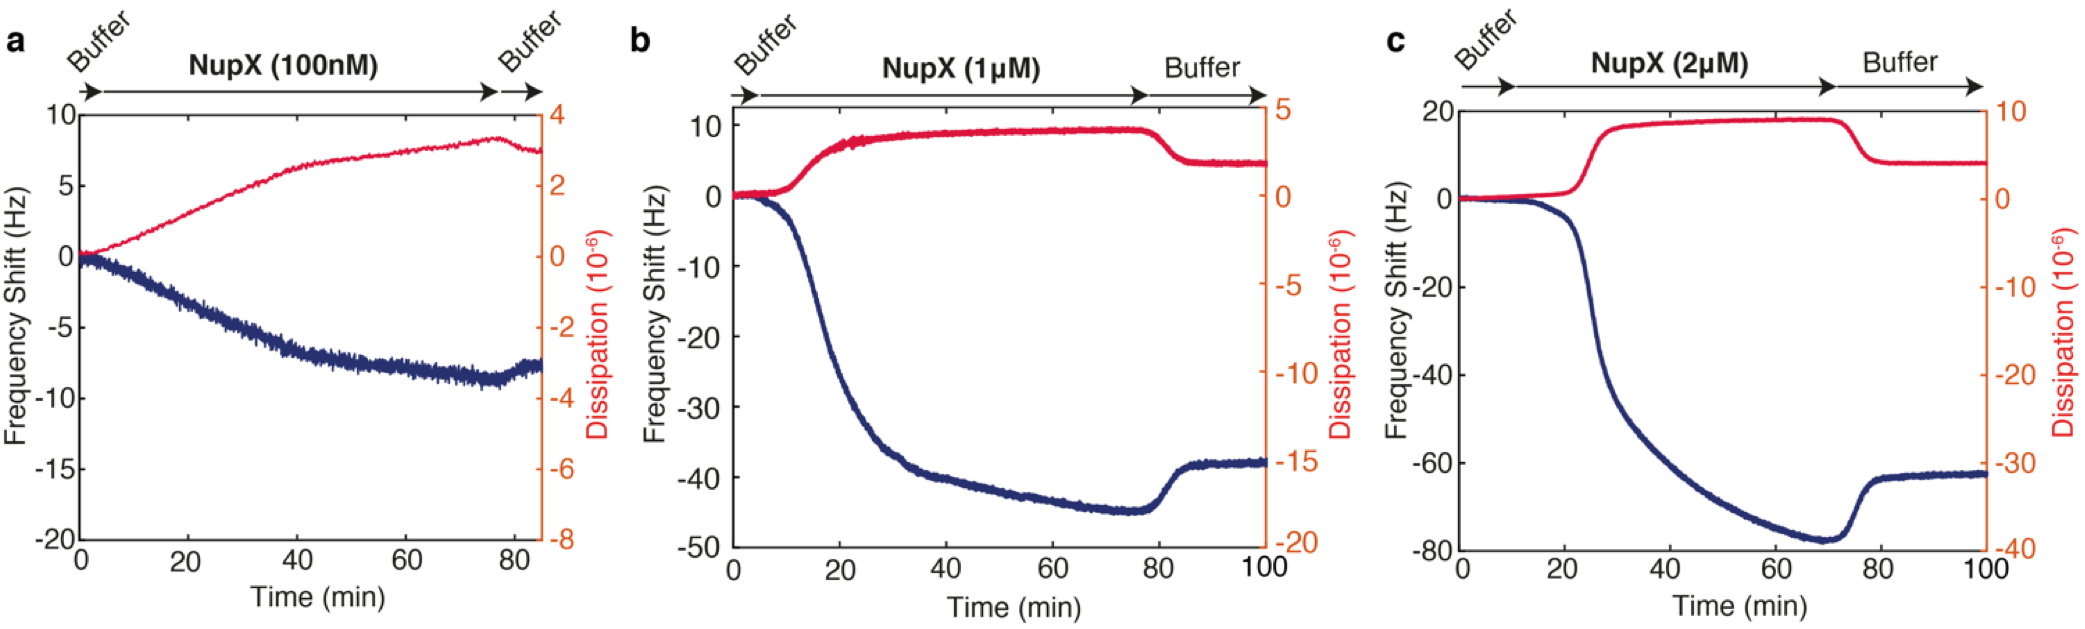
\includegraphics[width=1\linewidth]{figures/Figure4.7.png}
	\caption{Real-time monitoring of NupX-coating of gold-coated quartz chips under concentrations of 100 nM (a), 1 $\mu$M (b), and 2 $\mu$M (c) at constant flow-rate (20 $\mu$L/min), using QCM-D. The slight increase in frequency at the end of the incubation represents the washing step, which induces a subsequent release of nonspecifically bound NupX molecules. The NupX solution included also 1 mM of TCEP in order to reduce the cysteines, which was present during the coating step.}
	\label{fig:fig.4.9}	
\end{figure}

\subsection{SPR measurements of protein- and MUTEG-functionalized chips}
\begin{figure}[H]
	\centering
	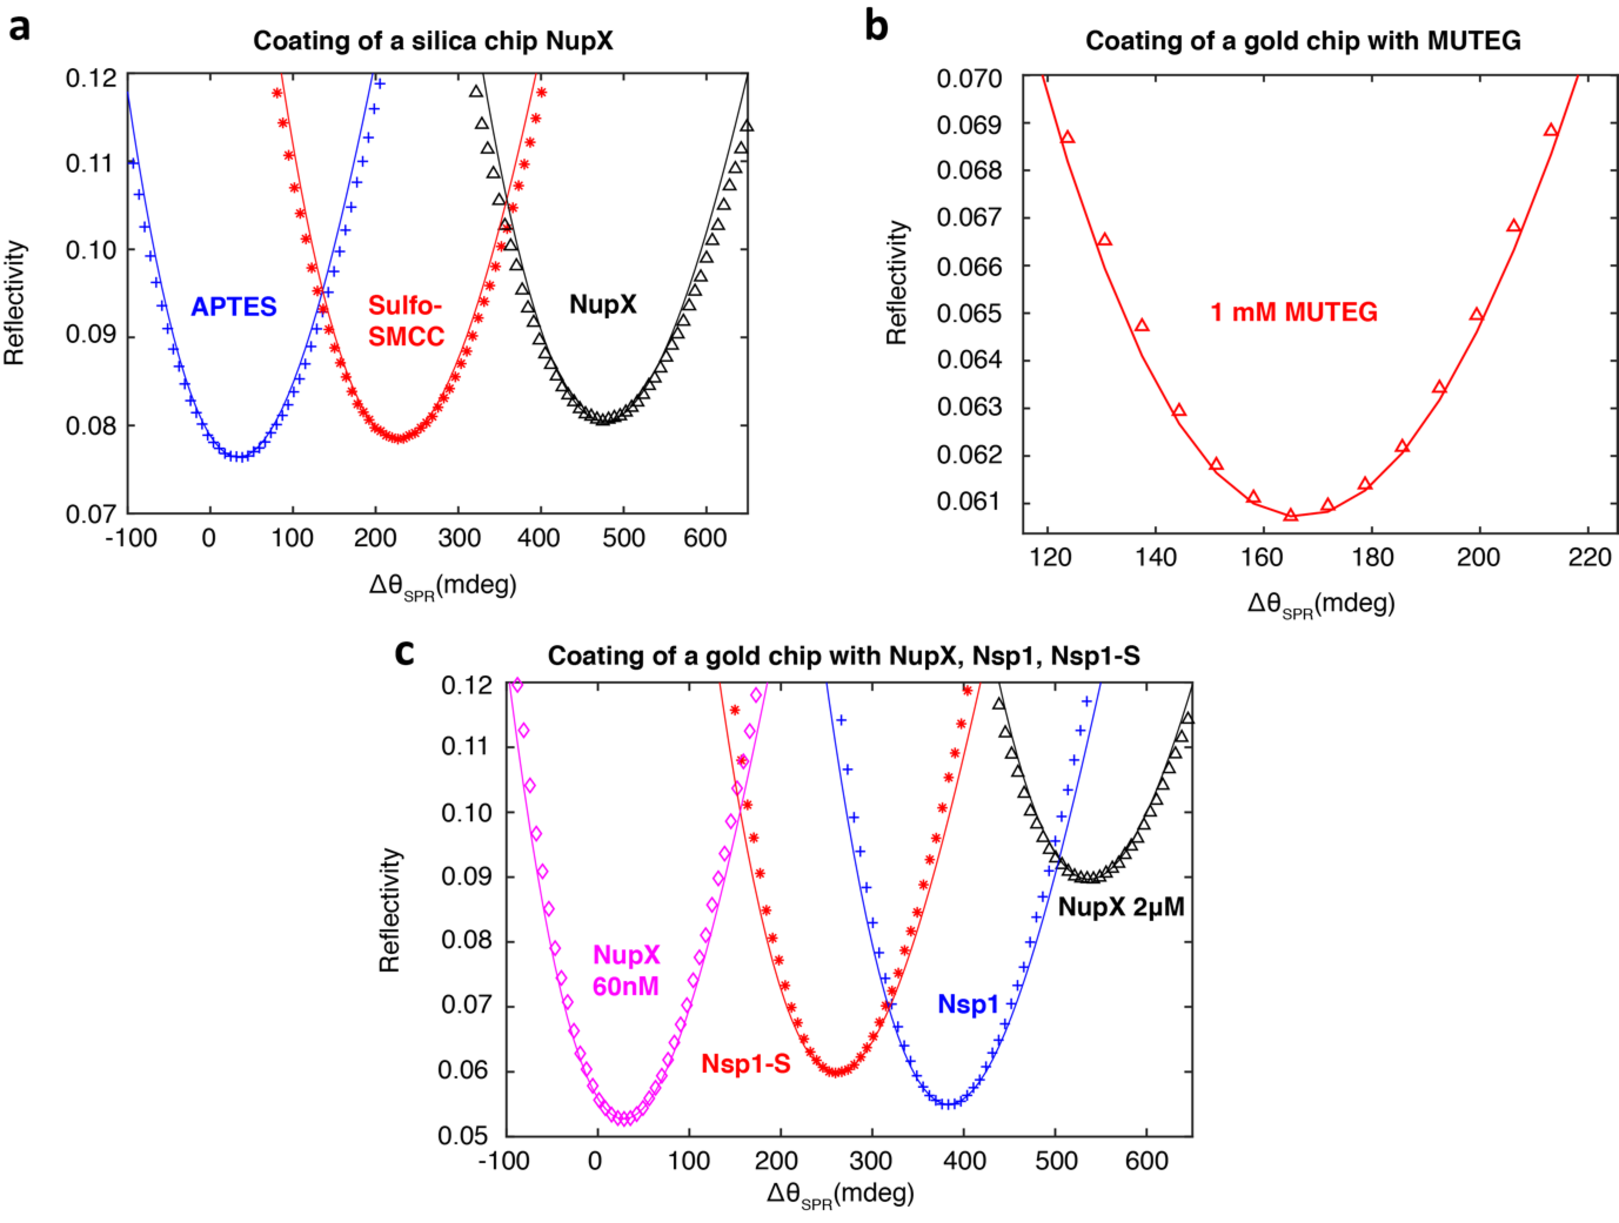
\includegraphics[width=0.7\linewidth]{figures/Figure4.8.pdf}
	\caption{Angular reflectivity spectra of SPR measurements for dried samples in air. a Data for APTES (blue crosses), APTES + Sulfo-SMCC (red asterisks), and APTES + Sulfo-SMCC + NupX (black triangles) on silicondioxide-coated sensors. b Data for MUTEG (380 Da) on gold sensors grafted using 1 mM concentration. c Data for 1 $\mu$M Nsp1 (blue crosses), 1 $\mu$M Nsp1-S (red asterisks), 2 $\mu$M (black triangles) and 60 nM NupX (pink diamonds) on gold sensors. $\Delta\theta_{SPR}$ denotes the angular shift in millidegrees of the resonance angle. Solid lines show Fresnel model fits (which are offset in the $y$-direction to match the measurement reflectivity minima), which are used to determine the thickness of each adlayer.}
	\label{fig:fig.4.10}	
\end{figure}
\subsection{Passivation of NupX-covered Au-surfaces using MUTEG}
\begin{figure}[H]
	\centering
	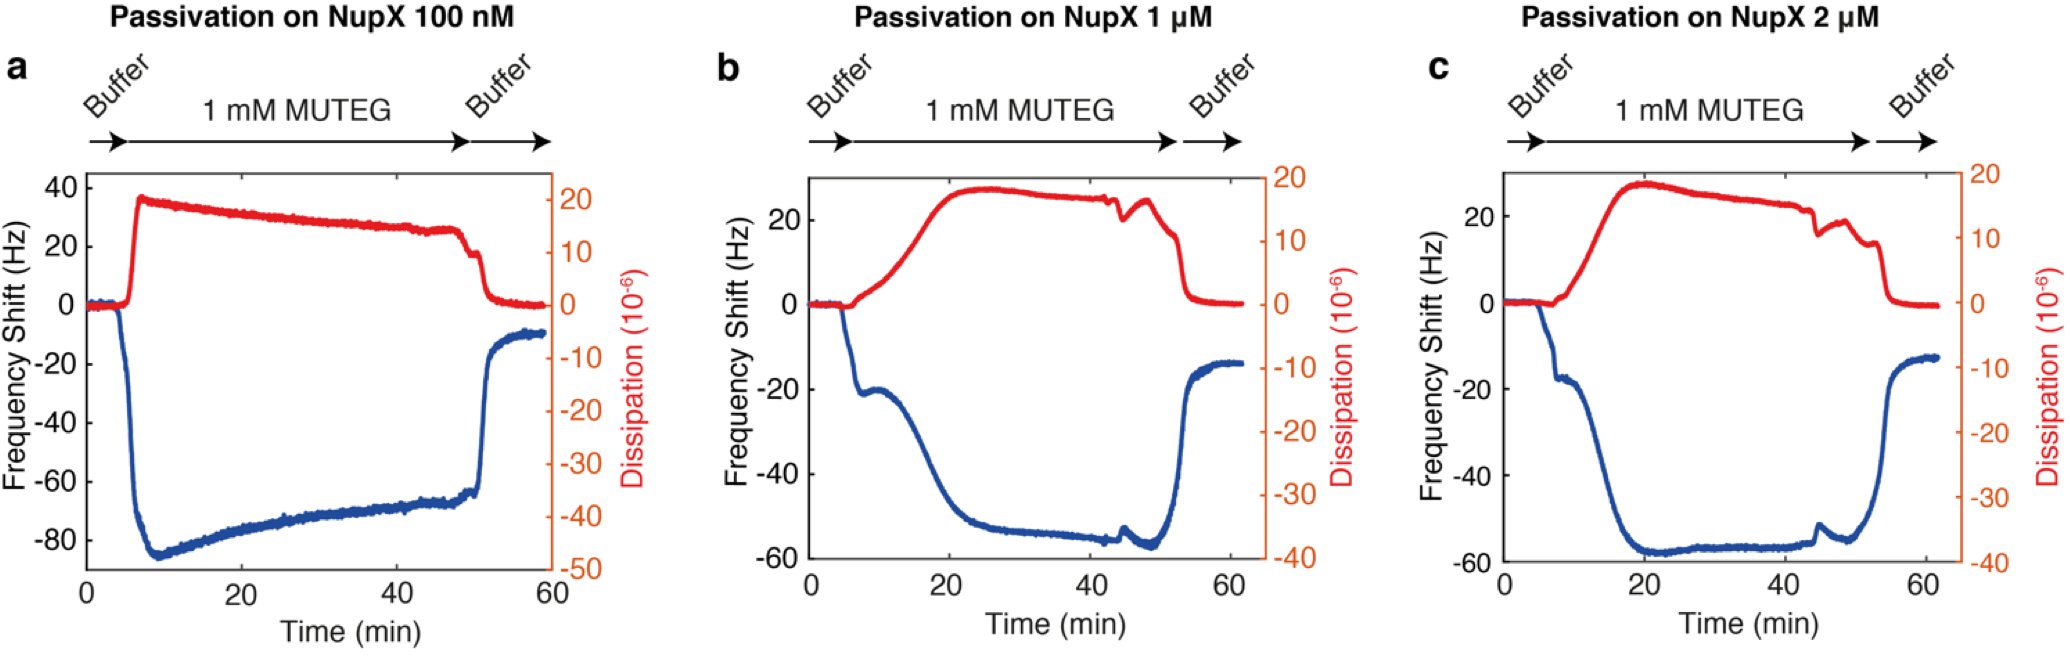
\includegraphics[width=1\linewidth]{figures/Figure4.9.png}
	\caption{Real-time monitoring of 1 mM MUTEG binding to gold chips that were pre-functionalized with NupX at NupX concentrations of 100 nM (a), 1 $\mu$M (b), and 2 $\mu$M (c) at constant flow-rate (20 $\mu$L/min), using QCM-D. Note that final dissipation shifts were all close to zero, while (negative) frequency shifts were found in the range of $\sim$10-14 Hz, indicating the formation of a thin monolayer. The MUTEG solution included also 10 mM of TCEP in order to reduce the thiols, which was present during the coating step (same for Fig.\ref{fig:fig.4.10}a).}
	\label{fig:fig.4.11}	
\end{figure}

\subsection{Kap95 binding to passivated gold QCM-D chip}
\begin{figure}[H]
	\centering
	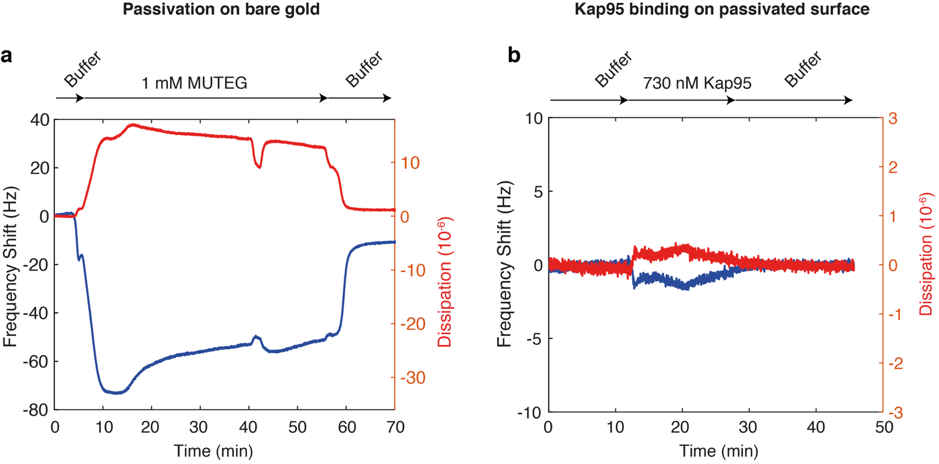
\includegraphics[width=1\linewidth]{figures/Figure4.10.png}
	\caption{Real-time monitoring of Kap95 interacting with a MUTEG-passivated gold surface. a, Frequency shift over time upon flushing of 1 mM of 1-mercapto-11-undecylte-tra(ethyleneglycol) (MUTEG) onto a gold surface. From an independent measurement using SPR (Fig.\ref{fig:fig.4.10}b) where the same incubation time and concentration were used, the MUTEG coating of a bare gold surface yielded a dense monolayer with a $0.59\pm0.01$ nm average grafting distance. b, Frequency shift over time upon flushing of 730 nM of Kap95 to a MUTEG-passivated gold layer. Only minor interactions ($<2$ Hz) were detected.}
	\label{fig:fig.4.12}	
\end{figure}
\subsection{Kap95 dissociation from NupX by 0.2 M NaOH}
\begin{figure}[H]
	\centering
	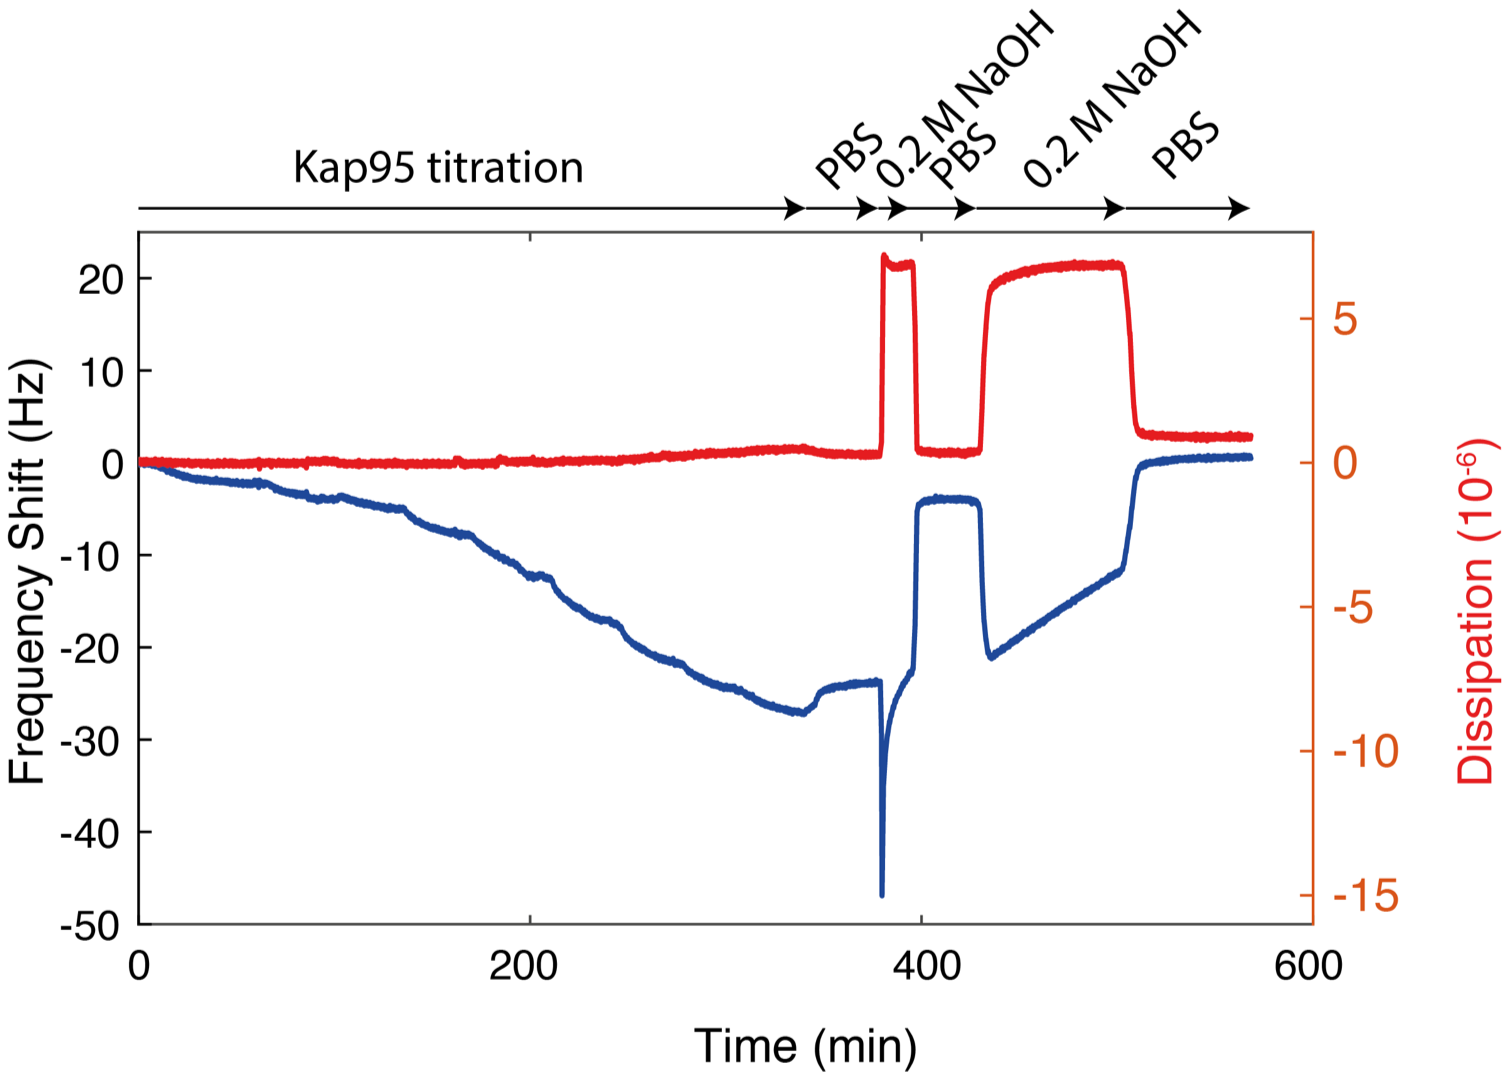
\includegraphics[width=0.7\linewidth]{figures/Figure4.11.png}
	\caption{Real-time monitoring of Kap95 interacting with a NupX-coated surface with subsequent dissociation upon flushing of 0.2 M NaOH. }
	\label{fig:fig.4.13}	
\end{figure}
\subsection{Kap95 vs BSA binding to different NupX-coated gold surfaces}
\begin{figure}[H]
	\centering
	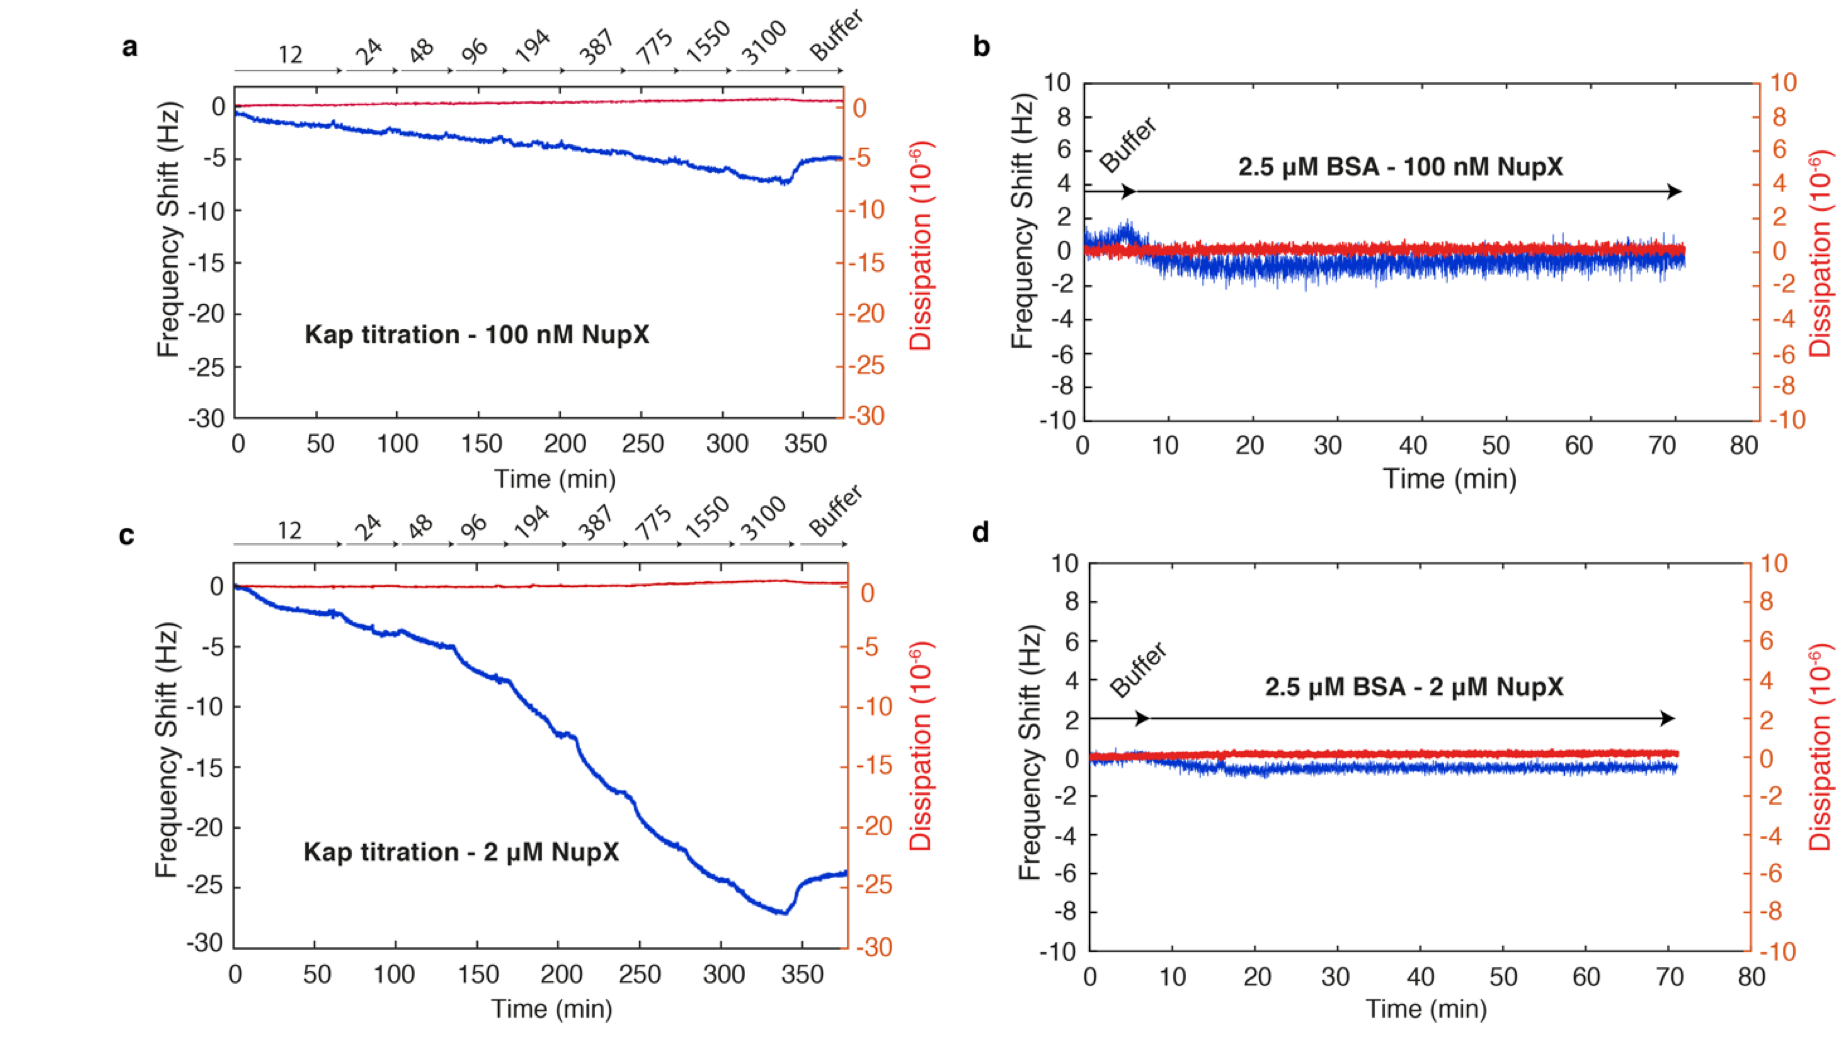
\includegraphics[width=0.8\linewidth]{figures/Figure4.12.png}
	\caption{Real-time monitoring of $\sim$10-3000 nM Kap95 and 2500 nM BSA binding to gold chips functionalized with NupX at a concentration of 100 nM (a-b, respectively) and 2 $\mu$M (c-d, respectively), at constant flow-rate (20 $\mu$L/min), using QCM-D.}
	\label{fig:fig.4.14}	
\end{figure}
\subsection{Testing the stability of NupX coatings against milliQ and 50\% pure ethanol}
\begin{figure}[H]
	\centering
	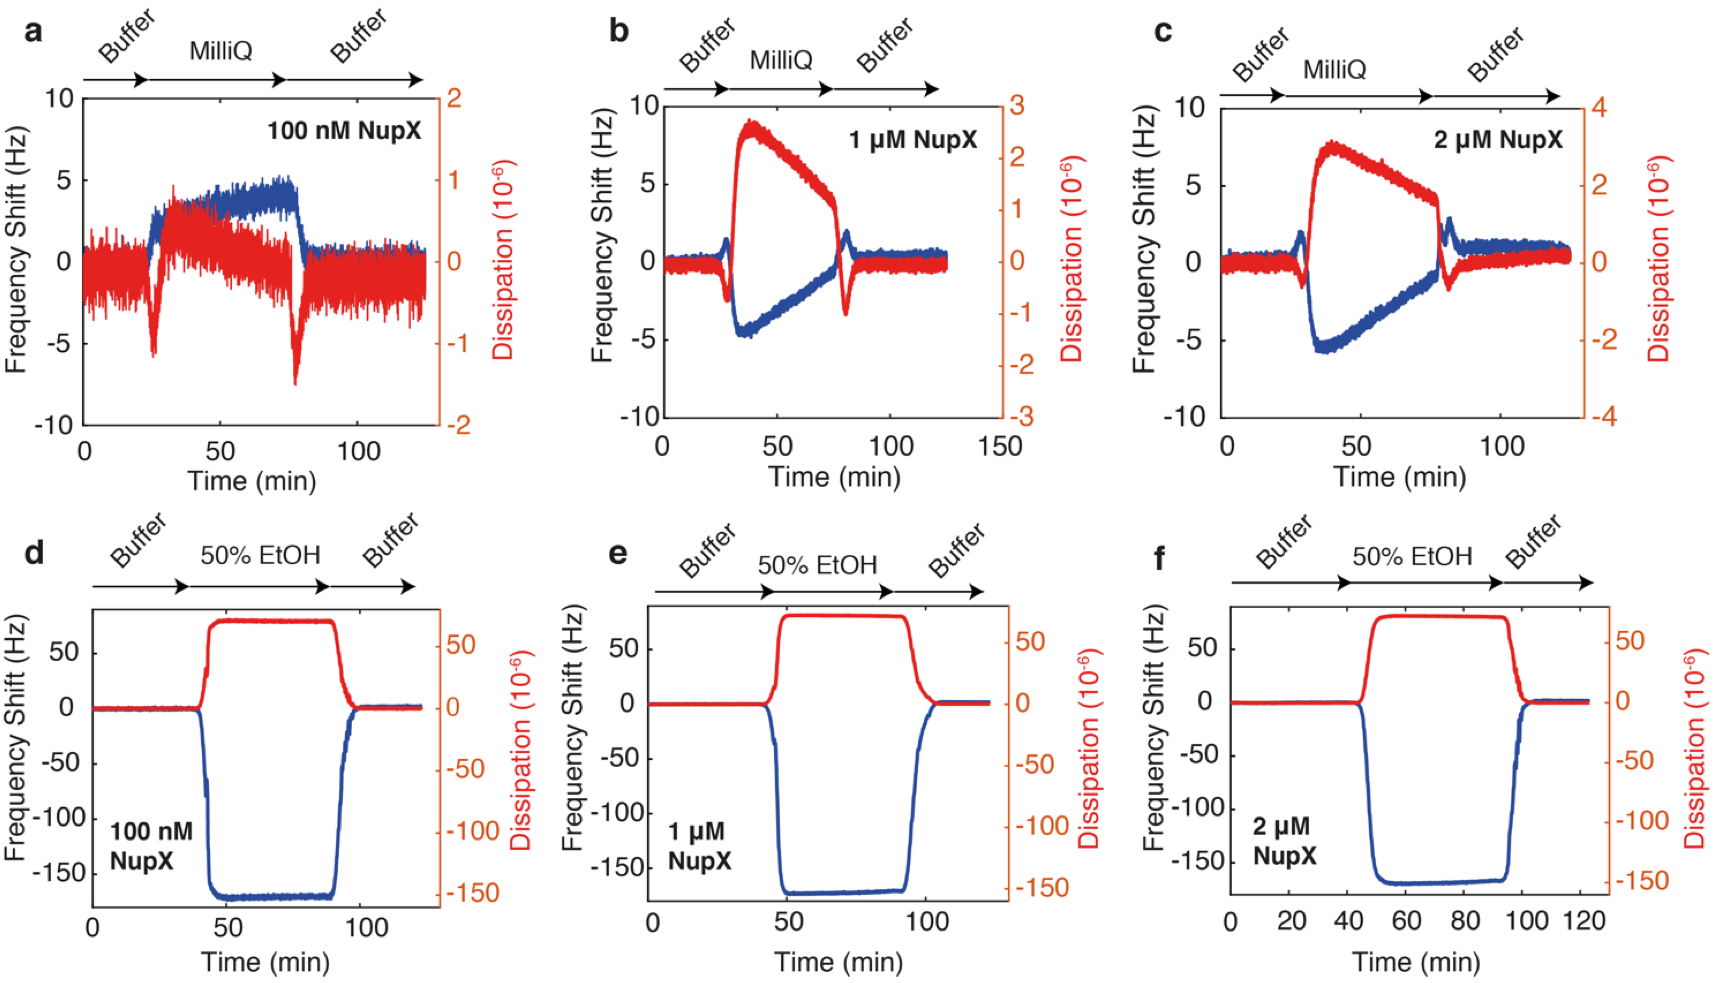
\includegraphics[width=0.8\linewidth]{figures/Figure4.13.png}
	\caption{Real-time monitoring of milliQ and 50\% pure ethanol rinsing of gold surfaces that were pre-coated with NupX and subsequently passivated with 1 mM MUTEG, at different NupX concentrations of 100 nM (a,d, respectively), 1 $\mu$M (b,e, respectively), and 2 $\mu$M (c,f, respectively), at constant flow-rate (20 $\mu$L/min), using QCM-D. Note that final frequency and dissipation shifts are all close to zero, indicating that our protein and MUTEG layers are stably bound to the gold surface.}
	\label{fig:fig.4.15}	
\end{figure}
\subsection{Dissipation-to-Frequency ratio change upon QCM-D coating}
\begin{figure}[H]
	\centering
	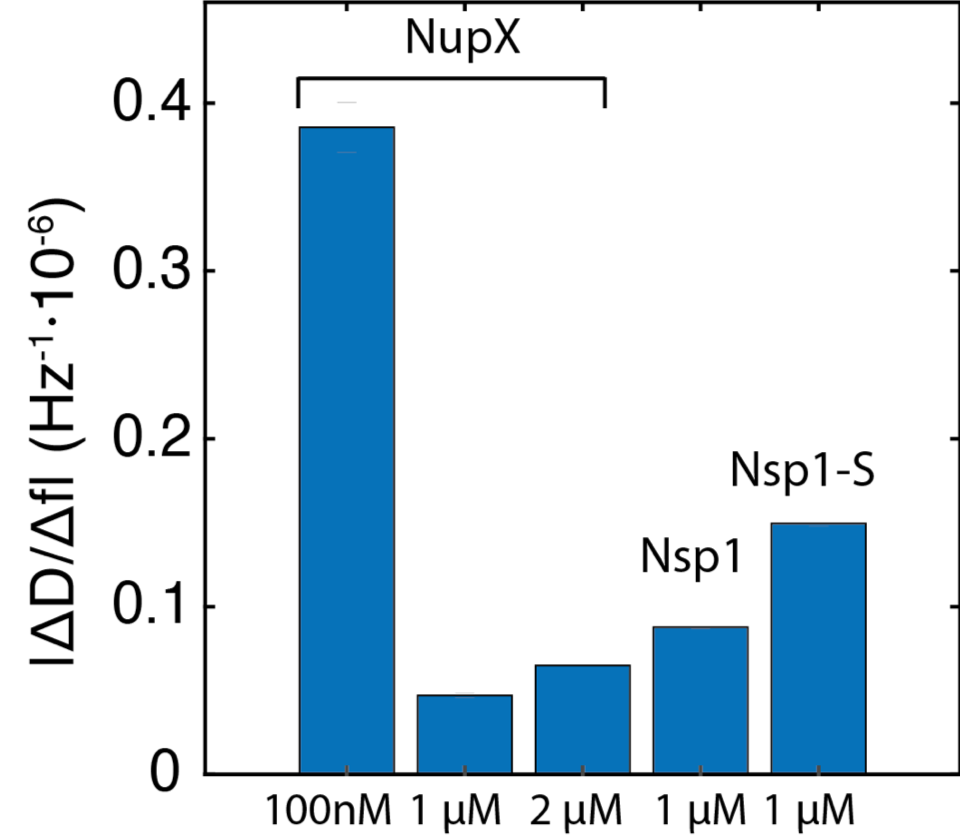
\includegraphics[width=0.5\linewidth]{figures/Figure4.14.png}
	\caption{Dissipation-to-frequency ratio $\Delta D_5/\Delta f_5/5$ for NupX (with concentrations as in Figure \ref{fig:fig.4.7}), Nsp1, Nsp1-S coating of a gold-coated quartz chip. When comparing the 3 proteins (NupX, Nsp1, and Nsp1-S) for the same incubation concentration of 1 $\mu$M, NupX produced the lowest dissipation-to-frequency ratio, consistent with the higher hydrophobic character of GLFG-type Nups (\emph{e.g.} Nup98 [1]), and hence of NupX, as compared to FXFG-Nups. Note that these $\Delta D_5/\Delta f_5/5$ values are for the FG-Nup films only, \emph{i.e.} prior MUTEG passivation.}
	\label{fig:fig.4.16}	
\end{figure}
\subsection{Dissipation-to-frequency ratio of a NupX layer upon increasing Kap95 concentration}
\begin{figure}[H]
	\centering
	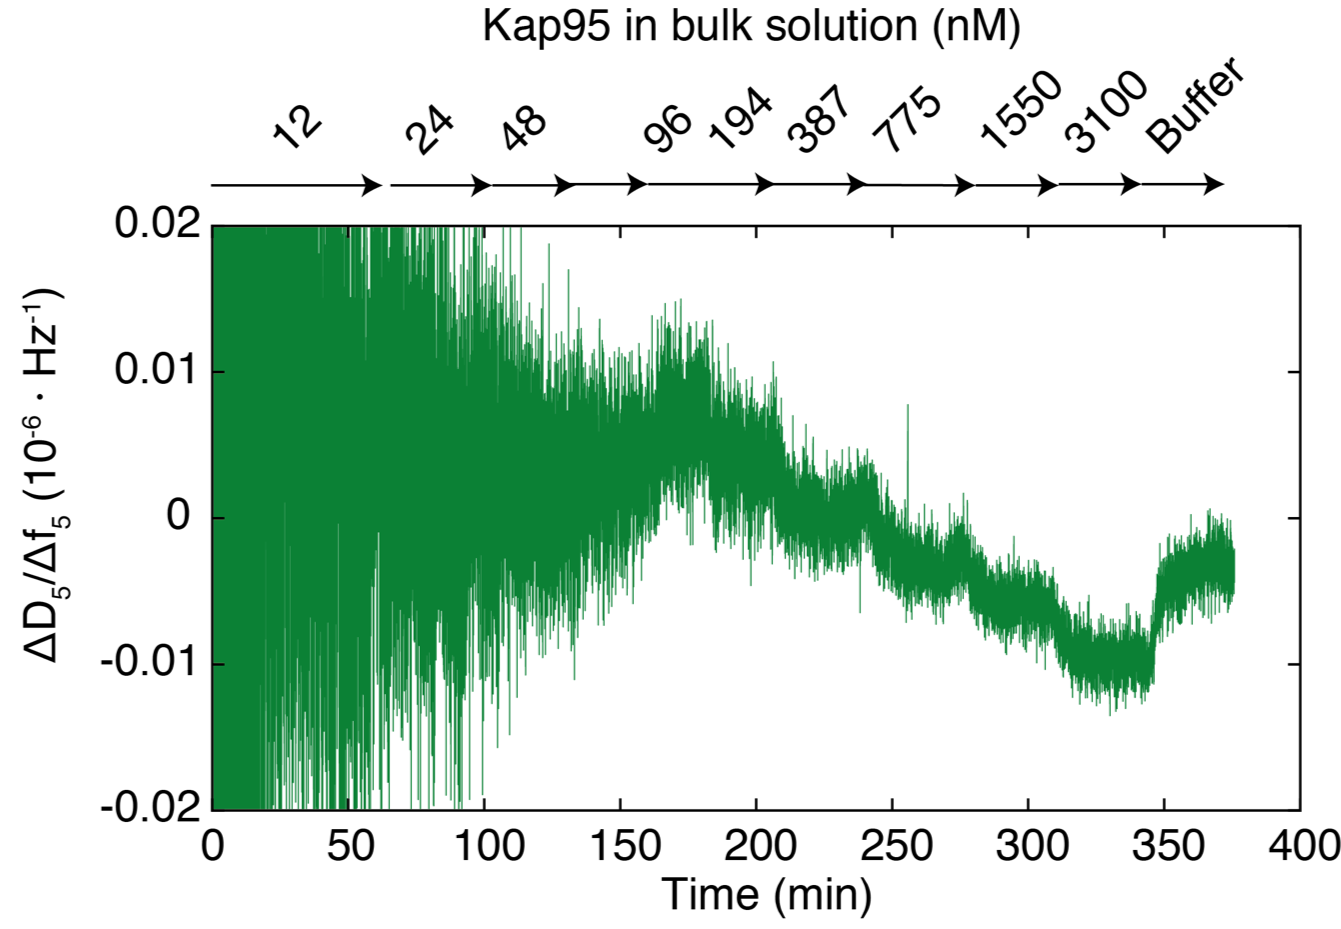
\includegraphics[width=0.7\linewidth]{figures/Figure4.15.png}
	\caption{Dissipation-to-frequency ratio $\Delta D_5/\Delta f_5/5$ for Kap95 absorption to a NupX-coated surface for increasing concentrations (from 12 nM to 3100 nM).}
	\label{fig:fig.4.17}	
\end{figure}
\subsection{Coarse-grained simulations of cargo adsorption in a NupX brush with a 5.7 nm grafting distance}
\begin{figure}[H]
	\centering
	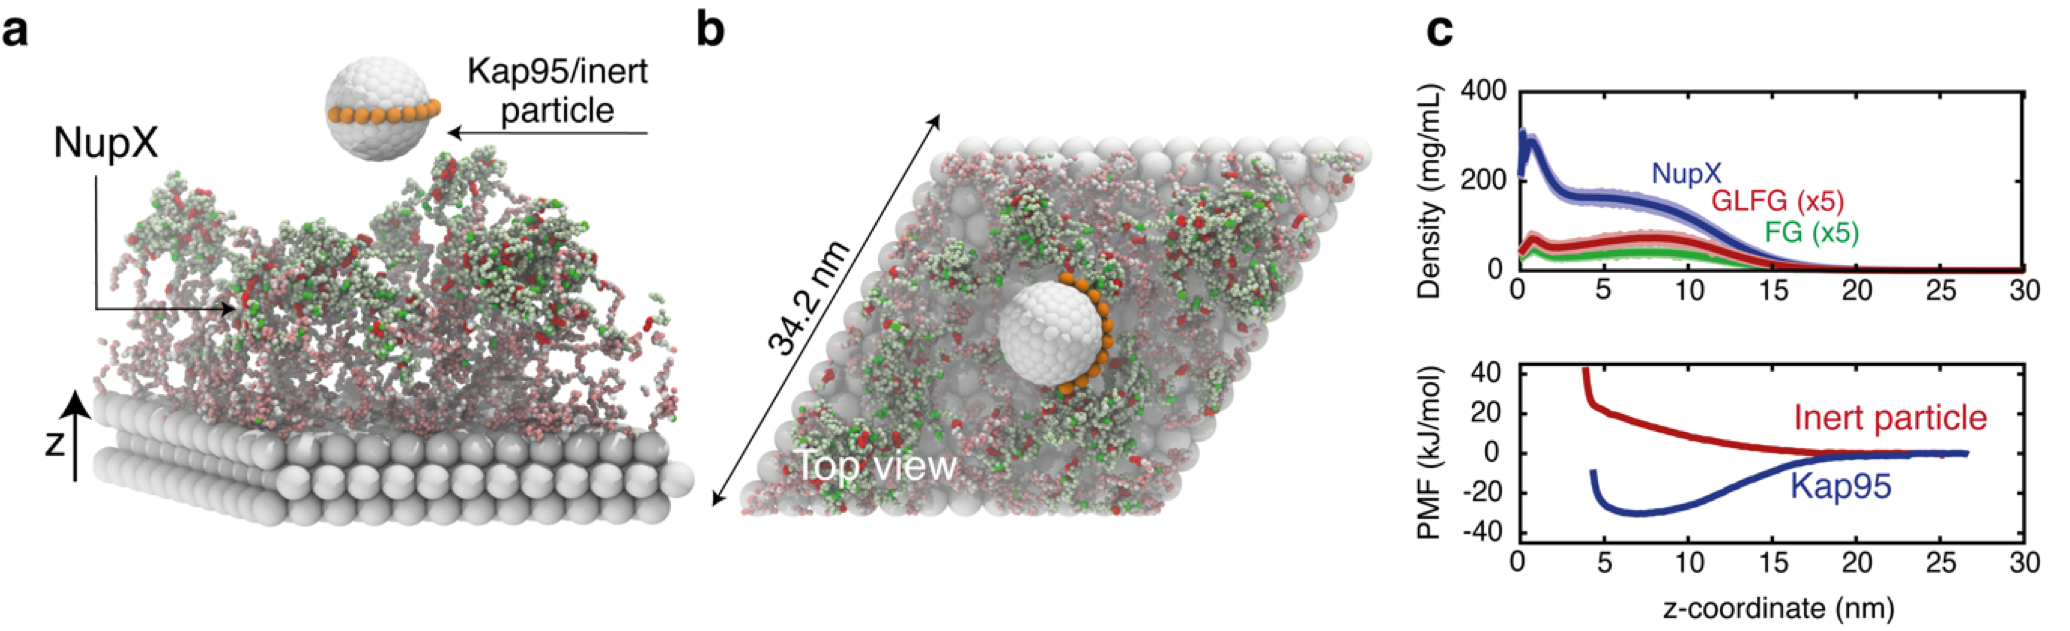
\includegraphics[width=0.9\linewidth]{figures/Figure4.16.png}
	\caption{NupX brush system, simulated for a grafting distance of 5.7 nm. a,b Snapshots of the simulations (see also: Figure \ref{fig:fig.4.2}h). c, Top panel: Time and laterally averaged protein density distributions for the NupX brushes and for the two different types of FG motifs present inside the NupX brushes. The density profiles of the GLFG and FG motifs within the NupX brush are multiplied by 5 for clarity of display. Dark central lines and light shades indicate the mean and standard deviation in density profiles, respectively. These measures were obtained by averaging over the density profiles of trajectory windows 50 ns in length (N=60).  A high-density region (up to a maximum of 300 mg/mL) forms near the attachment sites of the NupX to the surface ($z=0$ to 2 nm). Further away from the scaffold, the protein density remains at a constant value of $\sim$170 mg/mL up to a distance of $\sim$8 nm, after which it decays. FG and GLFG motifs predominantly localize near the transitioning point (8 nm). Bottom panel: Free-energy profiles (PMF-curves) of the center of mass of the model Kap95 and inert particle along the $z$-coordinate, where $z=0$ coincides with the substrate. The PMF-curves originate from a $z$-value where the distance between the center of mass of either particle and the substrate approaches one half of the former’s diameter. The difference in sign between the PMF-curves of both particles indicates a strong preferential absorption of the model Kap95 to NupX brushes and a repulsive interaction of the inert particle. Compared to the brush with a lower grafting distance (see Figs. \ref{fig:fig.4.2}h,i in the main text), the repulsion and adsorption are less strong, which is due to the decrease in the density of the NupX brush and FG/GLFG-motifs, respectively (see c top panel).}
	\label{fig:fig.4.18}	
\end{figure}
\subsection{Model Kap95 particle}
\begin{figure}[H]
	\centering
	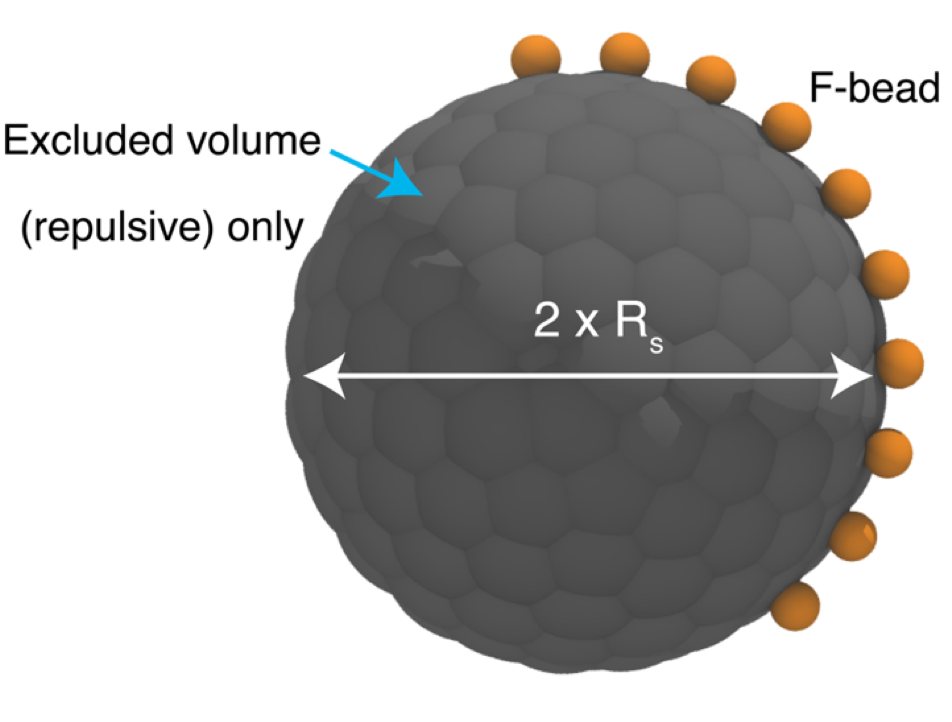
\includegraphics[width=0.4\linewidth]{figures/Figure4.17.png}
	\caption{The computational model of the Kap95 particle used in this work, rendered using VMD2. The Kap95 (and the inert particle) consists of sterically repulsive beads (\emph{i.e.}, only repulsive excluded volume interactions with its surroundings, here shown in dark grey) arranged in a geodesic shell. In the case of the Kap95 particle a strip of 10 hydrophobic binding sites (brown-orange) is placed on the surface, and the net charge ($-$43e) is distributed equally over all the surface beads. Binding sites are modeled as Phenylalanine beads and are spaced 1.3 nm apart on an arc. Phe-beads are the most hydrophobic particle type in our 1-BPA model. The diameter of Kap95 is equal to two times the Stokes radius (see Table \ref{tab:table4.1}).}
	\label{fig:fig.4.19}	
\end{figure}
\subsection{Conductance decrease upon NupX-coating of solid-state nanopores}
\begin{figure}[H]
	\centering
	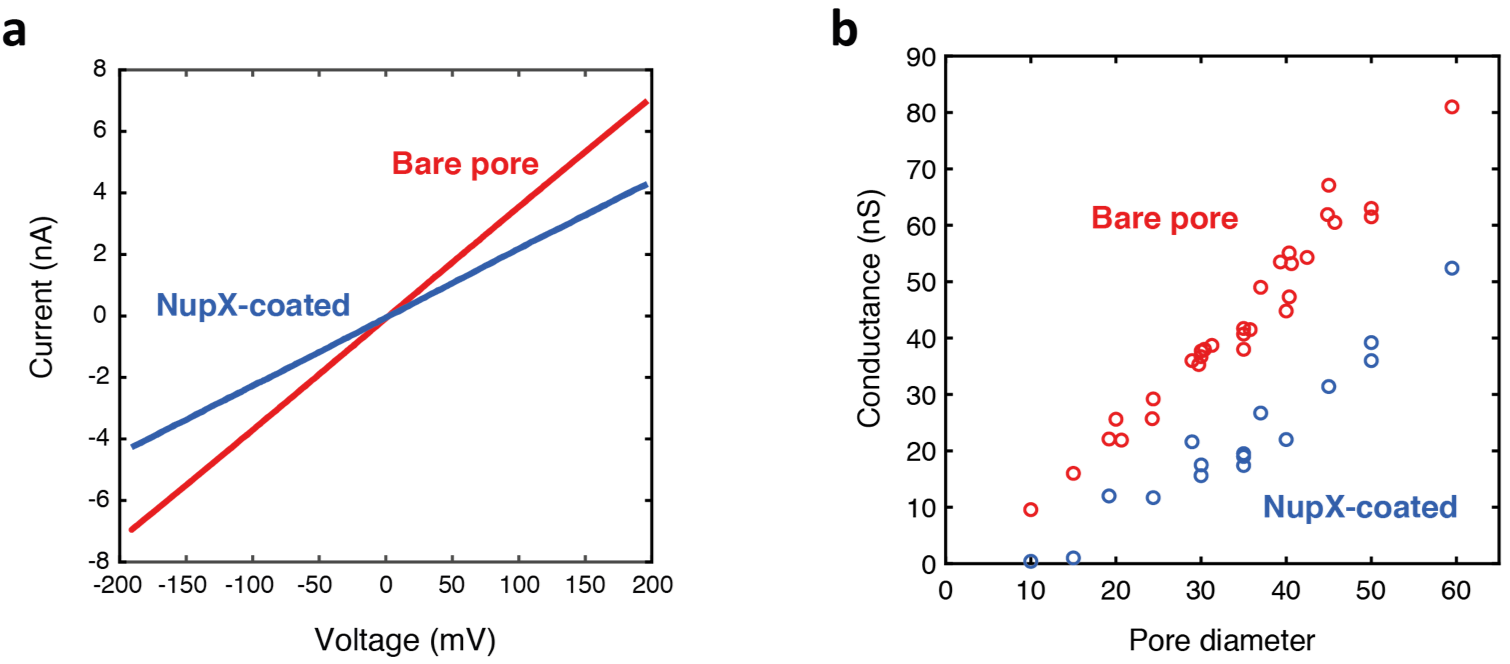
\includegraphics[width=1\linewidth]{figures/Figure4.18.png}
	\caption{NupX-coating of solid-state nanopores. a, I-V characteristics for a bare (red) and NupX-coated (blue) 30 nm pore. b, Ionic conductance of differently sized nanopores over a range of 10-60 nm is plotted vs diameter for bare (red) and coated (blue) pores.}
	\label{fig:fig.4.20}	
\end{figure}

\subsection{Current Power Spectral Density before and after NupX-coating}
\begin{figure}[H]
	\centering
	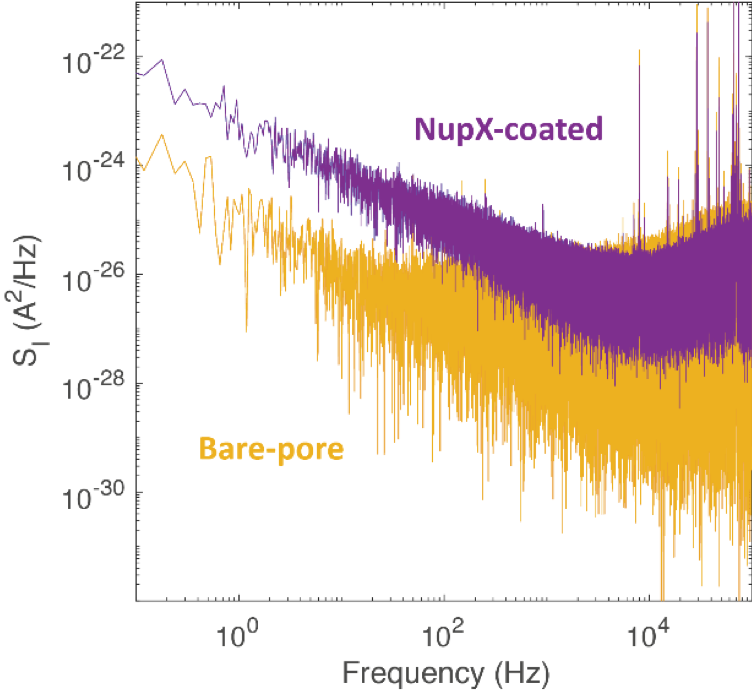
\includegraphics[width=0.5\linewidth]{figures/Figure4.19.png}
	\caption{Power Spectral Density of the ionic current noise before (yellow curve) and after (purple) NupX-coating for a 30 nm pore. }
	\label{fig:fig.4.21}	
\end{figure}
\subsection{Selectivity measurements through different pore sizes (30 nm, 35 nm and 60 nm)}
\begin{figure}[H]
	\centering
	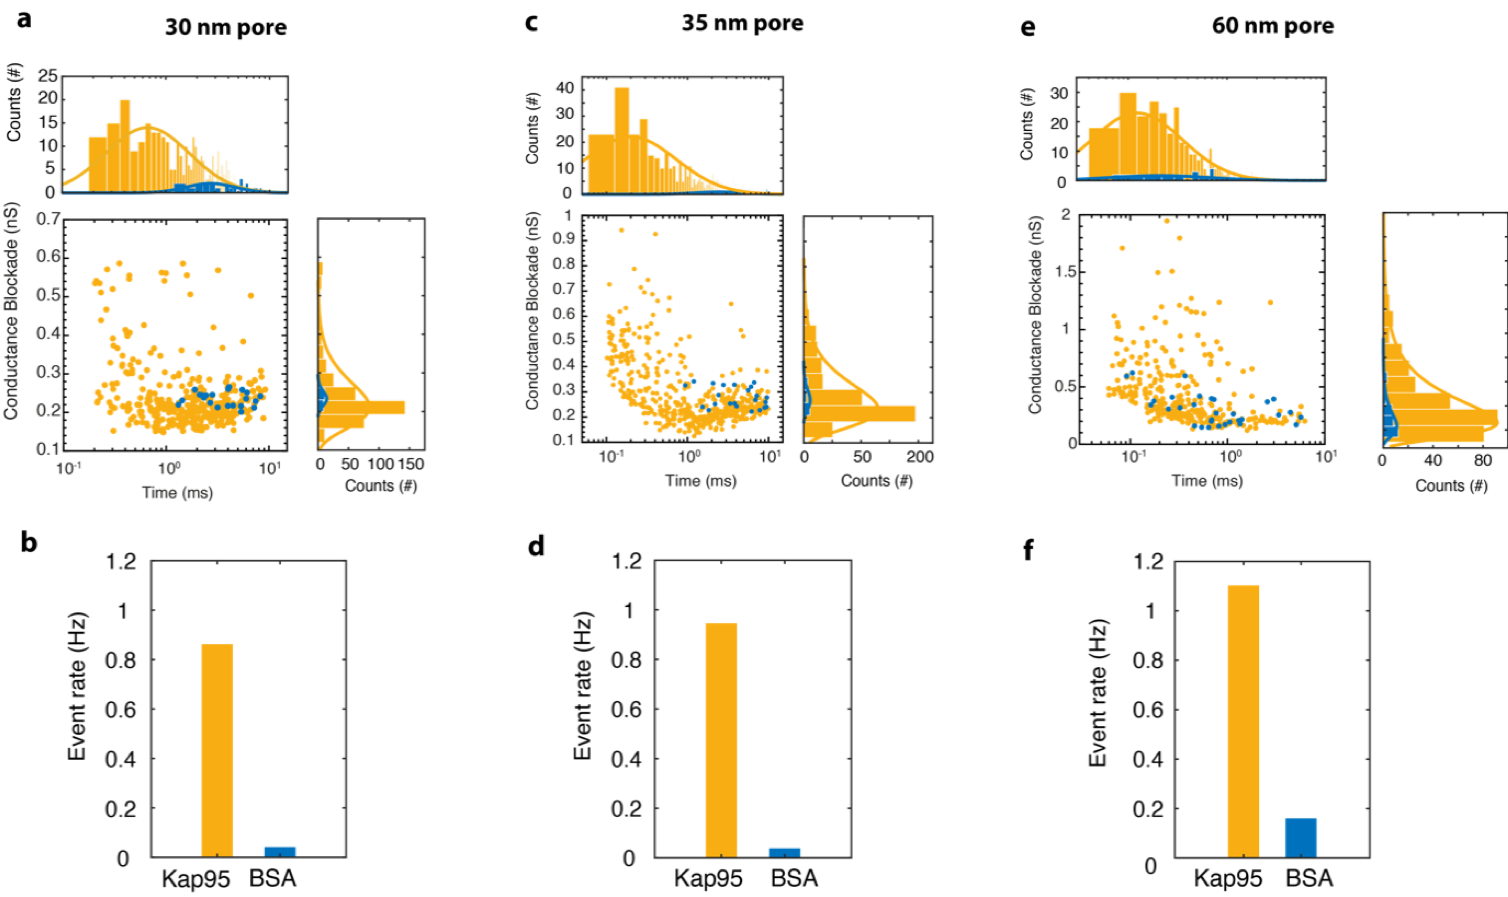
\includegraphics[width=1\linewidth]{figures/Figure4.20.png}
	\caption{Selectivity measurements on NupX-coated pores of different sizes. Scatter plots show event distributions for translocations of 2.8 $\mu$M BSA and 450 nM Kap95 under 100 mV applied bias, in 150 mM KCl, pH 7.4 buffer. a-b, Scatter plot and bar plot showing (a) conductance blockades (0.24$\pm$0.07 nS for Kap95, 0.24$\pm$0.02 nS for BSA; errors in s.d.) vs dwell times (2.4$\pm$0.4 ms for Kap95, 4.2$\pm$1.2 ms for BSA; errors in s.e.m.) (b) and event rates (0.9 Hz for Kap95, 0.04 Hz for BSA) for translocations of Kap95 (N=369) and BSA (N=22) through a NupX-coated 30 nm pore. c-d, Scatter plot and bar plot showing (c) conductance blockades (0.3$\pm$0.1 nS for Kap95, 0.28$\pm$0.04 nS for BSA; errors in s.d.) vs dwell times (2.5$\pm$0.2 ms for Kap95, 5.2$\pm$0.9 ms for BSA; errors in s.e.m.) and (d) event rates (0.95 Hz for Kap95, 0.04 Hz for BSA) for translocations of Kap95 (N=482) and BSA (N=23) through a NupX-coated 35 nm. e-f, Scatter plot and bar plot showing (e) conductance blockades (0.45$\pm$0.03 nS for Kap95, 0.30$\pm$0.02 nS for BSA; errors in s.d.) vs dwell times (0.65$\pm$0.05 ms for Kap95, 1.6$\pm$1.3 ms for BSA; errors in s.e.m.) and (f) event rates (1.1 Hz for Kap95, 0.04 Hz for BSA) for translocations of Kap95 (N=314) and BSA (N=32) through a NupX-coated 60 nm pore.  }
	\label{fig:fig.4.22}	
\end{figure}
\newpage
\subsection{Event rate of Kap95 translocation through NupX-coated pores vs Kap95 concentration}
\begin{figure}[H]
	\centering
	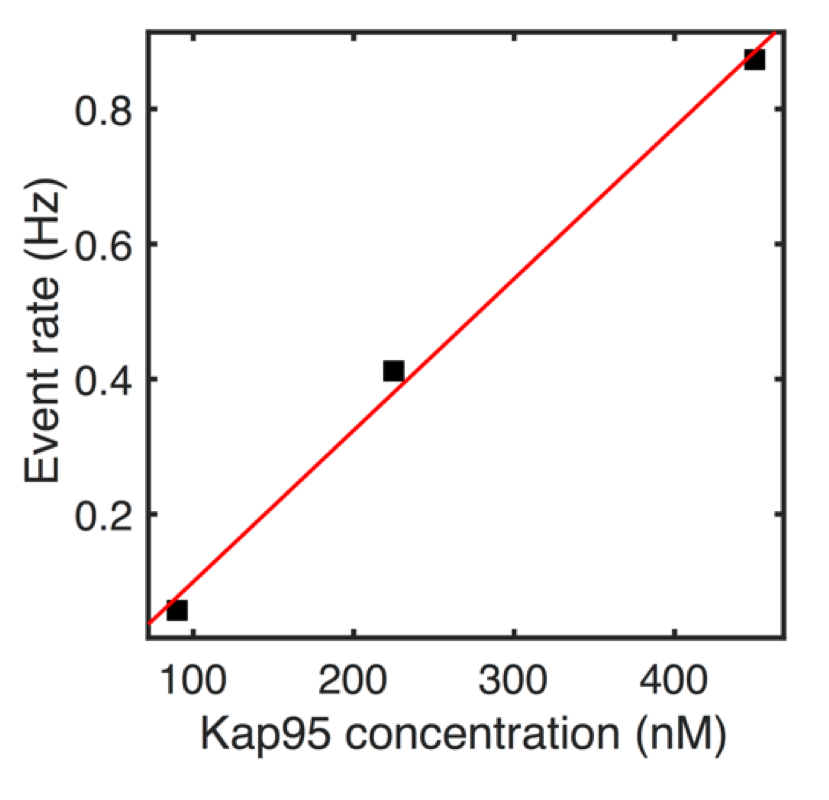
\includegraphics[width=0.4\linewidth]{figures/Figure4.21.png}
	\caption{Event rate of translocation of Kap95 molecules through a NupX-coated pore, at increasing concentrations from 90 nM, 225 nM, to 450 nM. The translocation frequency increases linearly with concentration, as expected.}
	\label{fig:fig.4.23}	
\end{figure}
\subsection{Density distributions of NupX for different grafting densities}
\begin{figure}[H]
	\centering
	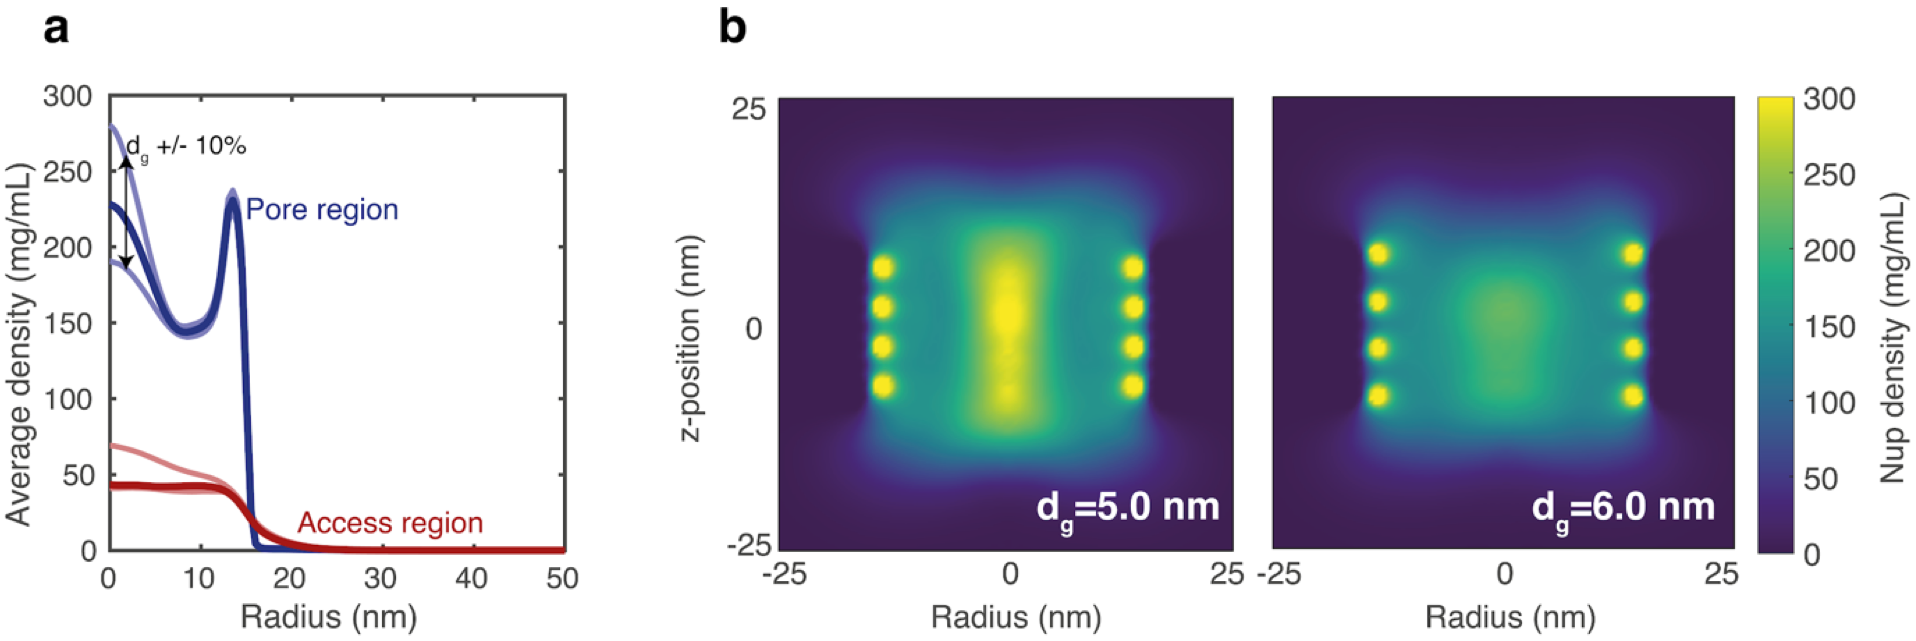
\includegraphics[width=1\linewidth]{figures/Figure4.22.png}
	\caption{Sensitivity of the average pore and access region protein densities against a change in grafting distance $d_g$. a, Upon increase resp. decrease of the grafting distance with approx. 10\% (6.0/5.0 nm as compared to 5.5 nm used for SiN in the main text), we observe a corresponding decrease ($-17$\%) and increase ($+22$\%) in the maximal pore region density (light blue and dark blue curves, resp.). The maximal access region density (red) is only sensitive to a decrease in grafting distance, where a 10\% decrease in grafting distance yields a large density increase of $+60$\% due to NupX proteins being expelled from the pore region (light red). b, Axi-radial density distributions of 30 nm NupX-lined nanopores upon an approximate 10\% decrease (left panel) or increase (right panel) in grafting distance. The high-density region towards the central axis of the nanopore increases in density and extends over a larger range in the $z$-direction when the grafting distance is decreased, whereas the opposite occurs for an increase in grafting distance. The overall morphology of the NupX-meshwork in the nanopore remains consistent under an increase of approximately 10\% in grafting distance.}
	\label{fig:fig.4.24}	
\end{figure}
\subsection{Density distributions of NupX in the access region}
\begin{figure}[H]
	\centering
	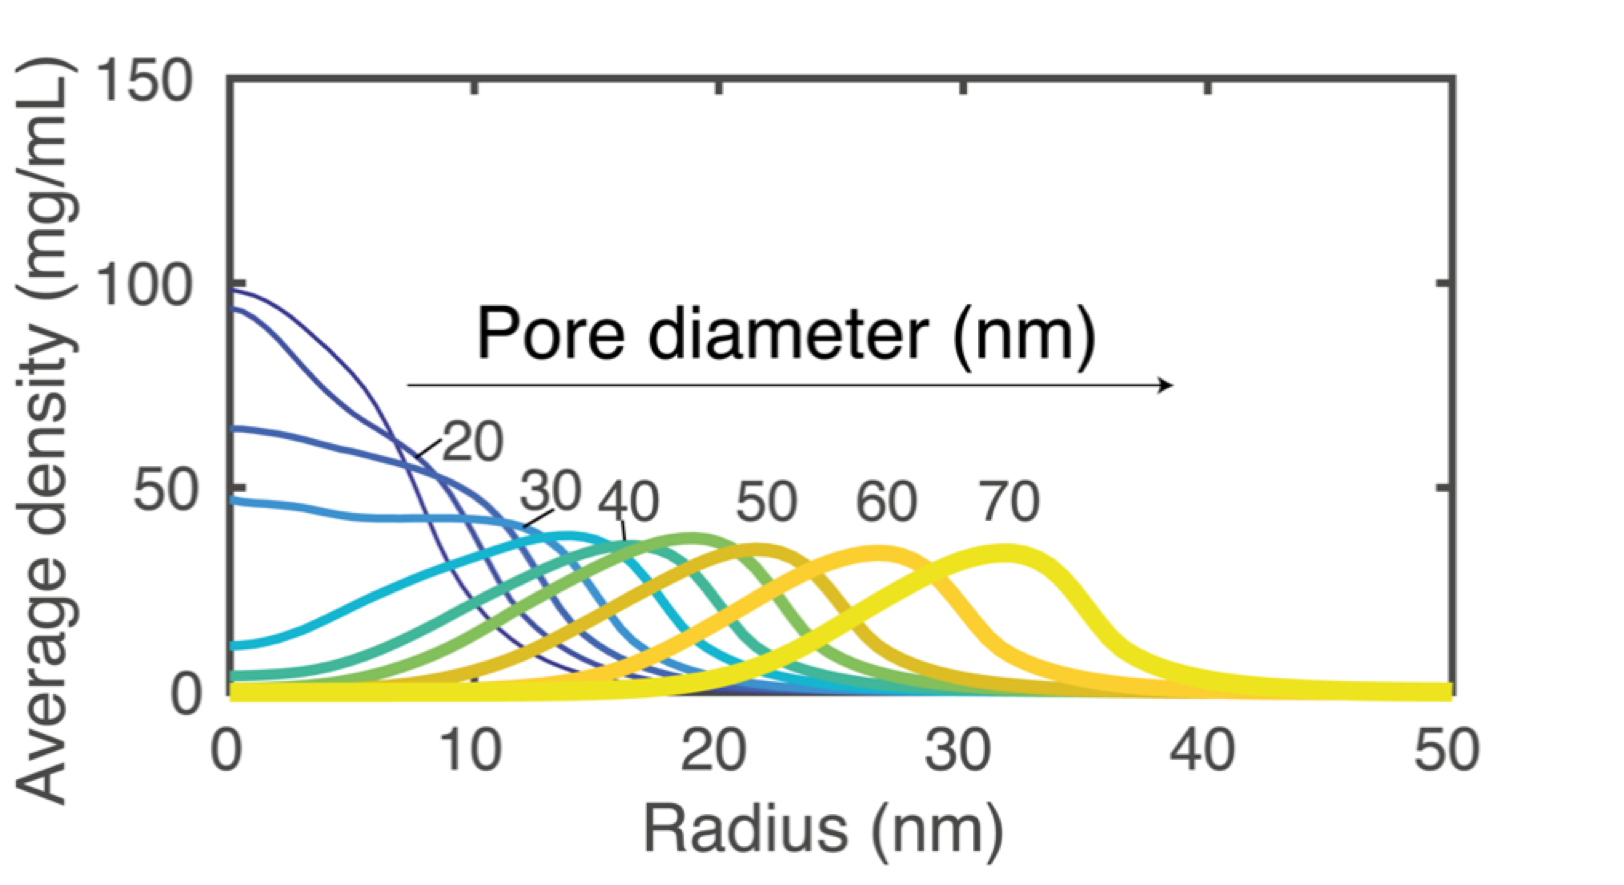
\includegraphics[width=0.8\linewidth]{figures/Figure4.23.png}
	\caption{Access region densities for NupX-lined nanopores with diameters ranging from 15 nm to 70 nm. Lighter colors and increasing line thicknesses indicate larger diameter pores. A preferred localization of NupX proteins towards the central axis of the pore region occurs for a pore diameter of 30 nm and smaller.}
	\label{fig:fig.4.25}	
\end{figure}
\subsection{Density distribution of NupX in a 30 nm pore in the presence of Kap95 molecules}
\begin{figure}[H]
	\centering
	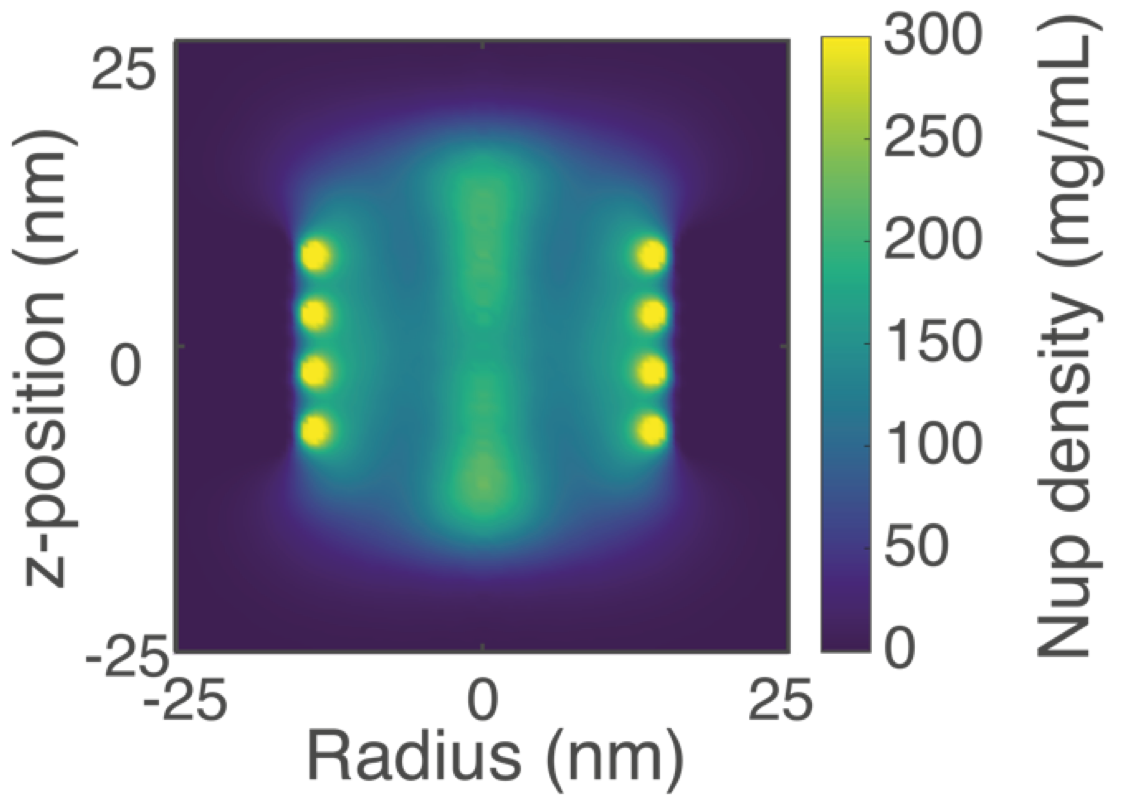
\includegraphics[width=0.6\linewidth]{figures/Figure4.24.png}
	\caption{Axi-radial density map of the protein density distribution in a 30 nm NupX-lined nanopore that interacts with Kap95 particles. The density distribution shifts towards the interface between the pore and access regions, rather than focus centrally in the pore, which is the case when no Kap95 particles are present (as shown in Figure \ref{fig:fig.4.4.1}b). }
	\label{fig:fig.4.26}	
\end{figure}
\subsection{Density distributions of NupX variations in nanopores}
\begin{figure}[H]
	\centering
	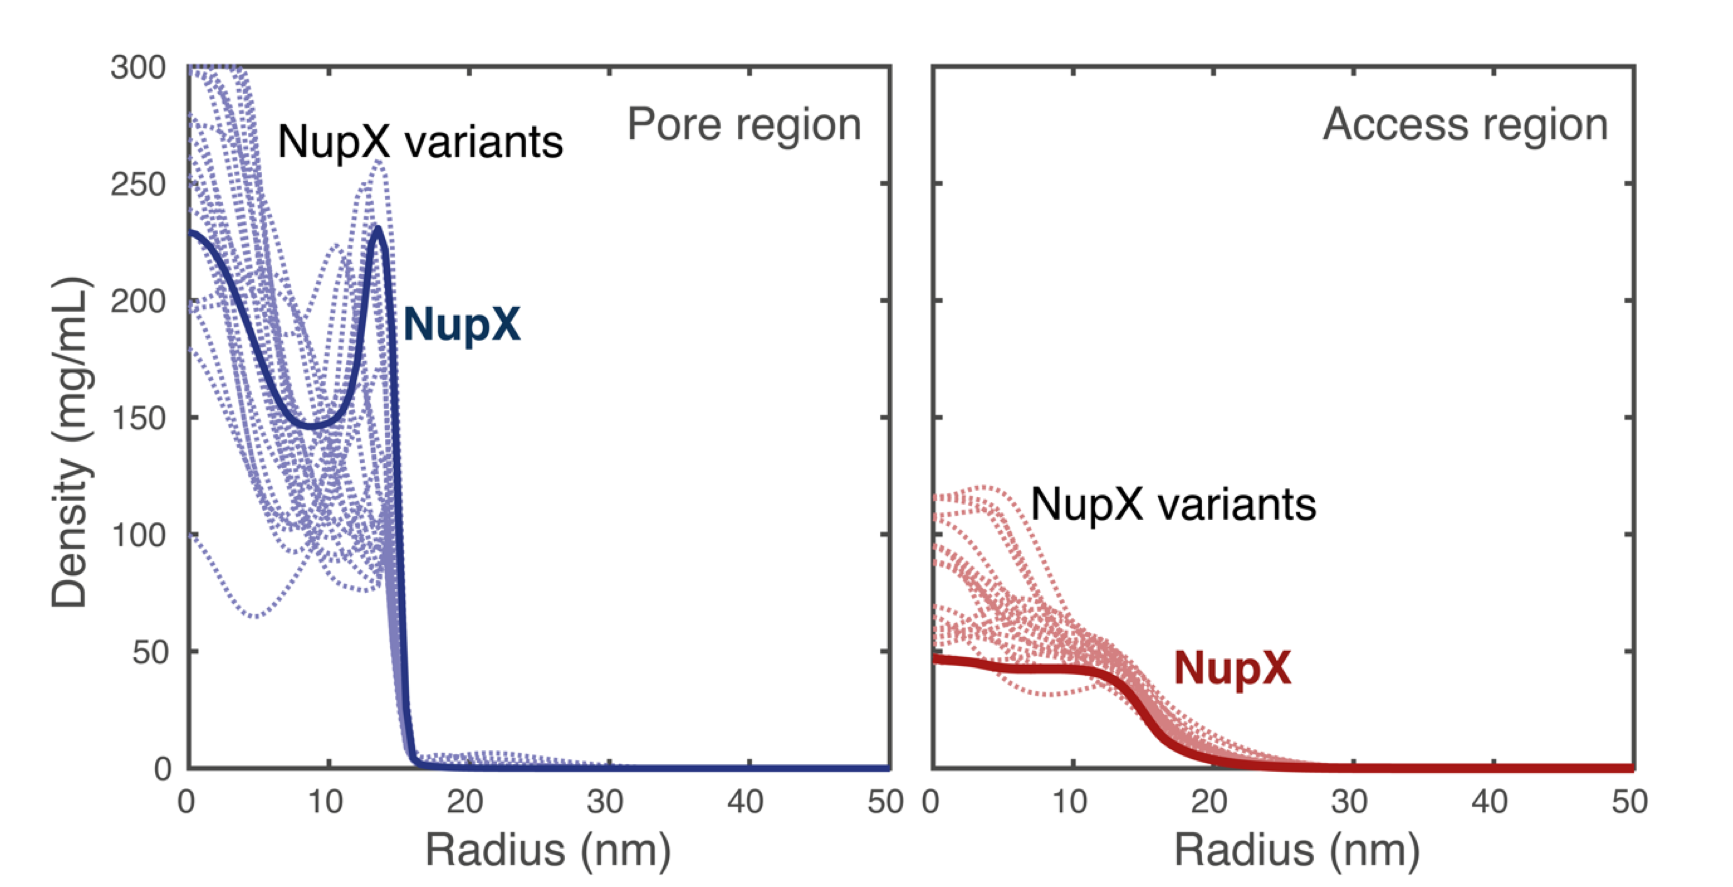
\includegraphics[width=1\linewidth]{figures/Figure4.25.png}
	\caption{Density distributions in the pore (blue dotted lines, left) and access (red dotted lines, right) regions for 25 NupX variants from Table \ref{tab:table4.2}2. NupX (bold lines) is shown for reference.}
	\label{fig:fig.4.27}	
\end{figure}
\renewcommand{\thefigure}{\thechapter.\arabic{figure}}
\renewcommand{\thetable}{\thechapter.\arabic{table}}
\renewcommand{\theequation}{\thechapter.\arabic{equation}}


\references{chapter-4/chapter-4}


